%%% main.tex — SF6 ICP Etch Surrogate Model Report
%%% Reframed: new work since last meeting (solver already known)
\documentclass[12pt,a4paper]{article}

% ---------- packages ----------
\usepackage[margin=1in]{geometry}
\usepackage{amsmath,amssymb}
\usepackage{booktabs}
\usepackage{graphicx}
\usepackage[colorlinks=true,linkcolor=blue,citecolor=blue,urlcolor=blue]{hyperref}
\usepackage{siunitx}
\usepackage[round]{natbib}
\usepackage{float}
\usepackage{caption}
\usepackage{subcaption}

\graphicspath{{../figures/}}
\tolerance=1000
\emergencystretch=1em

\sisetup{
  separate-uncertainty = true,
  multi-part-units     = single,
}

\title{%
  From Fluid Solver to Production Surrogate:\\
  PINN Failure, Supervised Learning Success,
  and LXCat Cross-Section Insights\\
  for SF\textsubscript{6}/Ar ICP Etch Modelling}

\author{%
  M.\ Abdelghany$^{*}$ \and Z.\ Ngan \\
  \textit{$^{*}$muabdelghany@gmail.com,\quad ngankait@gmail.com}}

\date{5 May 2026}

% ------------------------------------------------------------------
\begin{document}
\maketitle

% ==================================================================
\begin{abstract}
Starting from the validated 2D axisymmetric fluid solver for a TEL
SF\textsubscript{6}/Ar inductively coupled plasma (ICP) etcher, we
report three lines of investigation pursued since the last meeting.
First, a physics-informed neural network (PINN) approach was attempted
and failed: PDE-constrained training diverges due to five interacting
root causes, while data-only training converges readily
($23{,}000\times$ loss reduction), motivating a pivot to supervised
surrogates.  Second, a systematic surrogate development progressed
through four generations---v1 (nF RMSE 0.133), v2 (0.111), v3
(0.023), v4 (0.003)---via data enrichment, physics regularisation, and
ensemble uncertainty quantification, achieving a $524\times$ speedup
over the legacy solver.  Third, integration of LXCat/Biagi
cross-section data revealed that the electron temperature increases by
56\% and electron density decreases by 69\%, while F density is
unchanged.  A controlled architecture sweep (7 experiments, 3 seeds
each) identified the E3\_separate\_heads topology as the winner.  The
recipe was then applied per species to build a complete multi-species
surrogate covering all 21 outputs of the 2D solver (9 neutrals: SF$_n$
for $n\!\in\![1,6]$, F, F$_2$, S; 11 charged: $n_e$, $n_{+}$, $n_{-}$,
F$^{+}$/F$^{-}$, SF$_3^{+}$, SF$_4^{\pm}$, SF$_5^{\pm}$, SF$_6^{-}$;
and electron temperature $T_e$).  Each species is fit by an independent
5-model single-head ensemble; RMSEs span 0.00145 (nSF$_6$) to 0.01019
($n_e$) on $\log_{10}$ density.  The full 21-species ensemble evaluates
one operating point in $\sim$\SI{283}{\milli\second}, a
$27\times$/$51\times$ speedup over the legacy/LXCat solvers respectively.
Ablation (on the lead species) reveals output-bias initialisation as
the dominant factor (74\% of RMSE reduction on nF).  Limitations are
discussed candidly, including a 36\% systematic error in absolute F
density versus published measurements.
\end{abstract}

\newpage
\tableofcontents
\newpage

% ==================================================================
\section{Introduction}
\label{sec:intro}

In our last meeting we reviewed the two-dimensional axisymmetric fluid
solver for a TEL inductively coupled plasma (ICP) etcher operating in
SF\textsubscript{6}/Ar mixtures.  That solver---with its 54-reaction
Arrhenius chemistry set~\citep{lallement2009}, drift--diffusion
transport, and Robin boundary conditions---is now the established
baseline.  This report covers everything accomplished since then.

Three directions were pursued:
\begin{enumerate}
  \item \textbf{PINN for spatial acceleration
        (Section~\ref{sec:pinn}):} We attempted to embed the governing
        PDEs directly into the neural-network loss function.  This
        failed due to stiff chemistry, cylindrical singularities, and
        multi-scale loss competition.  The negative result is
        documented with a five-point root-cause analysis.
  \item \textbf{Supervised surrogate development
        (Sections~\ref{sec:surrogate}--\ref{sec:production}):}
        Pivoting from PINNs, we built a feedforward surrogate that
        progressed through four generations (v1--v4) and then underwent
        a controlled architecture sweep, ablation study, and ensemble
        optimisation to reach production quality.
  \item \textbf{LXCat physics upgrade
        (Section~\ref{sec:lxcat}):} Biagi cross sections were
        integrated into the solver.  The physics impact was dramatic
        ($T_e$ +56\%, $n_e$ $-$69\%, F unchanged), but a dataset
        diagnosis revealed that the 3.85$\times$ RMSE gap between
        legacy and LXCat surrogates was caused by the training recipe,
        not physics difficulty.
\end{enumerate}

The report is structured to follow this narrative arc:
Sections~\ref{sec:recap}--\ref{sec:sim_recap} briefly recap the
solver (already reviewed); Section~\ref{sec:pinn} documents the PINN
failure; Sections~\ref{sec:surrogate}--\ref{sec:production} present
the surrogate development; Section~\ref{sec:lxcat} covers the LXCat
integration; Sections~\ref{sec:arch_sweep}--\ref{sec:ablation}
describe the architecture search and ablation;
Section~\ref{sec:validation} presents validation;
Section~\ref{sec:supplementary} reports supplementary experiments; and
Sections~\ref{sec:discussion}--\ref{sec:conclusion} discuss findings
and conclude.

% ==================================================================
\section{Solver Recap}
\label{sec:recap}

This section provides a brief summary of the 2D TEL fluid solver for
readers' convenience; full details were presented at the last meeting.

\subsection{Geometry and Governing Equations}

The reactor is a TEL ICP etcher with a T-shaped axisymmetric geometry
comprising an ICP source ($R = \SI{38}{\milli\metre}$,
$L = \SI{181.5}{\milli\metre}$), a \SI{2}{\milli\metre} aperture, and
a processing chamber ($R = \SI{105}{\milli\metre}$,
$L = \SI{50}{\milli\metre}$) where the wafer sits
(Figure~\ref{fig:geom_pair}).  The solver discretises continuity
equations for each species on a structured $(r, z)$ mesh with
drift--diffusion transport, Robin boundary conditions at material
walls~\citep{kokkoris2008}, and the 54-reaction Arrhenius chemistry
set of \citet{lallement2009}.  An electron energy equation provides
$T_e$.

\begin{figure}[H]
  \centering
  \begin{subfigure}[t]{0.48\textwidth}
    \centering
    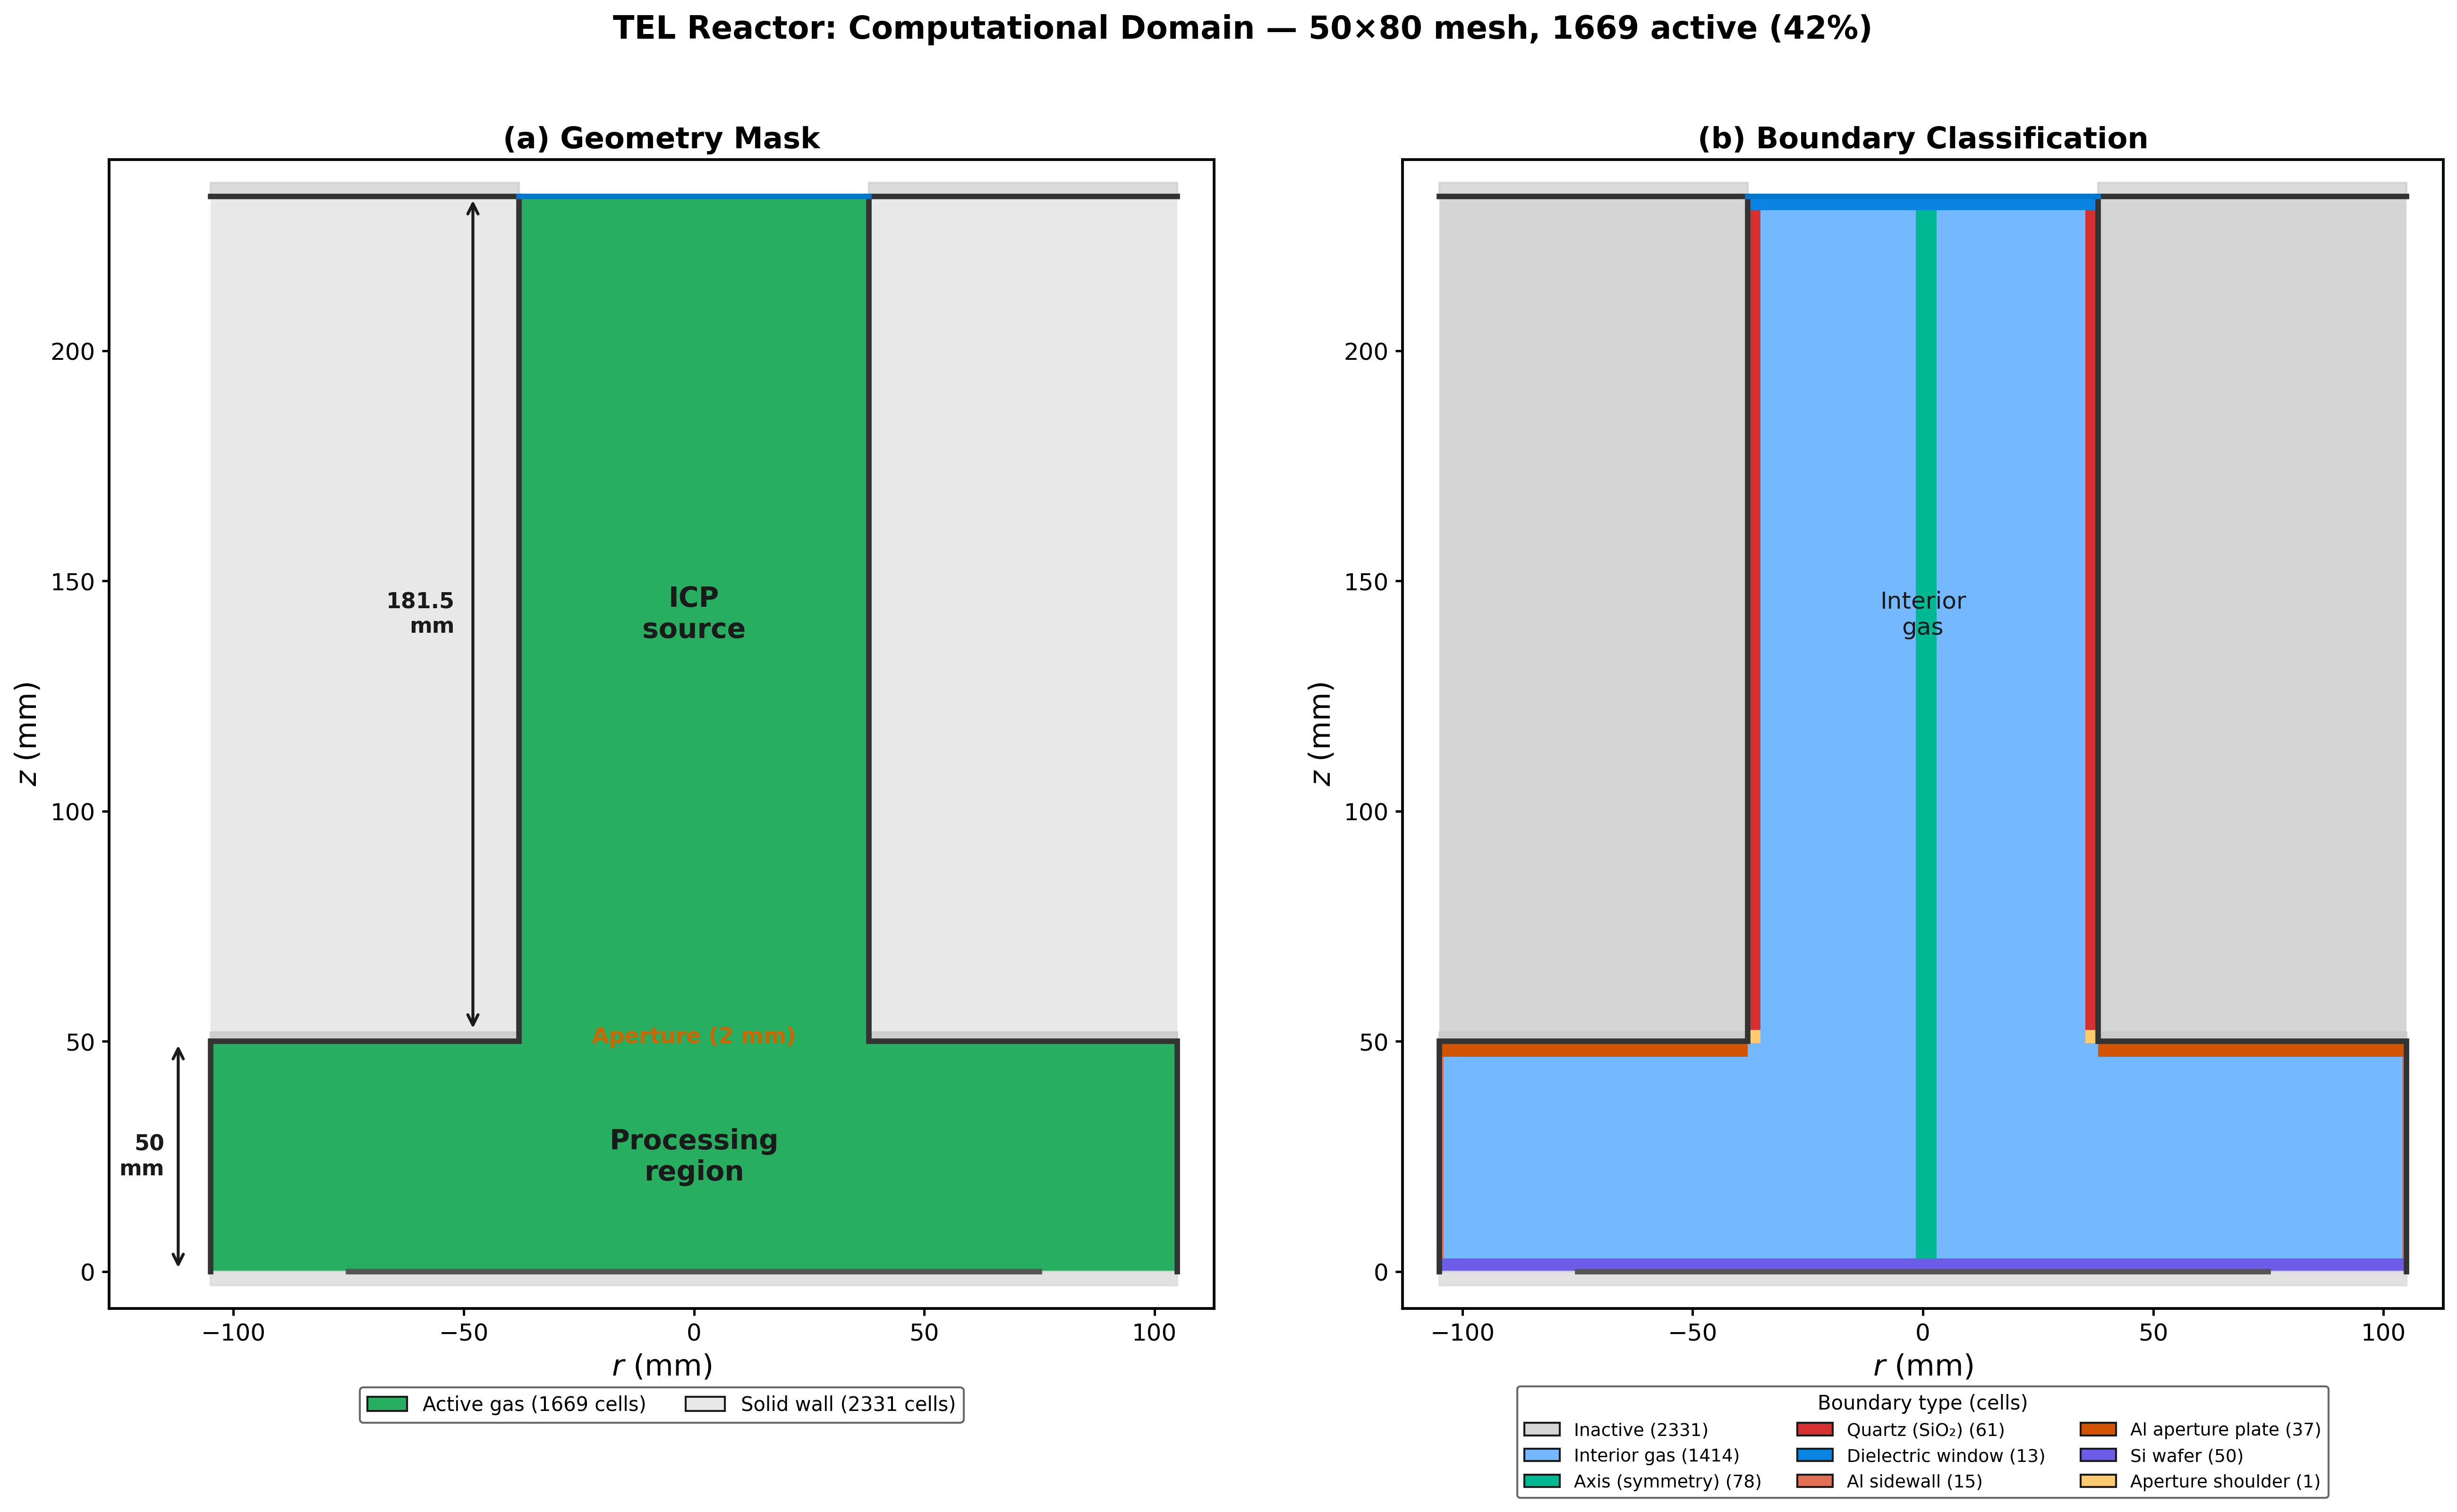
\includegraphics[width=\textwidth]{geometry_mask.png}
    \caption{Full reactor geometry showing the ICP source,
             aperture, and processing regions with the
             computational mask.}
    \label{fig:geometry}
  \end{subfigure}
  \hfill
  \begin{subfigure}[t]{0.48\textwidth}
    \centering
    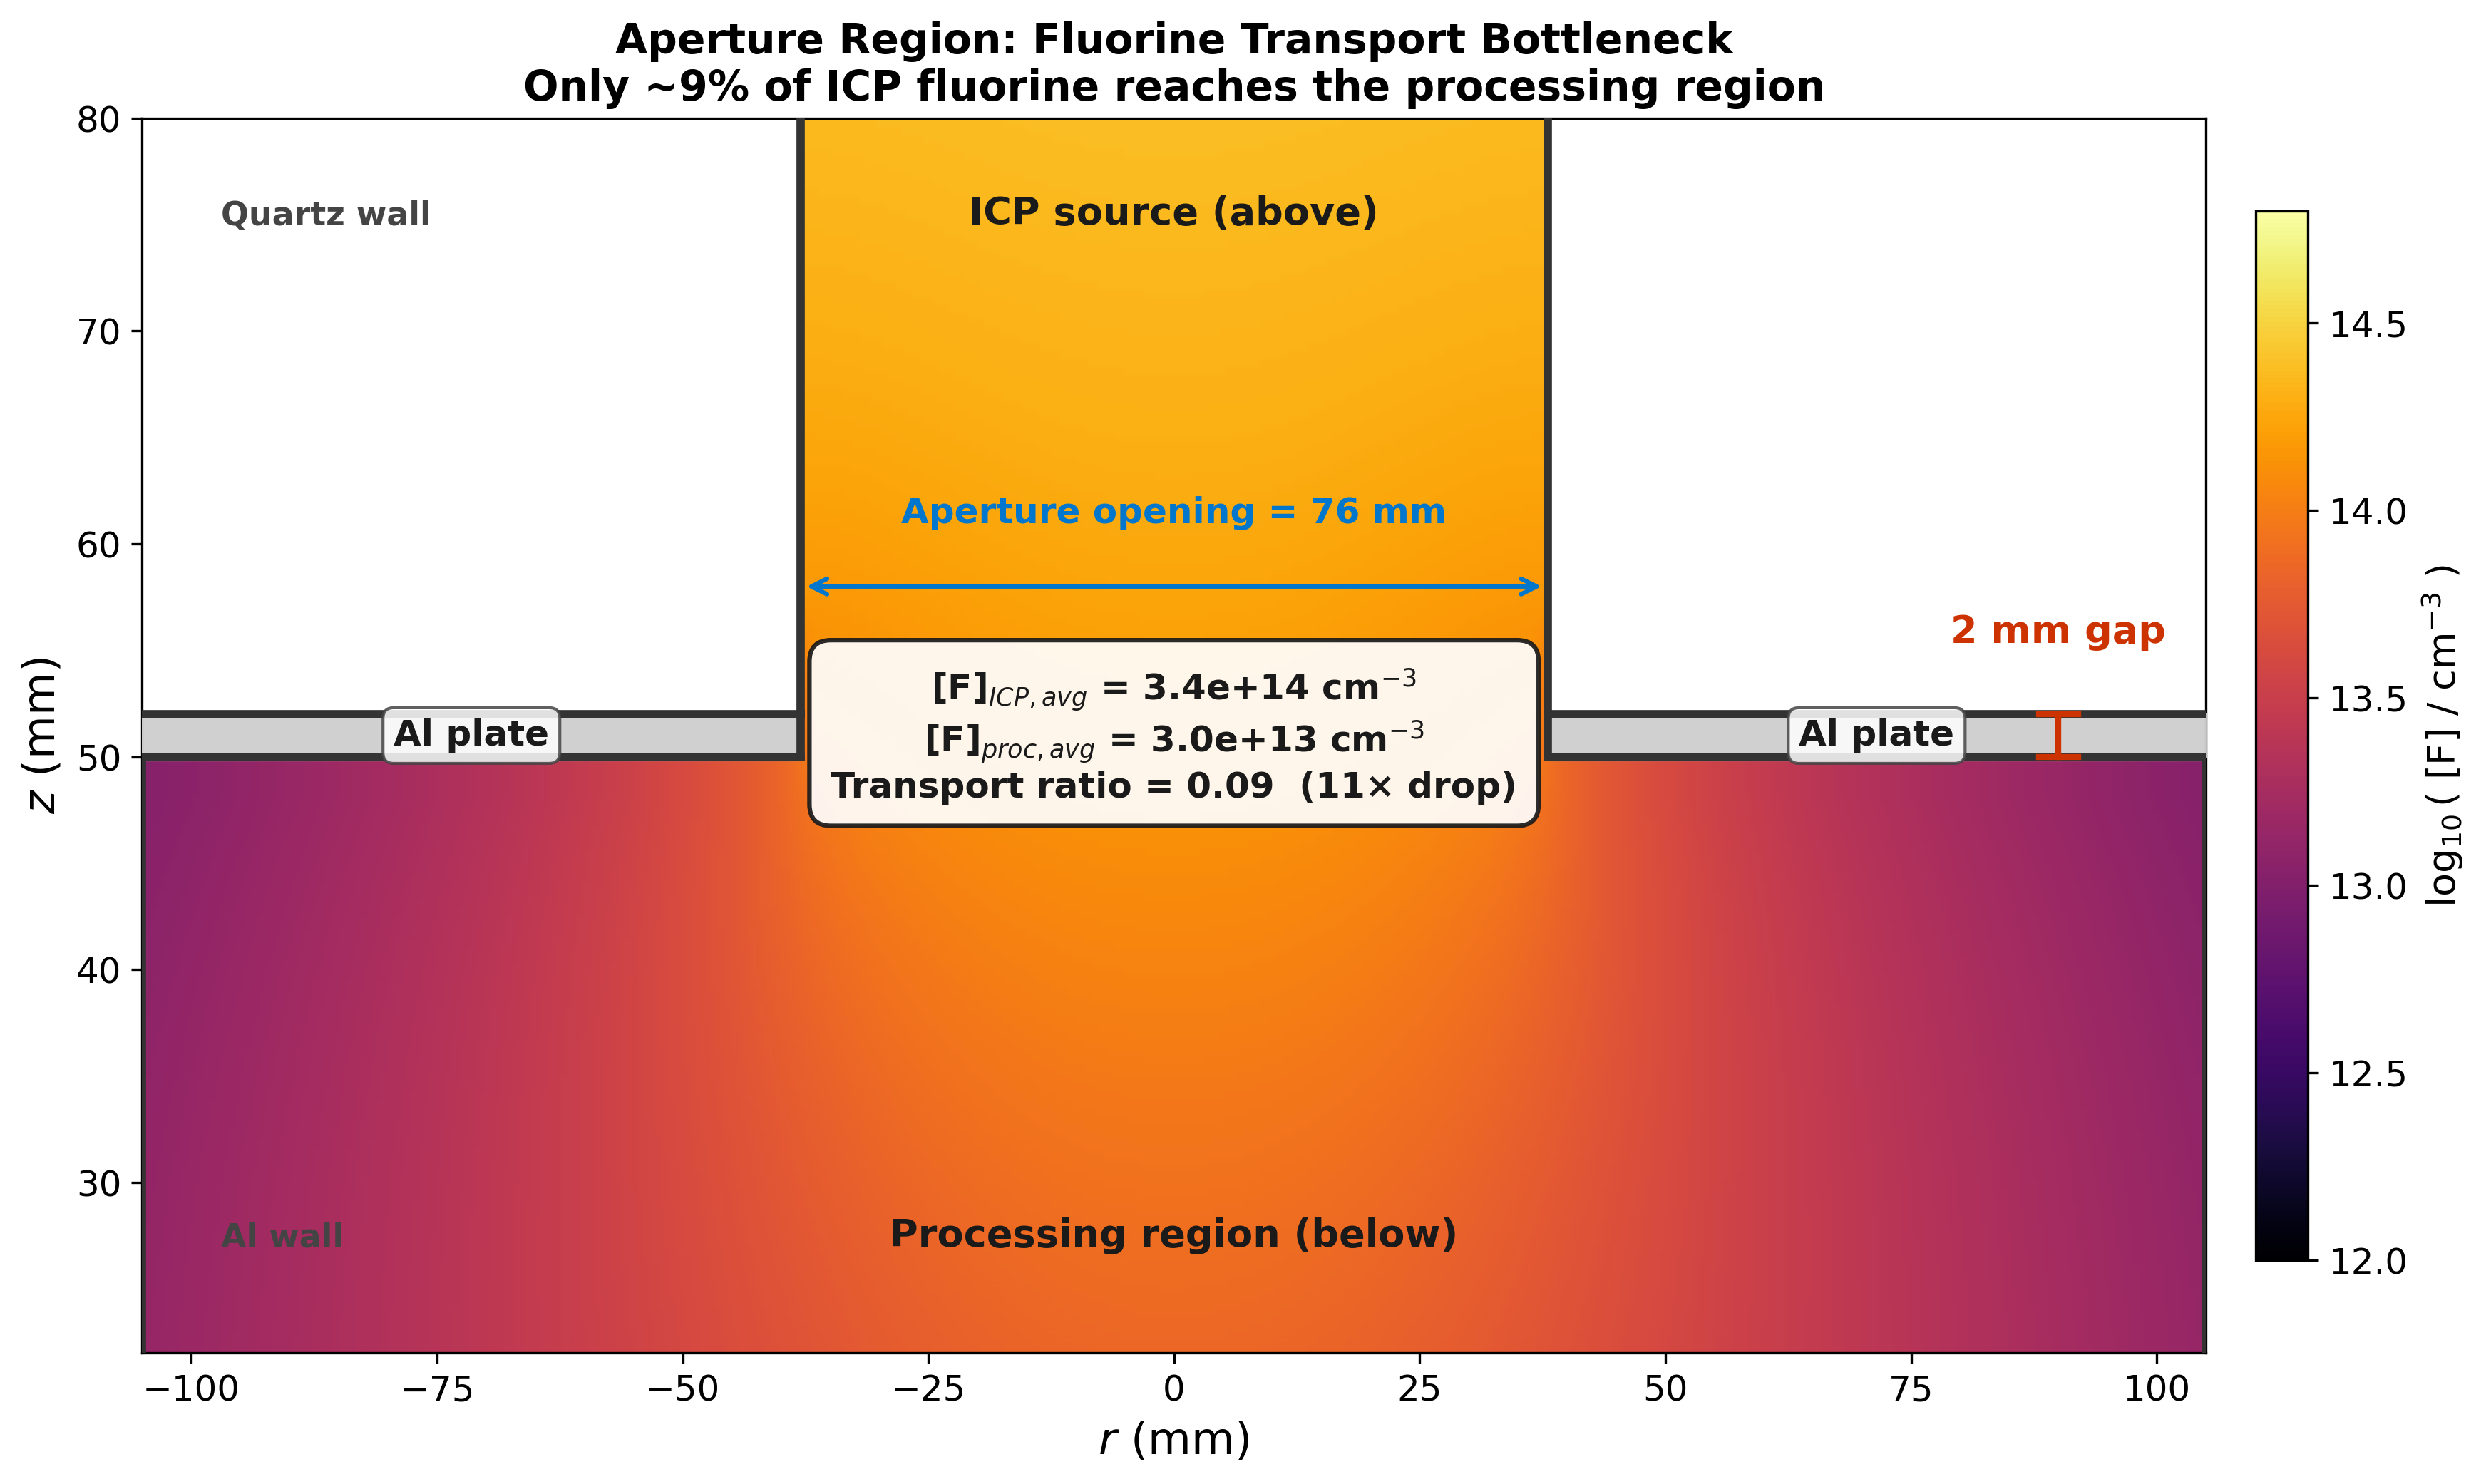
\includegraphics[width=\textwidth]{aperture_zoom.png}
    \caption{Zoomed view of the aperture region connecting the
             ICP source to the processing chamber.}
    \label{fig:aperture}
  \end{subfigure}
  \caption{Reactor geometry.  The T-shaped domain is solved in 2D
           axisymmetric cylindrical coordinates.}
  \label{fig:geom_pair}
\end{figure}

\subsection{Solver Performance and Operating Ranges}

The legacy solver (tabulated cross sections) requires
\SI{7.76}{\second} per operating-point evaluation; the LXCat solver
increases this to \SI{14.4}{\second}.  The operating-parameter space
spans $P_{\text{rf}} \in [200, 1200]\;\si{\watt}$,
$p \in [3, 20]$~mTorr, and $x_{\text{Ar}} \in [0, 50]\%$.
Figure~\ref{fig:em_power} shows the electromagnetic power deposition
profile that drives the discharge.

\begin{figure}[H]
  \centering
  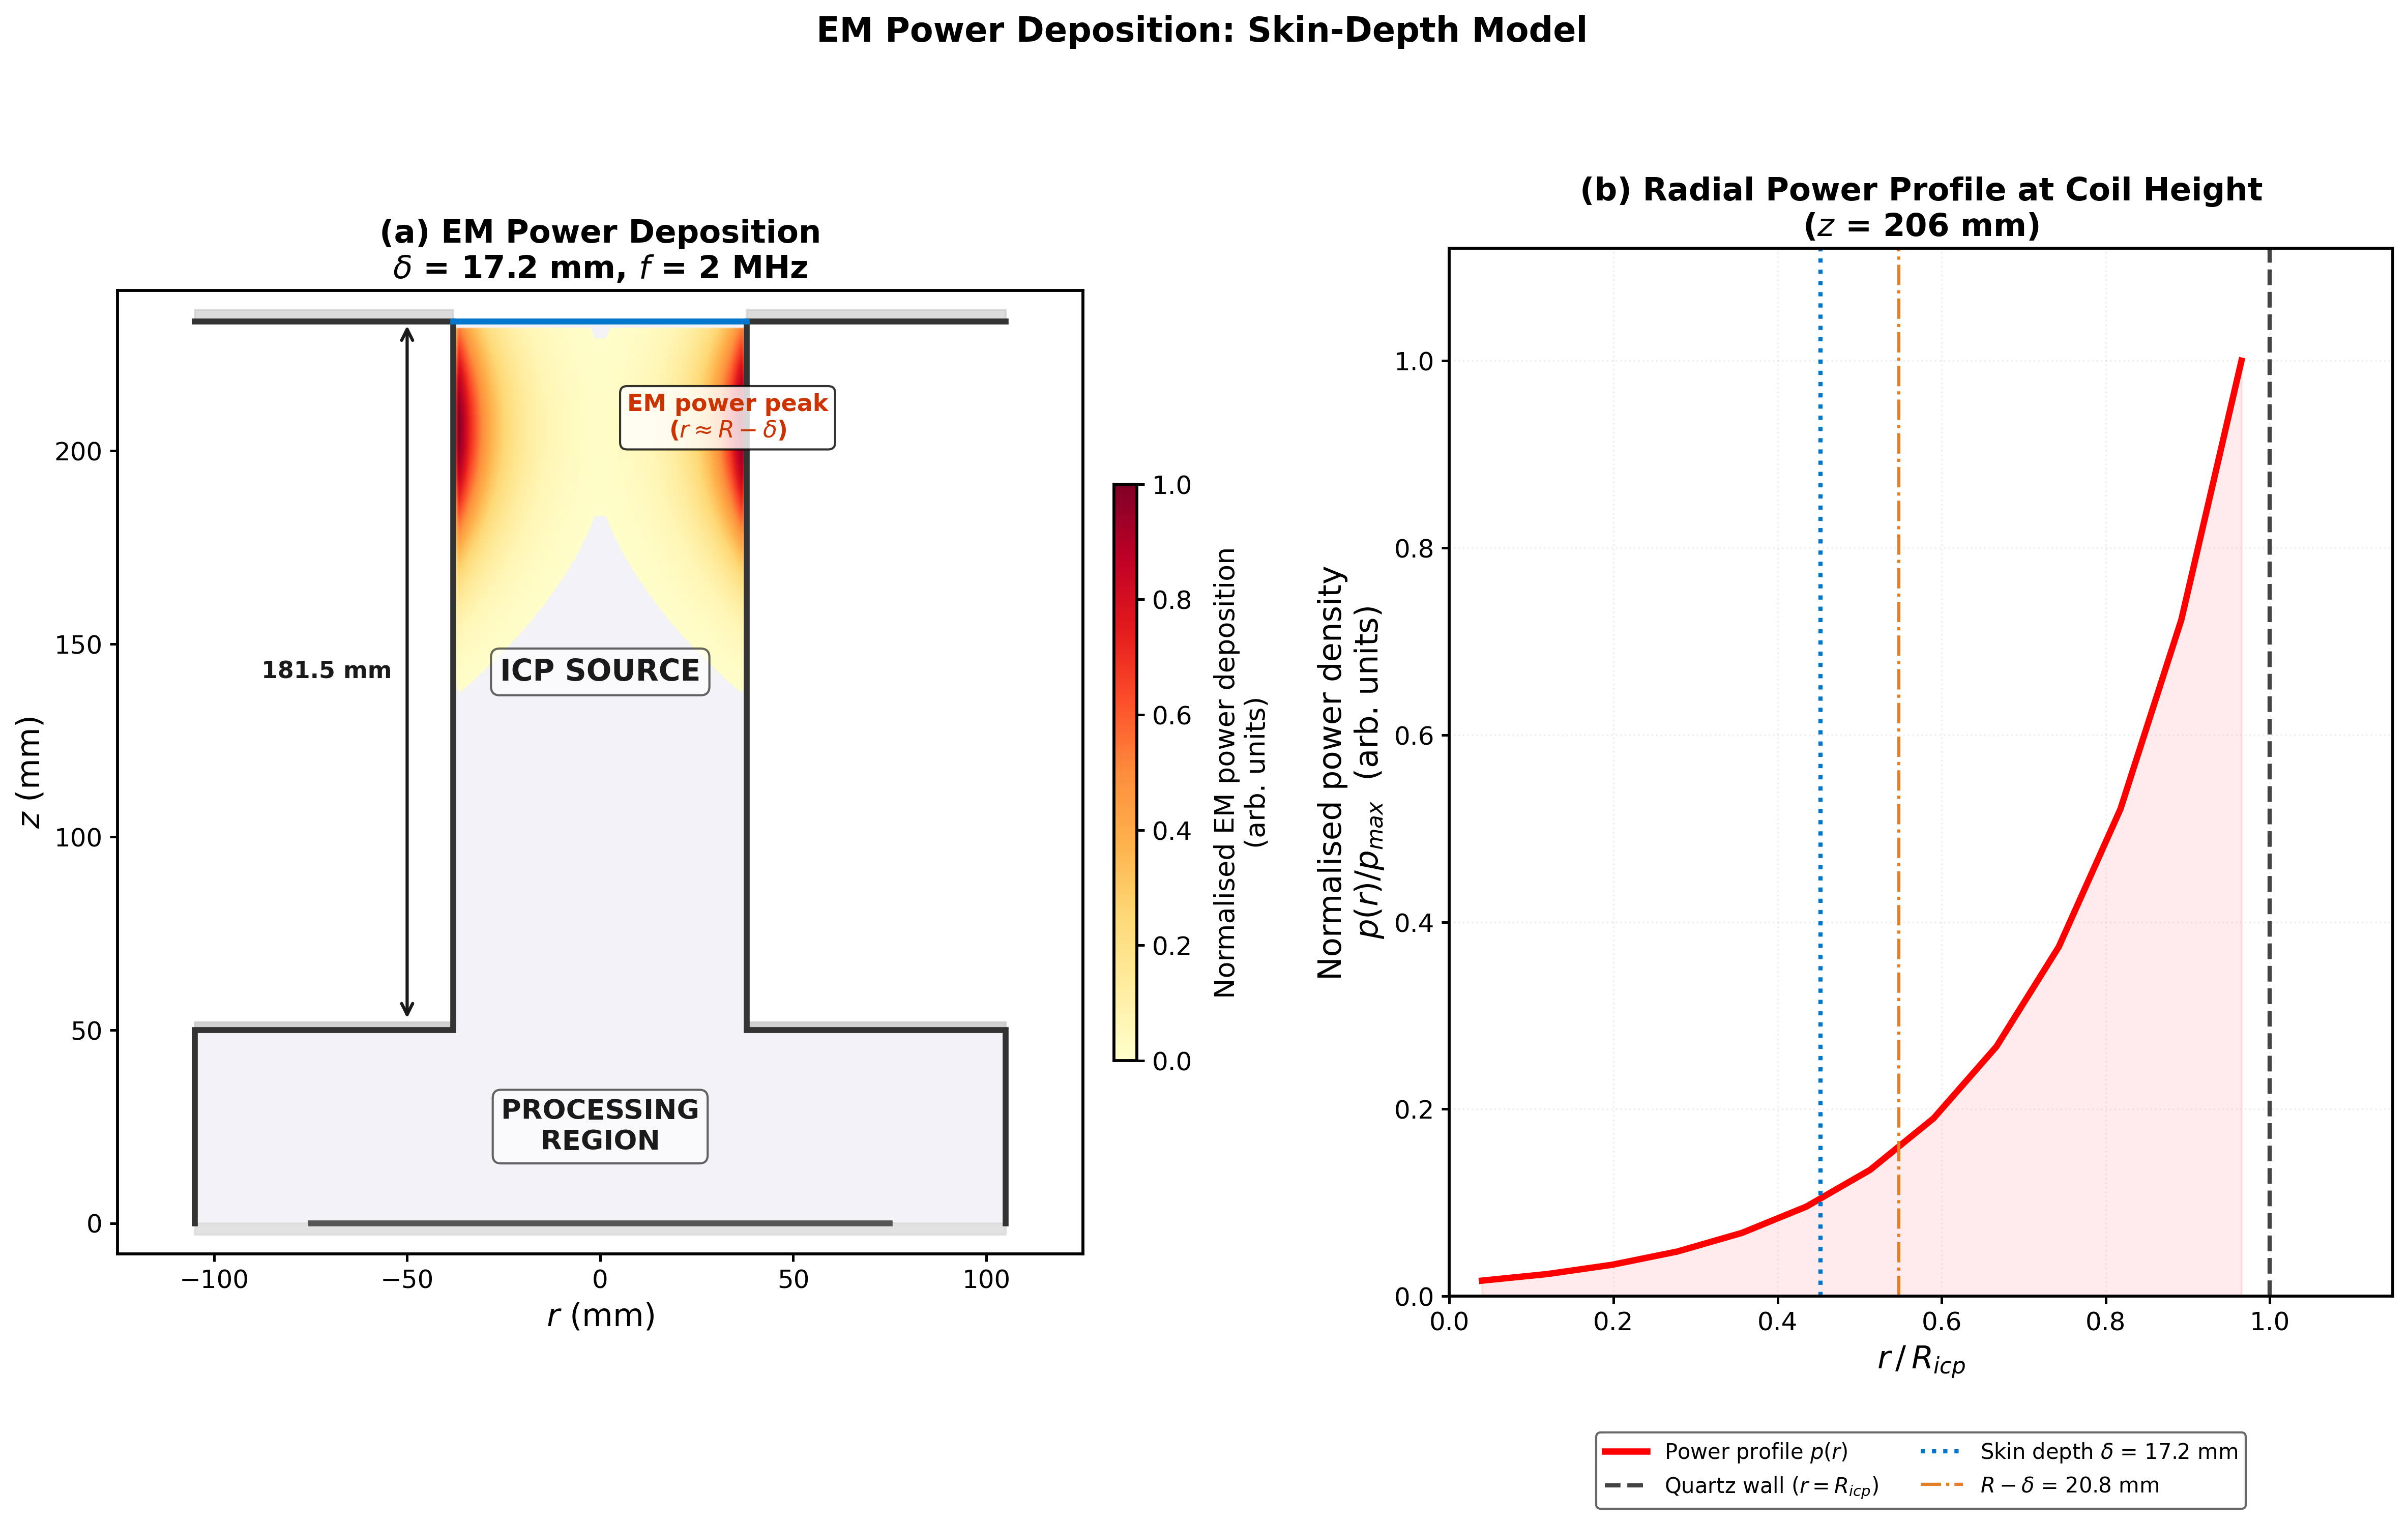
\includegraphics[width=0.55\textwidth]{em_power_deposition.png}
  \caption{Electromagnetic power deposition profile in the ICP
           source region.  Power is concentrated near the coil
           windings and decays exponentially with the skin depth.}
  \label{fig:em_power}
\end{figure}

\paragraph{Phase-1 6b refitting since main.pdf v1.}
The solver underlying the LXCat dataset in this report differs from
main.pdf v1 in two material ways.  First, the bottom-boundary BC map
in \texttt{build\_geometry\_mask} was corrected to split the
\(j=0\) row into \texttt{BC\_WAFER} (\(r \le 0.075\,\mathrm{m}\),
silicon) and \texttt{BC\_AL\_TOP} (\(r > 0.075\,\mathrm{m}\),
aluminium pedestal-top / chamber-floor annulus).  Prior code labelled
the entire bottom as \texttt{BC\_WAFER}, undercounting the Al
F-sink by an annulus of area \(\sim 0.017\,\mathrm{m}^2\) (about
96\,\% of the wafer area).  Second, a hold-out refit of
\(\gamma_\mathrm{Al}\) was attempted on the corrected BC map: fitted
on the 90\,\% SF\textsubscript{6} bias-on condition, the resulting
\(\gamma_\mathrm{Al}^*\) \emph{failed} all three held-out
compositions (residuals change sign across the composition axis,
from \(-21.7\,\%\) at 90\,\% SF\textsubscript{6} to \(+30\,\%\) at
30\,\% SF\textsubscript{6}), indicating that no scalar
\(\gamma_\mathrm{Al}\) closes the Mettler residual.  Both findings
are documented in the 6b workspace and motivate the LXCat surrogate
runs reported here, where the rate-coefficient set is the only
varying knob.

% ==================================================================
\section{Representative Solver Output}
\label{sec:sim_recap}

Before turning to the new work, we show representative solver outputs
to establish the physical phenomena the surrogate must capture.
Figures~\ref{fig:contours}--\ref{fig:bars} illustrate the spatial and
compositional structure of the discharge.

\begin{figure}[H]
  \centering
  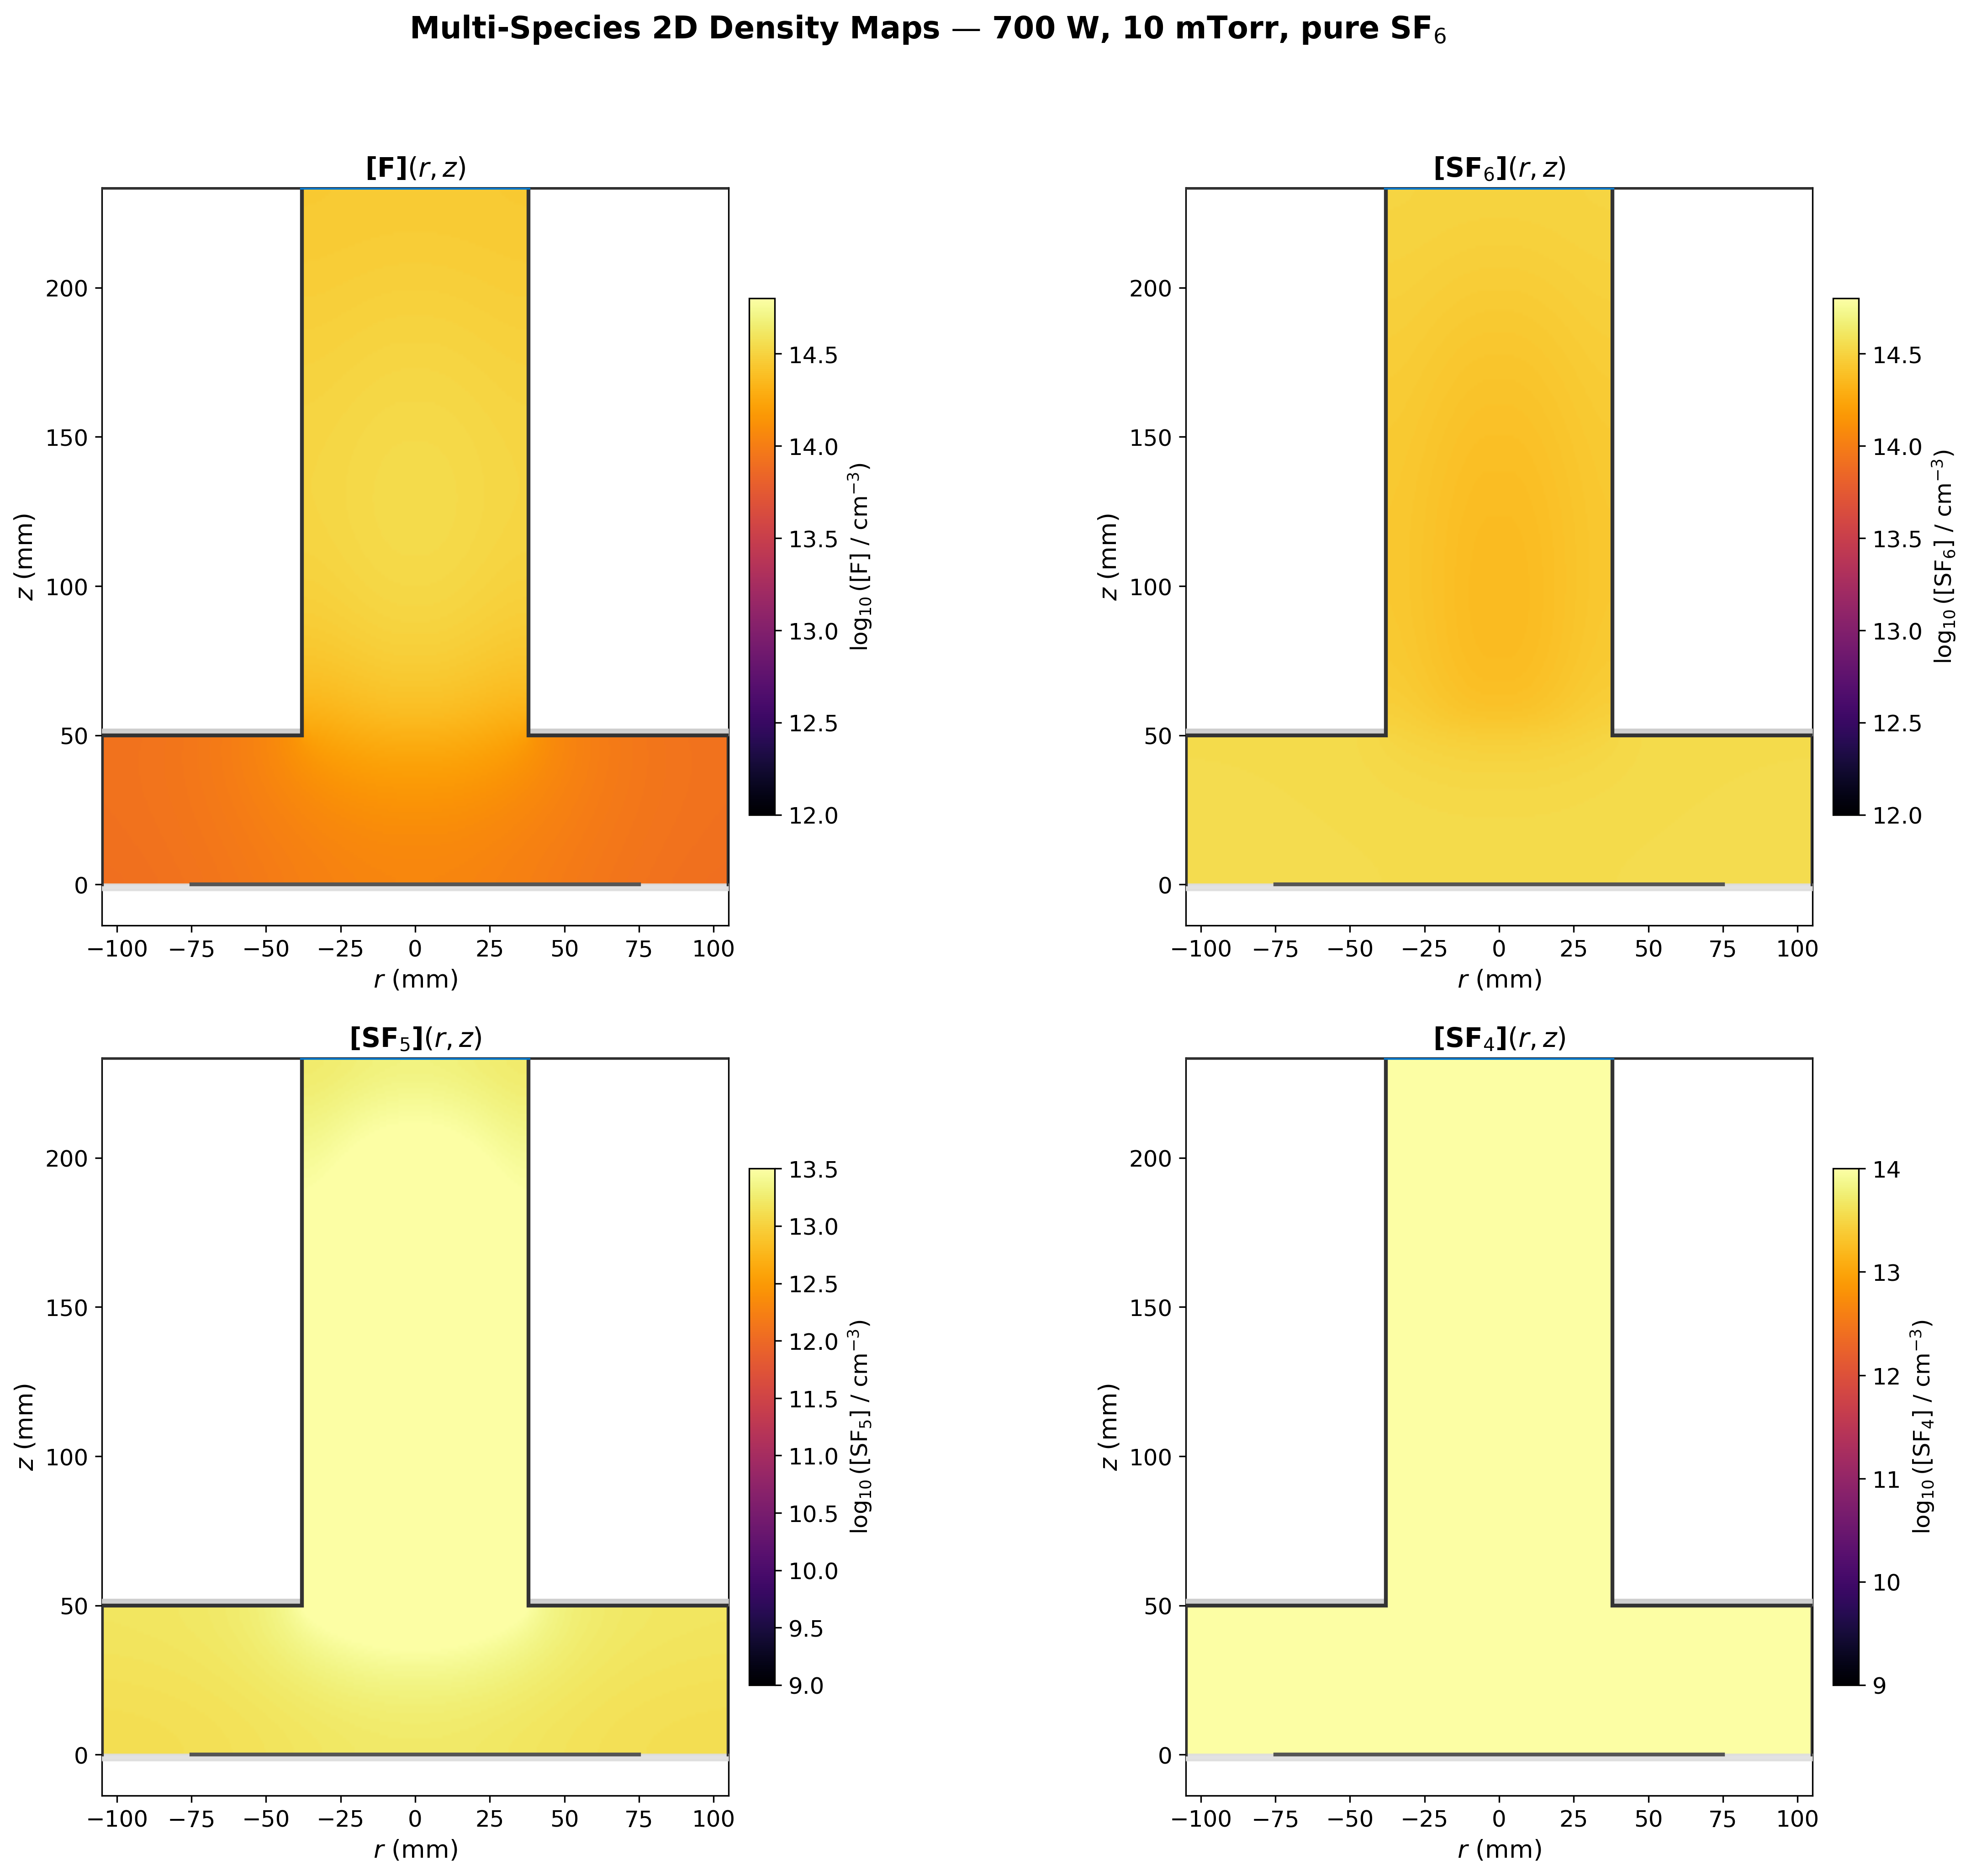
\includegraphics[width=\textwidth]{multispecies_contours.png}
  \caption{Two-dimensional density contours for major neutral and
           charged species at a representative operating point.
           Fluorine atoms are generated predominantly in the ICP
           source and diffuse through the aperture to the processing
           region.}
  \label{fig:contours}
\end{figure}

\begin{figure}[H]
  \centering
  \begin{subfigure}[t]{0.48\textwidth}
    \centering
    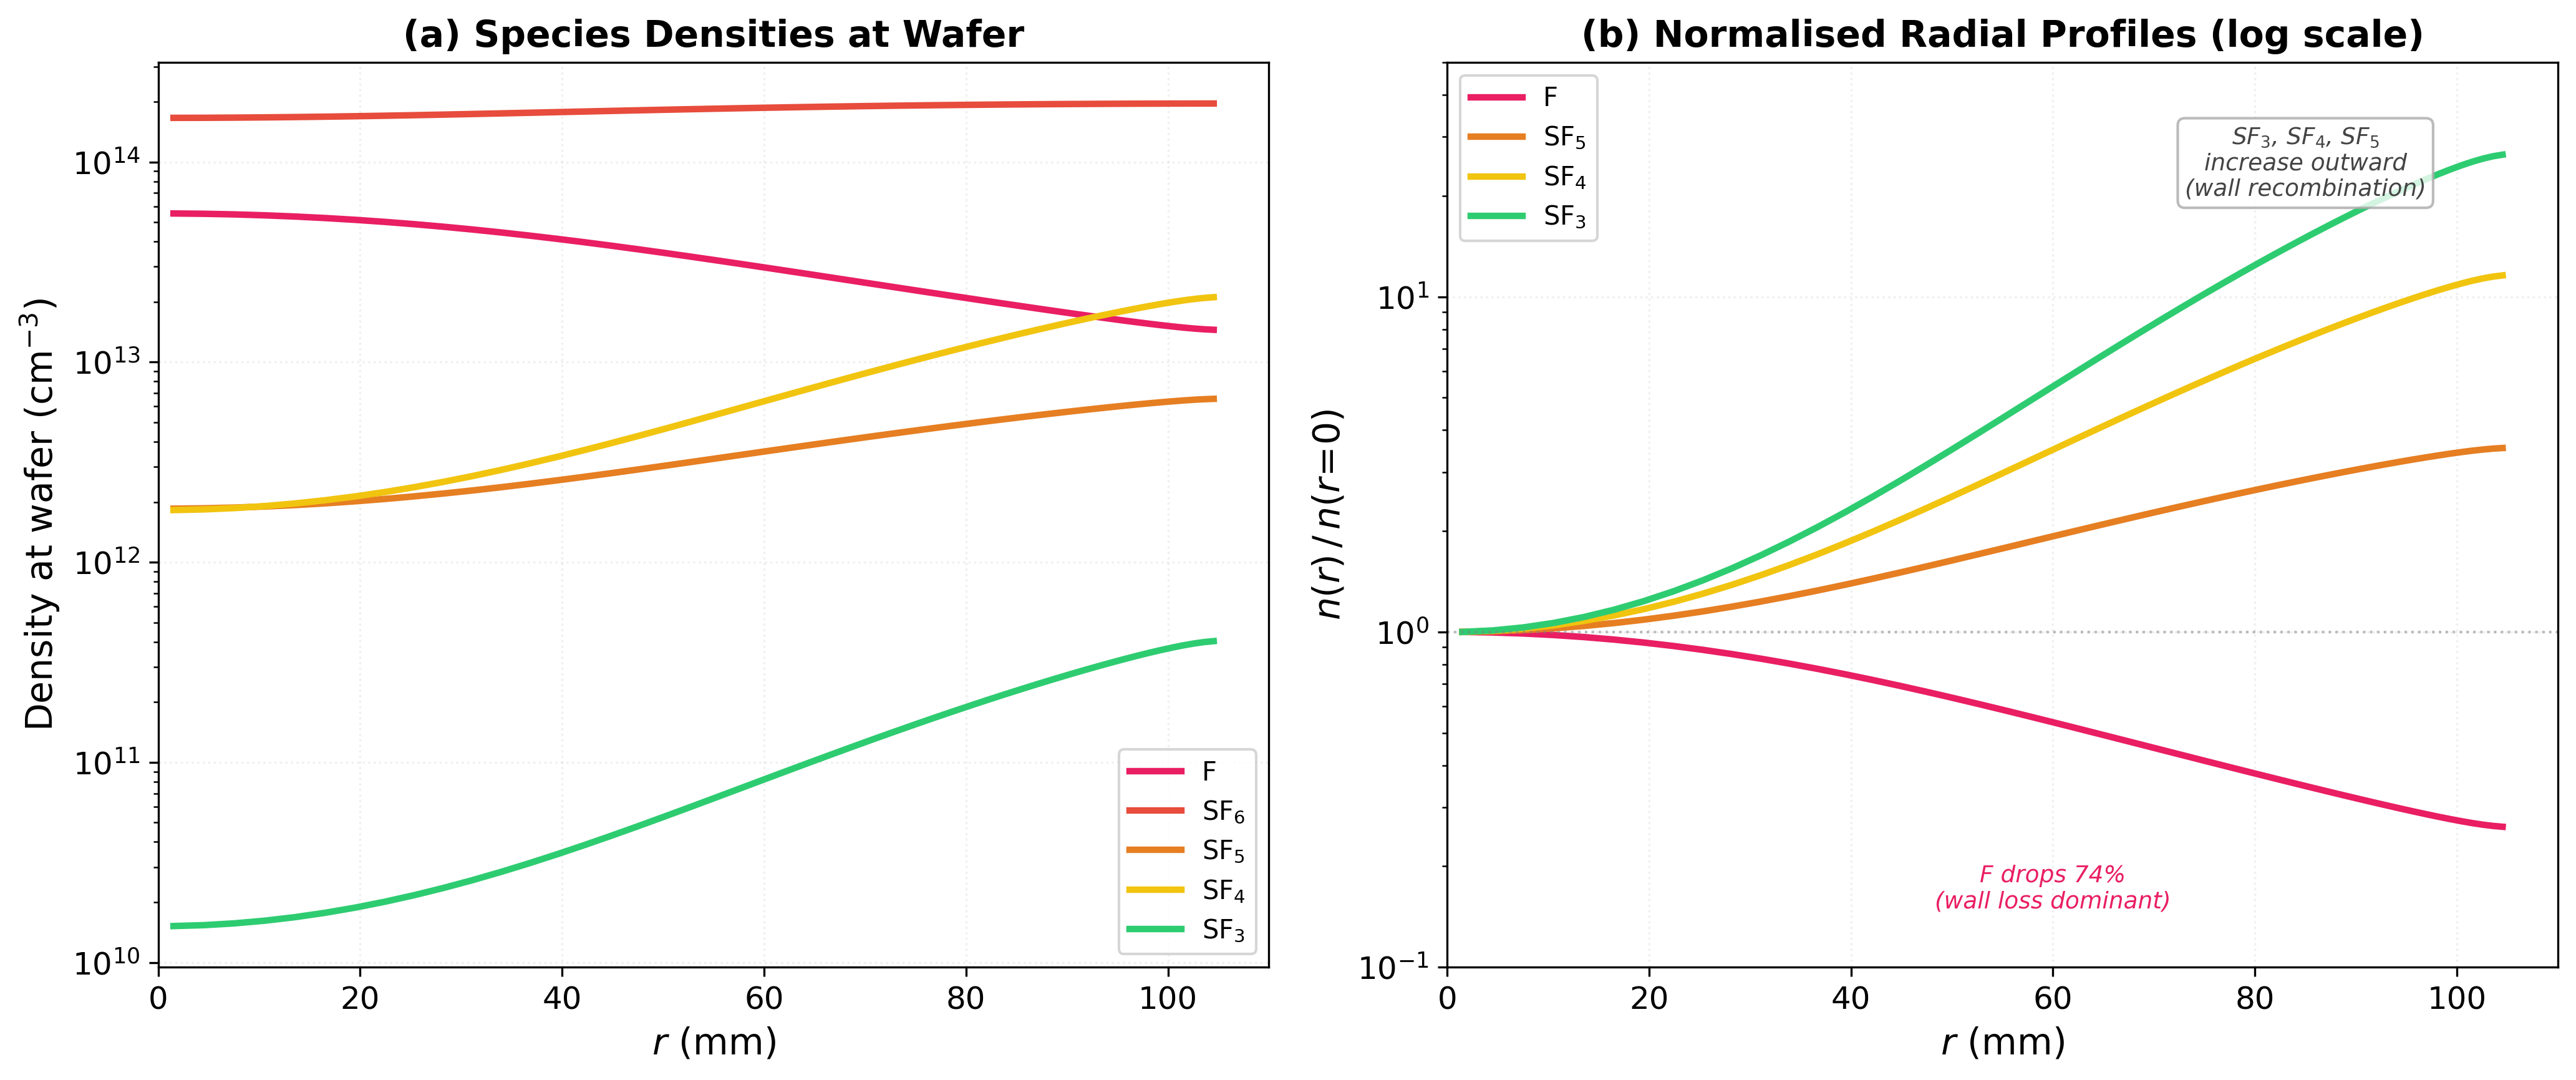
\includegraphics[width=\textwidth]{multispecies_radial.png}
    \caption{Radial profiles at the wafer surface.}
    \label{fig:radial_multi}
  \end{subfigure}
  \hfill
  \begin{subfigure}[t]{0.48\textwidth}
    \centering
    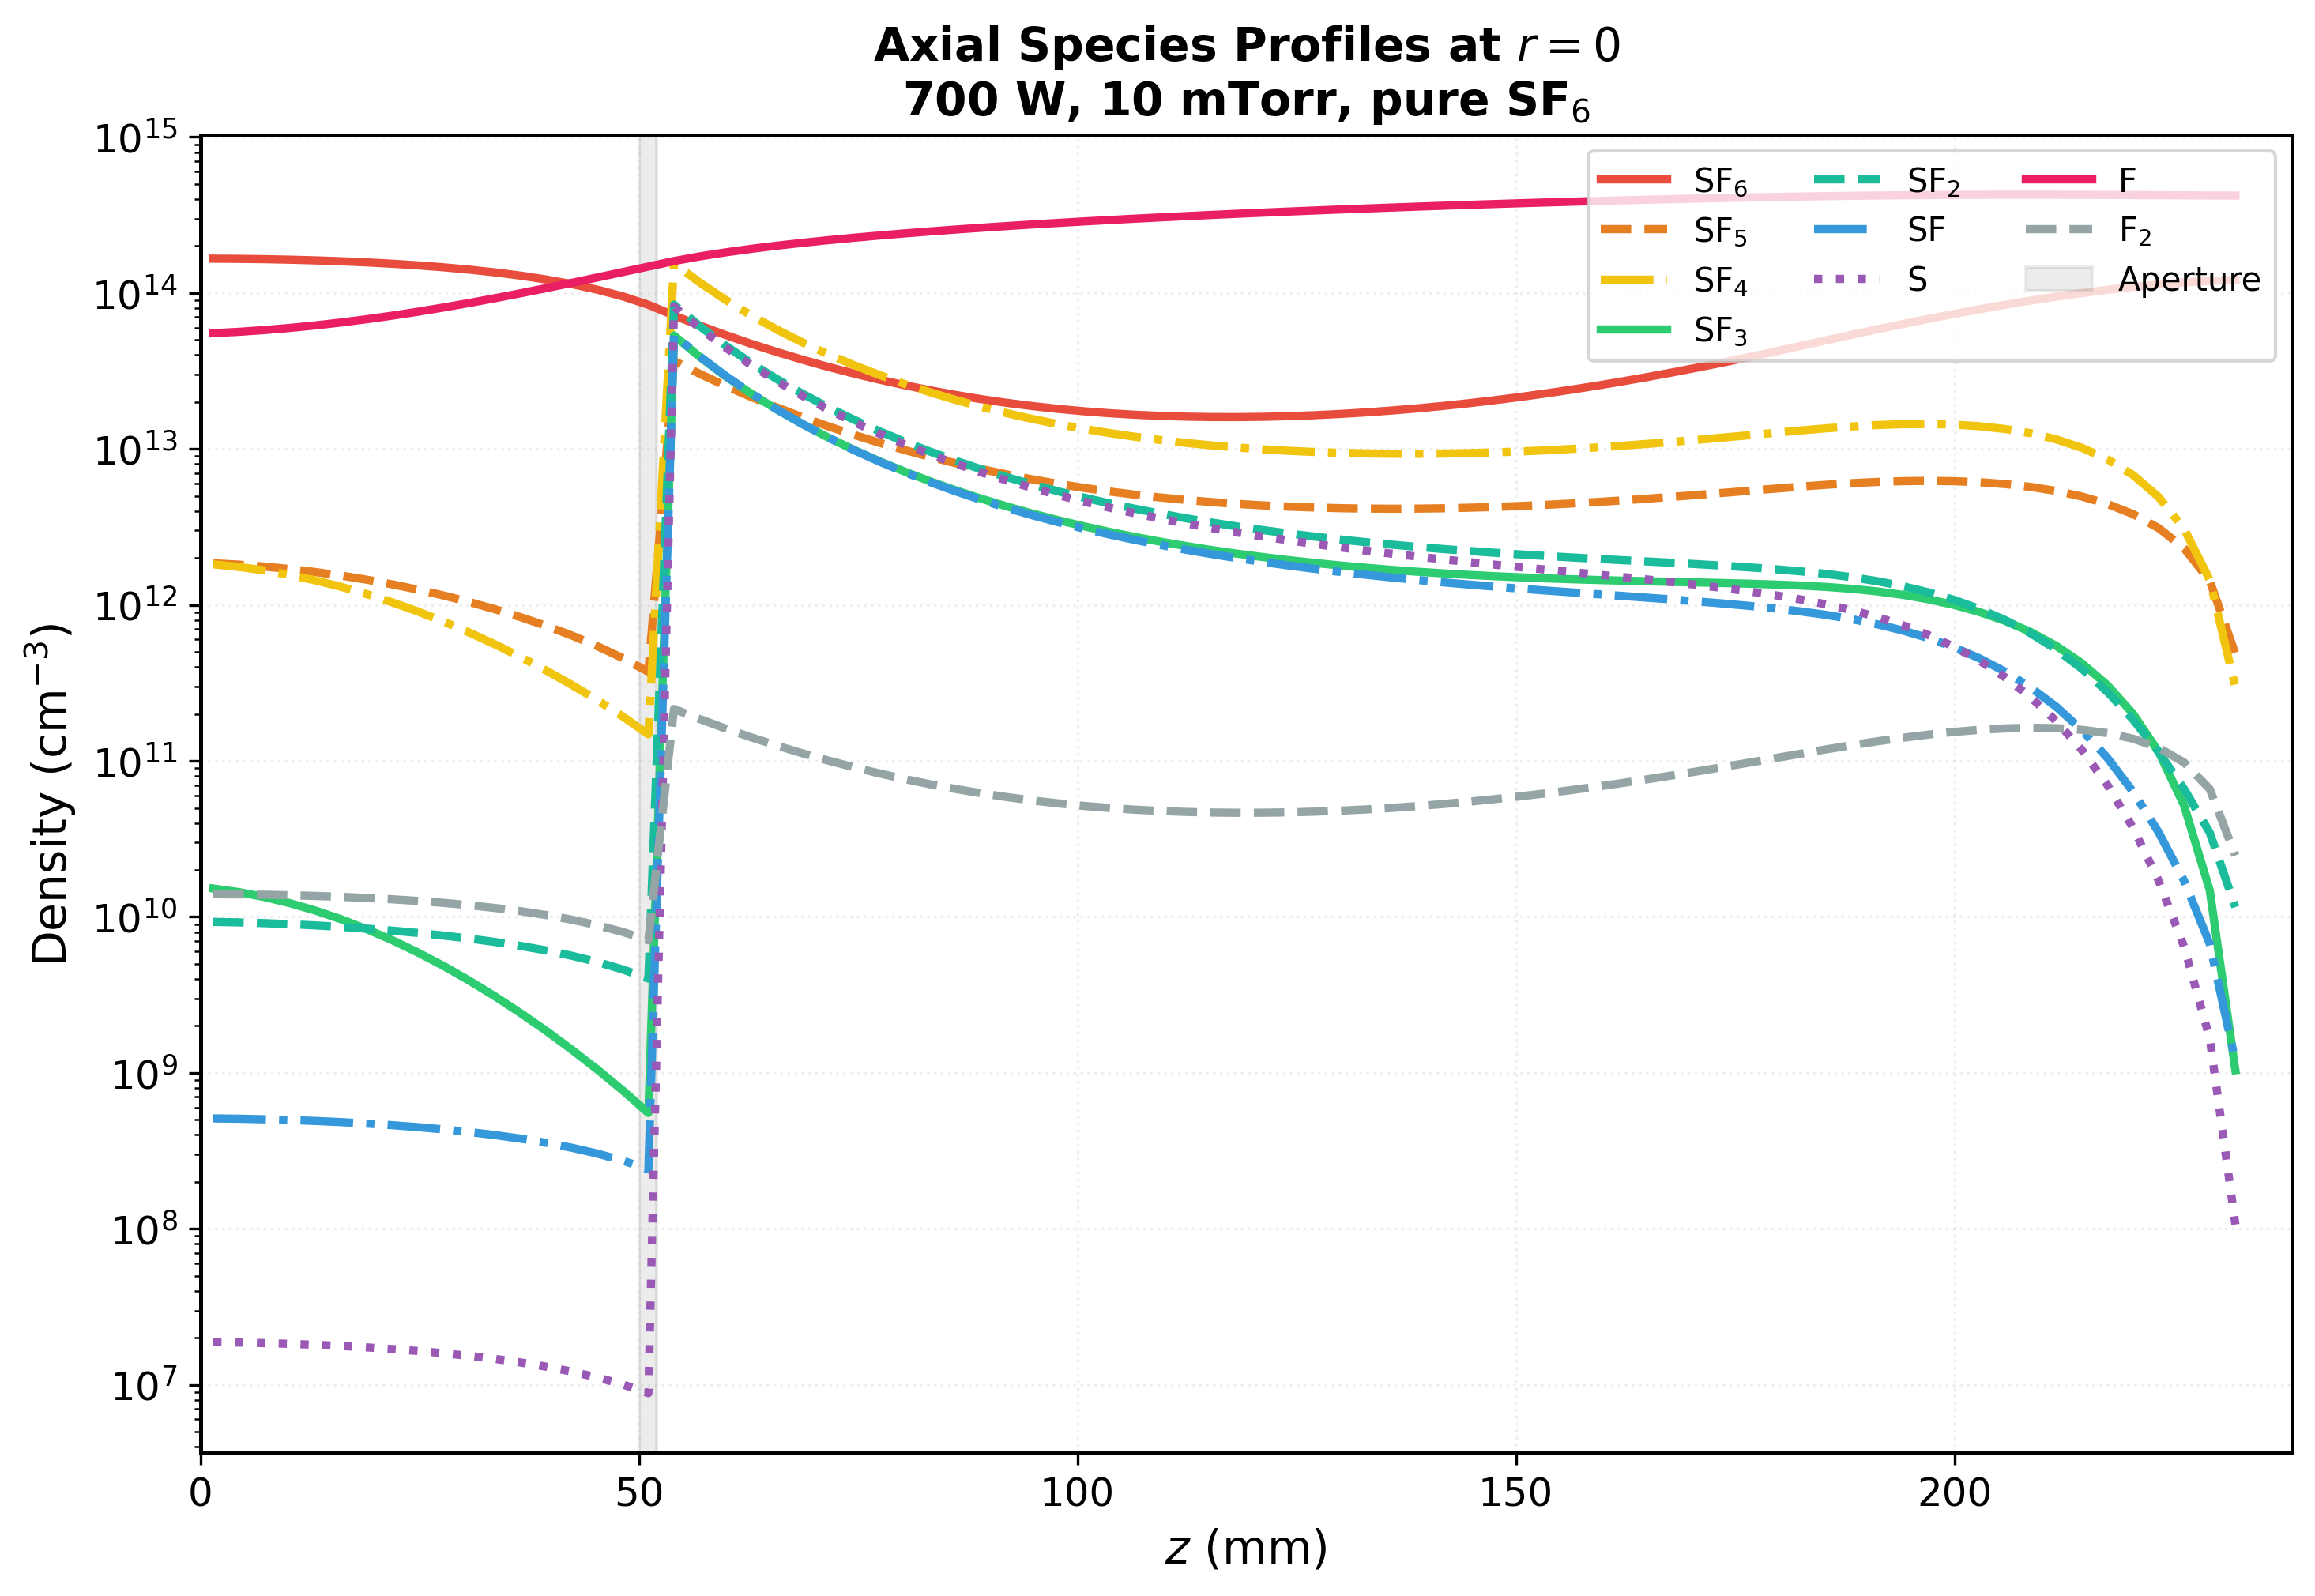
\includegraphics[width=\textwidth]{multispecies_axial.png}
    \caption{Axial profiles along the reactor centreline.}
    \label{fig:axial_multi}
  \end{subfigure}
  \caption{One-dimensional species profiles extracted from the 2D
           solution.}
  \label{fig:1d_profiles}
\end{figure}

\begin{figure}[H]
  \centering
  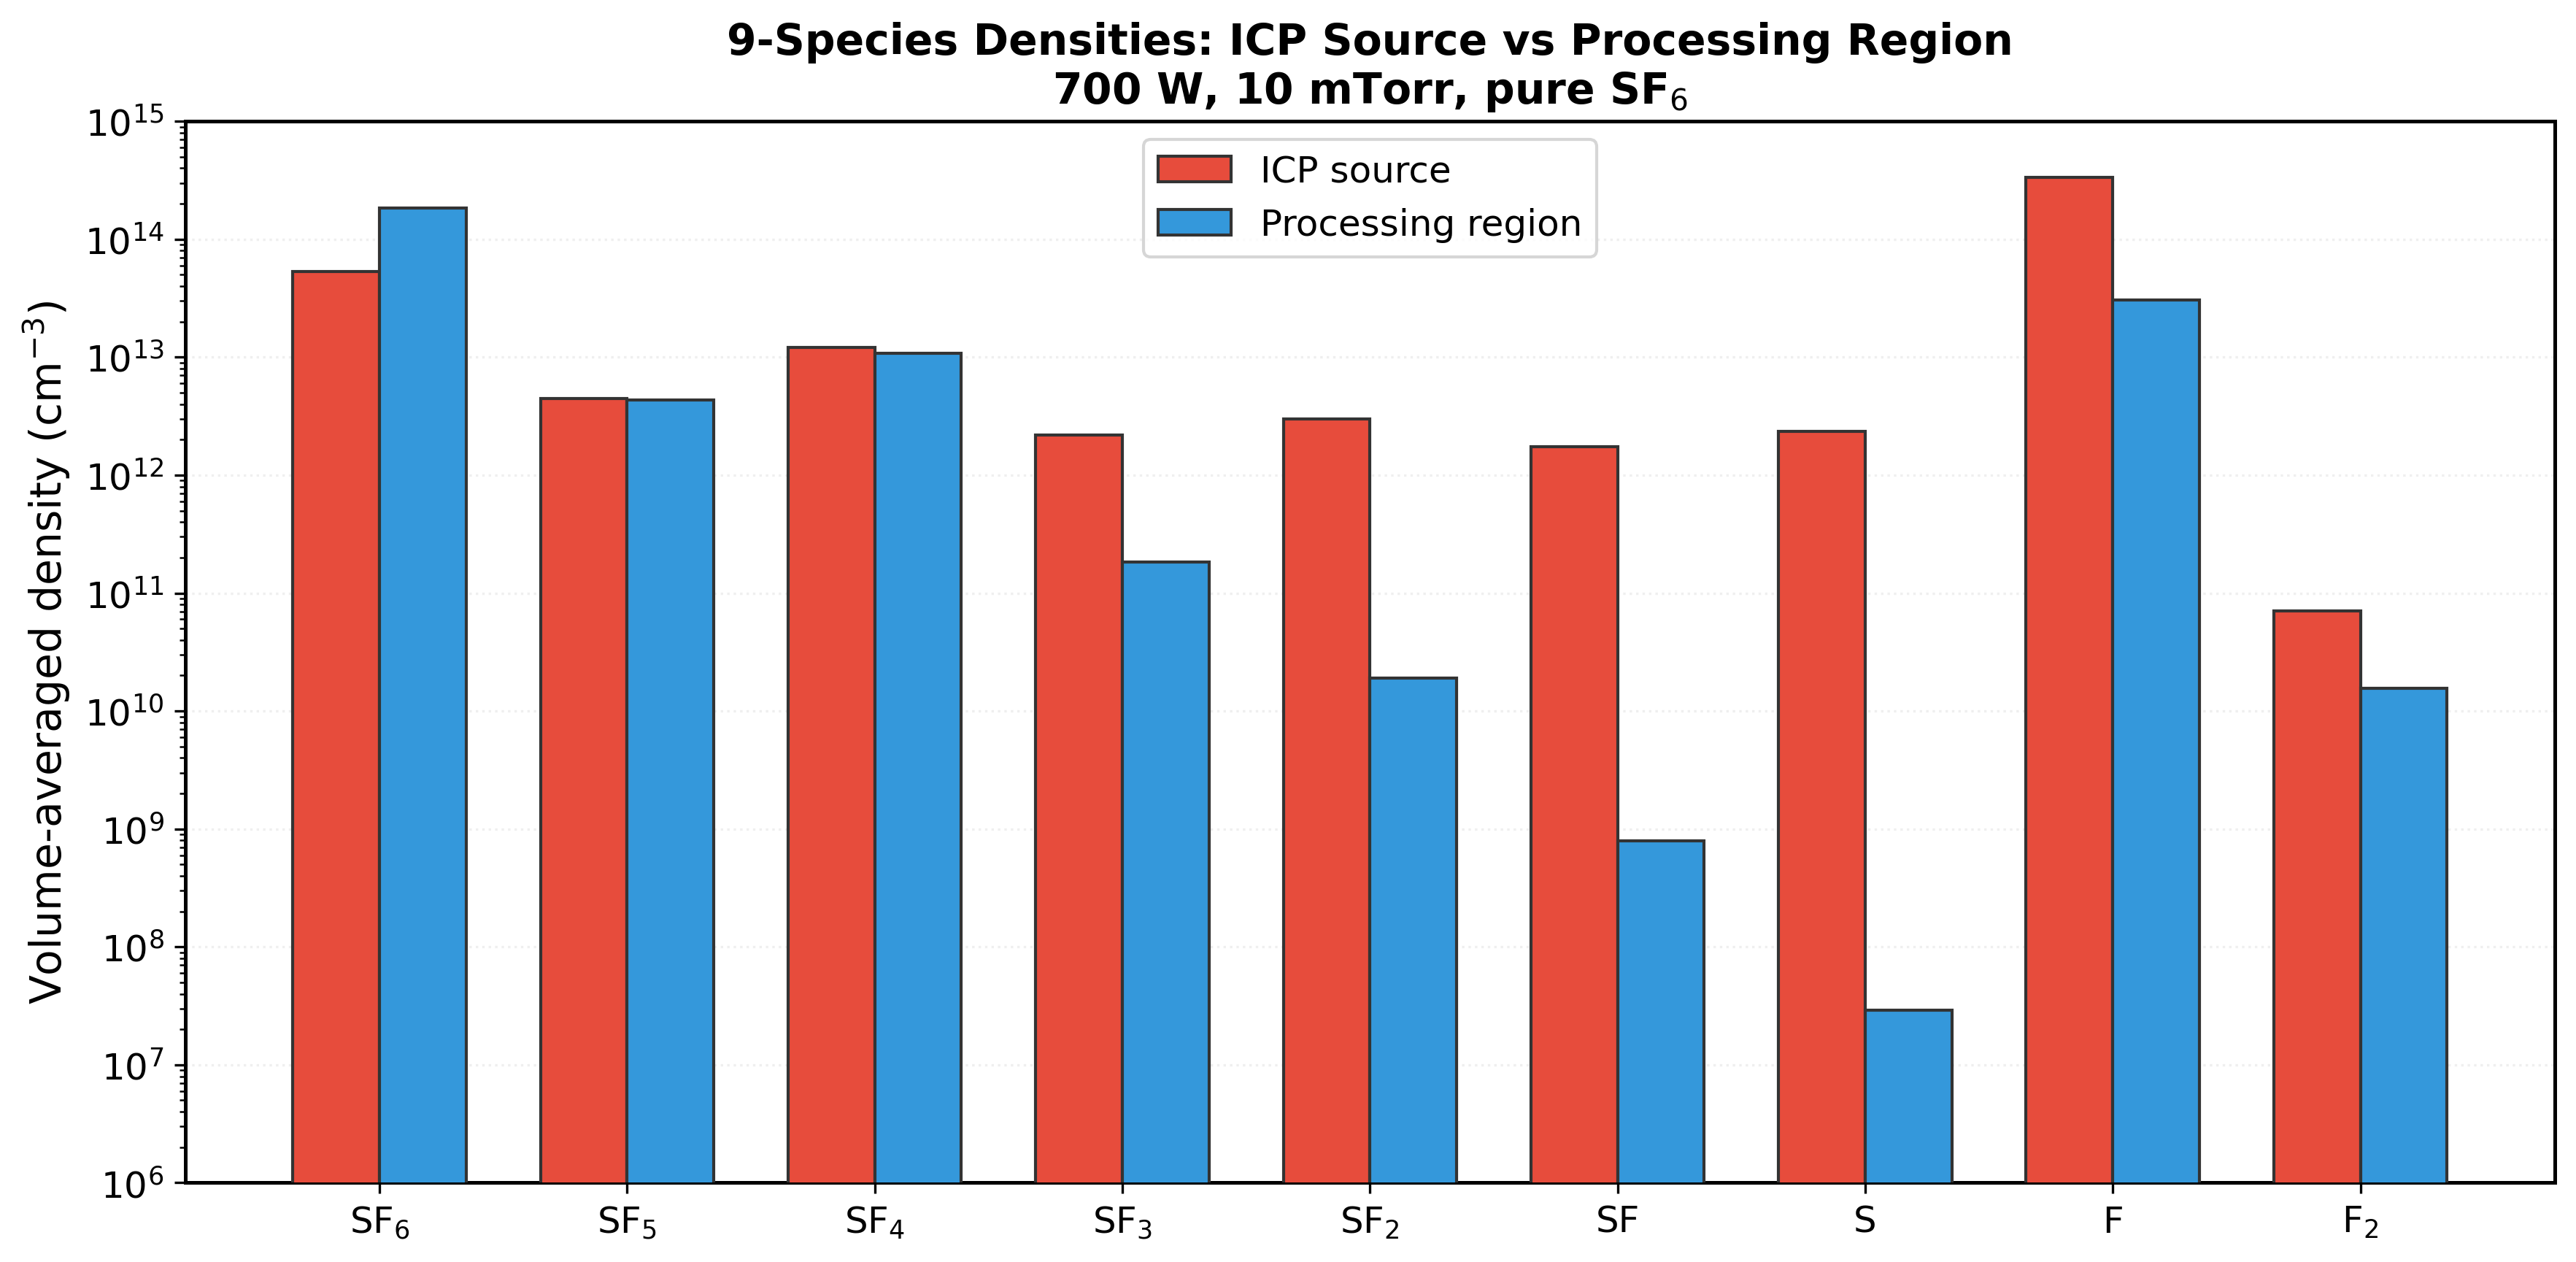
\includegraphics[width=0.65\textwidth]{multispecies_bars.png}
  \caption{Volume-averaged species densities comparing neutral and
           charged species abundances.  SF\textsubscript{6} and F
           dominate the neutral inventory; electrons and
           SF\textsubscript{5}\textsuperscript{$-$} are the
           primary charge carriers.}
  \label{fig:bars}
\end{figure}

% ==================================================================
\section{PINN Attempt: A Negative Result}
\label{sec:pinn}

The first direction pursued after validating the solver was to
accelerate it using physics-informed neural networks
(PINNs)~\citep{raissi2019}, which embed the governing PDEs directly
into the training loss.  The idea was attractive: if the network
could learn to satisfy the continuity, drift--diffusion, and energy
equations without labelled data, it would be both fast and
physically consistent.

\subsection{Data-Only Baseline}

As a sanity check, training with data loss alone converges reliably,
achieving a $23{,}000\times$ loss reduction over the training run.
This confirmed that the network architecture and optimiser were
sound, and that any subsequent failure was attributable to the PDE
loss terms.

\subsection{PDE-Constrained Training}

Adding the PDE residual to the loss function causes \textbf{training
to diverge}.  Root-cause analysis identified five interacting failure
modes:

\begin{enumerate}
  \item \textbf{Stiff chemistry:} rate coefficients span 15+ orders
        of magnitude ($\sim 10^{-22}$ to $10^{-7}$~cm$^3$/s),
        creating extreme loss-landscape curvature that defeats
        gradient-based optimisation.
  \item \textbf{Second-derivative instability:} the diffusion operator
        requires second spatial derivatives of the network output,
        amplifying noise in the automatic-differentiation graph and
        producing oscillatory gradients.
  \item \textbf{Axis singularity:} the $1/r$ term in the cylindrical
        divergence diverges at $r = 0$, creating infinite PDE
        residuals on the symmetry axis.
  \item \textbf{Coupled energy equation:} the electron temperature
        couples nonlinearly to all rate coefficients through
        Arrhenius exponentials, creating feedback loops in the PDE
        residual that amplify small $T_e$ errors.
  \item \textbf{Multi-scale loss:} the PDE residuals for different
        species differ by orders of magnitude (e.g., electron
        continuity vs.\ neutral diffusion), making balanced
        gradient descent infeasible with standard weighting.
\end{enumerate}

These findings constitute a \textbf{clear negative result}: PINNs in
their standard form are not suitable for multi-species,
stiff-chemistry plasma models in cylindrical geometry.  This failure
motivated the pivot to purely supervised surrogate training, which is
the subject of the following sections.

% ==================================================================
\section{Surrogate Development: v1 through v4}
\label{sec:surrogate}

Having established that PINNs diverge, we turned to a data-driven
supervised surrogate.  The development progressed through four
generations, each addressing a specific deficiency identified in the
previous version.

\subsection{Problem Formulation}

The surrogate is a feedforward neural network
$f_\theta : \mathbb{R}^5 \to \mathbb{R}^2$ mapping
\begin{equation}
  (r,\, z,\, P_{\text{rf}},\, p,\, x_{\text{Ar}})
  \;\longmapsto\;
  \bigl(\log_{10} n_{\text{F}},\;
         \log_{10} n_{\text{SF}_6}\bigr).
  \label{eq:surrogate_map}
\end{equation}
Working in log-density space compresses the dynamic range and
naturally enforces positivity.

\subsection{Input Features: Fourier Encoding}

The five raw inputs are augmented with random Fourier features:
\begin{equation}
  \phi(\mathbf{x}) =
  \bigl[\cos(2\pi \mathbf{B}\mathbf{x}),\;
         \sin(2\pi \mathbf{B}\mathbf{x})\bigr],
  \label{eq:fourier}
\end{equation}
where $\mathbf{B} \in \mathbb{R}^{64 \times 5}$ is sampled from
$\mathcal{N}(0, \sigma^2)$ with $\sigma = 3.0$ and held fixed during
training.  This produces a 128-dimensional feature vector that
allows the MLP to represent high-frequency spatial structure
without requiring excessive depth.

\subsection{Surrogate Progression}

Table~\ref{tab:progression} summarises the four generations.

\begin{table}[H]
  \centering
  \caption{Surrogate development progression.  Each version
           addresses a specific deficiency of its predecessor.}
  \label{tab:progression}
  \begin{tabular}{lcl}
    \toprule
    Version & nF RMSE & Key improvement \\
    \midrule
    v1 & 0.133 & Initial MLP + Fourier features \\
    v2 & 0.111 & Data enrichment (more operating points) \\
    v3 & 0.023 & Physics regularisation (smoothness, bounds) \\
    v4 & 0.003 & Output-bias initialisation + ensemble UQ \\
    \bottomrule
  \end{tabular}
\end{table}

The jump from v2 to v3 (0.111 $\to$ 0.023, a $4.8\times$ reduction)
came from adding physics-based regularisation terms.  The further jump
from v3 to v4 (0.023 $\to$ 0.003, a $7.7\times$ reduction) came
primarily from output-bias initialisation, as confirmed by the
ablation study in Section~\ref{sec:ablation}.  Together these
represent a $44\times$ improvement from v1 to v4.

The v4 surrogate achieves a $531\times$ speedup over the legacy
solver (\SI{14.6}{\milli\second} vs.\ \SI{7.76}{\second}).

\subsection{Physics-Based Regularisation}

Three regularisation terms are added to the MSE data loss:

\paragraph{Smoothness penalty.}
Penalises large spatial gradients to suppress unphysical oscillations:
\begin{equation}
  \mathcal{L}_{\text{smooth}}
  = \lambda_{\text{smooth}}
    \left\langle
      \left|\frac{\partial \hat{y}}{\partial r}\right|^2
      + \left|\frac{\partial \hat{y}}{\partial z}\right|^2
    \right\rangle,
  \quad \lambda_{\text{smooth}} = 5 \times 10^{-4}.
  \label{eq:smooth}
\end{equation}

\paragraph{Bounded-density penalty.}
Penalises predictions outside the physically plausible range:
\begin{equation}
  \mathcal{L}_{\text{bound}}
  = \lambda_{\text{bound}}
    \left\langle
      \max(0,\, \hat{y} - y_{\max})^2
      + \max(0,\, y_{\min} - \hat{y})^2
    \right\rangle,
  \quad \lambda_{\text{bound}} = 1 \times 10^{-3}.
  \label{eq:bound}
\end{equation}

\paragraph{Wafer-smoothness penalty.}
An additional smoothness penalty specific to the wafer plane:
\begin{equation}
  \mathcal{L}_{\text{wafer}}
  = \lambda_{\text{wafer}}
    \left\langle
      \left|\frac{\partial \hat{y}}{\partial r}\right|^2
      \bigg|_{z = z_{\text{wafer}}}
    \right\rangle,
  \quad \lambda_{\text{wafer}} = 2 \times 10^{-4}.
  \label{eq:wafer_smooth}
\end{equation}

\subsection{Output Bias Initialisation}

The final bias of each head is initialised to the log-mean of the
corresponding species density across the training set:
\begin{equation}
  b_{\text{F}}^{(0)} = 19.8, \qquad
  b_{\text{SF}_6}^{(0)} = 20.0.
  \label{eq:bias_init}
\end{equation}
This ensures that the network output starts near the correct order of
magnitude ($\sim 10^{19}$--$10^{20}\;\si{\per\cubic\metre}$),
dramatically accelerating convergence.  As shown in
Section~\ref{sec:ablation}, this single design choice accounts for
roughly 74\% of the total RMSE reduction in the LXCat ablation.

% ==================================================================
\section{LXCat Cross-Section Integration}
\label{sec:lxcat}

\subsection{Motivation and Implementation}

The legacy solver uses tabulated electron-impact cross sections.
To improve traceability, we integrated the Biagi-v10.6
dataset~\citep{biagi} from the LXCat platform~\citep{lxcat}.  The
Biagi cross sections were parsed from the LXCat database format, and
Maxwellian-averaged rate coefficients were computed as functions of
electron temperature.  The solver was modified to support a
\texttt{rate\_mode='lxcat'} flag that selects between the legacy
tabulated rates and the new LXCat-derived rates.

\begin{figure}[H]
  \centering
  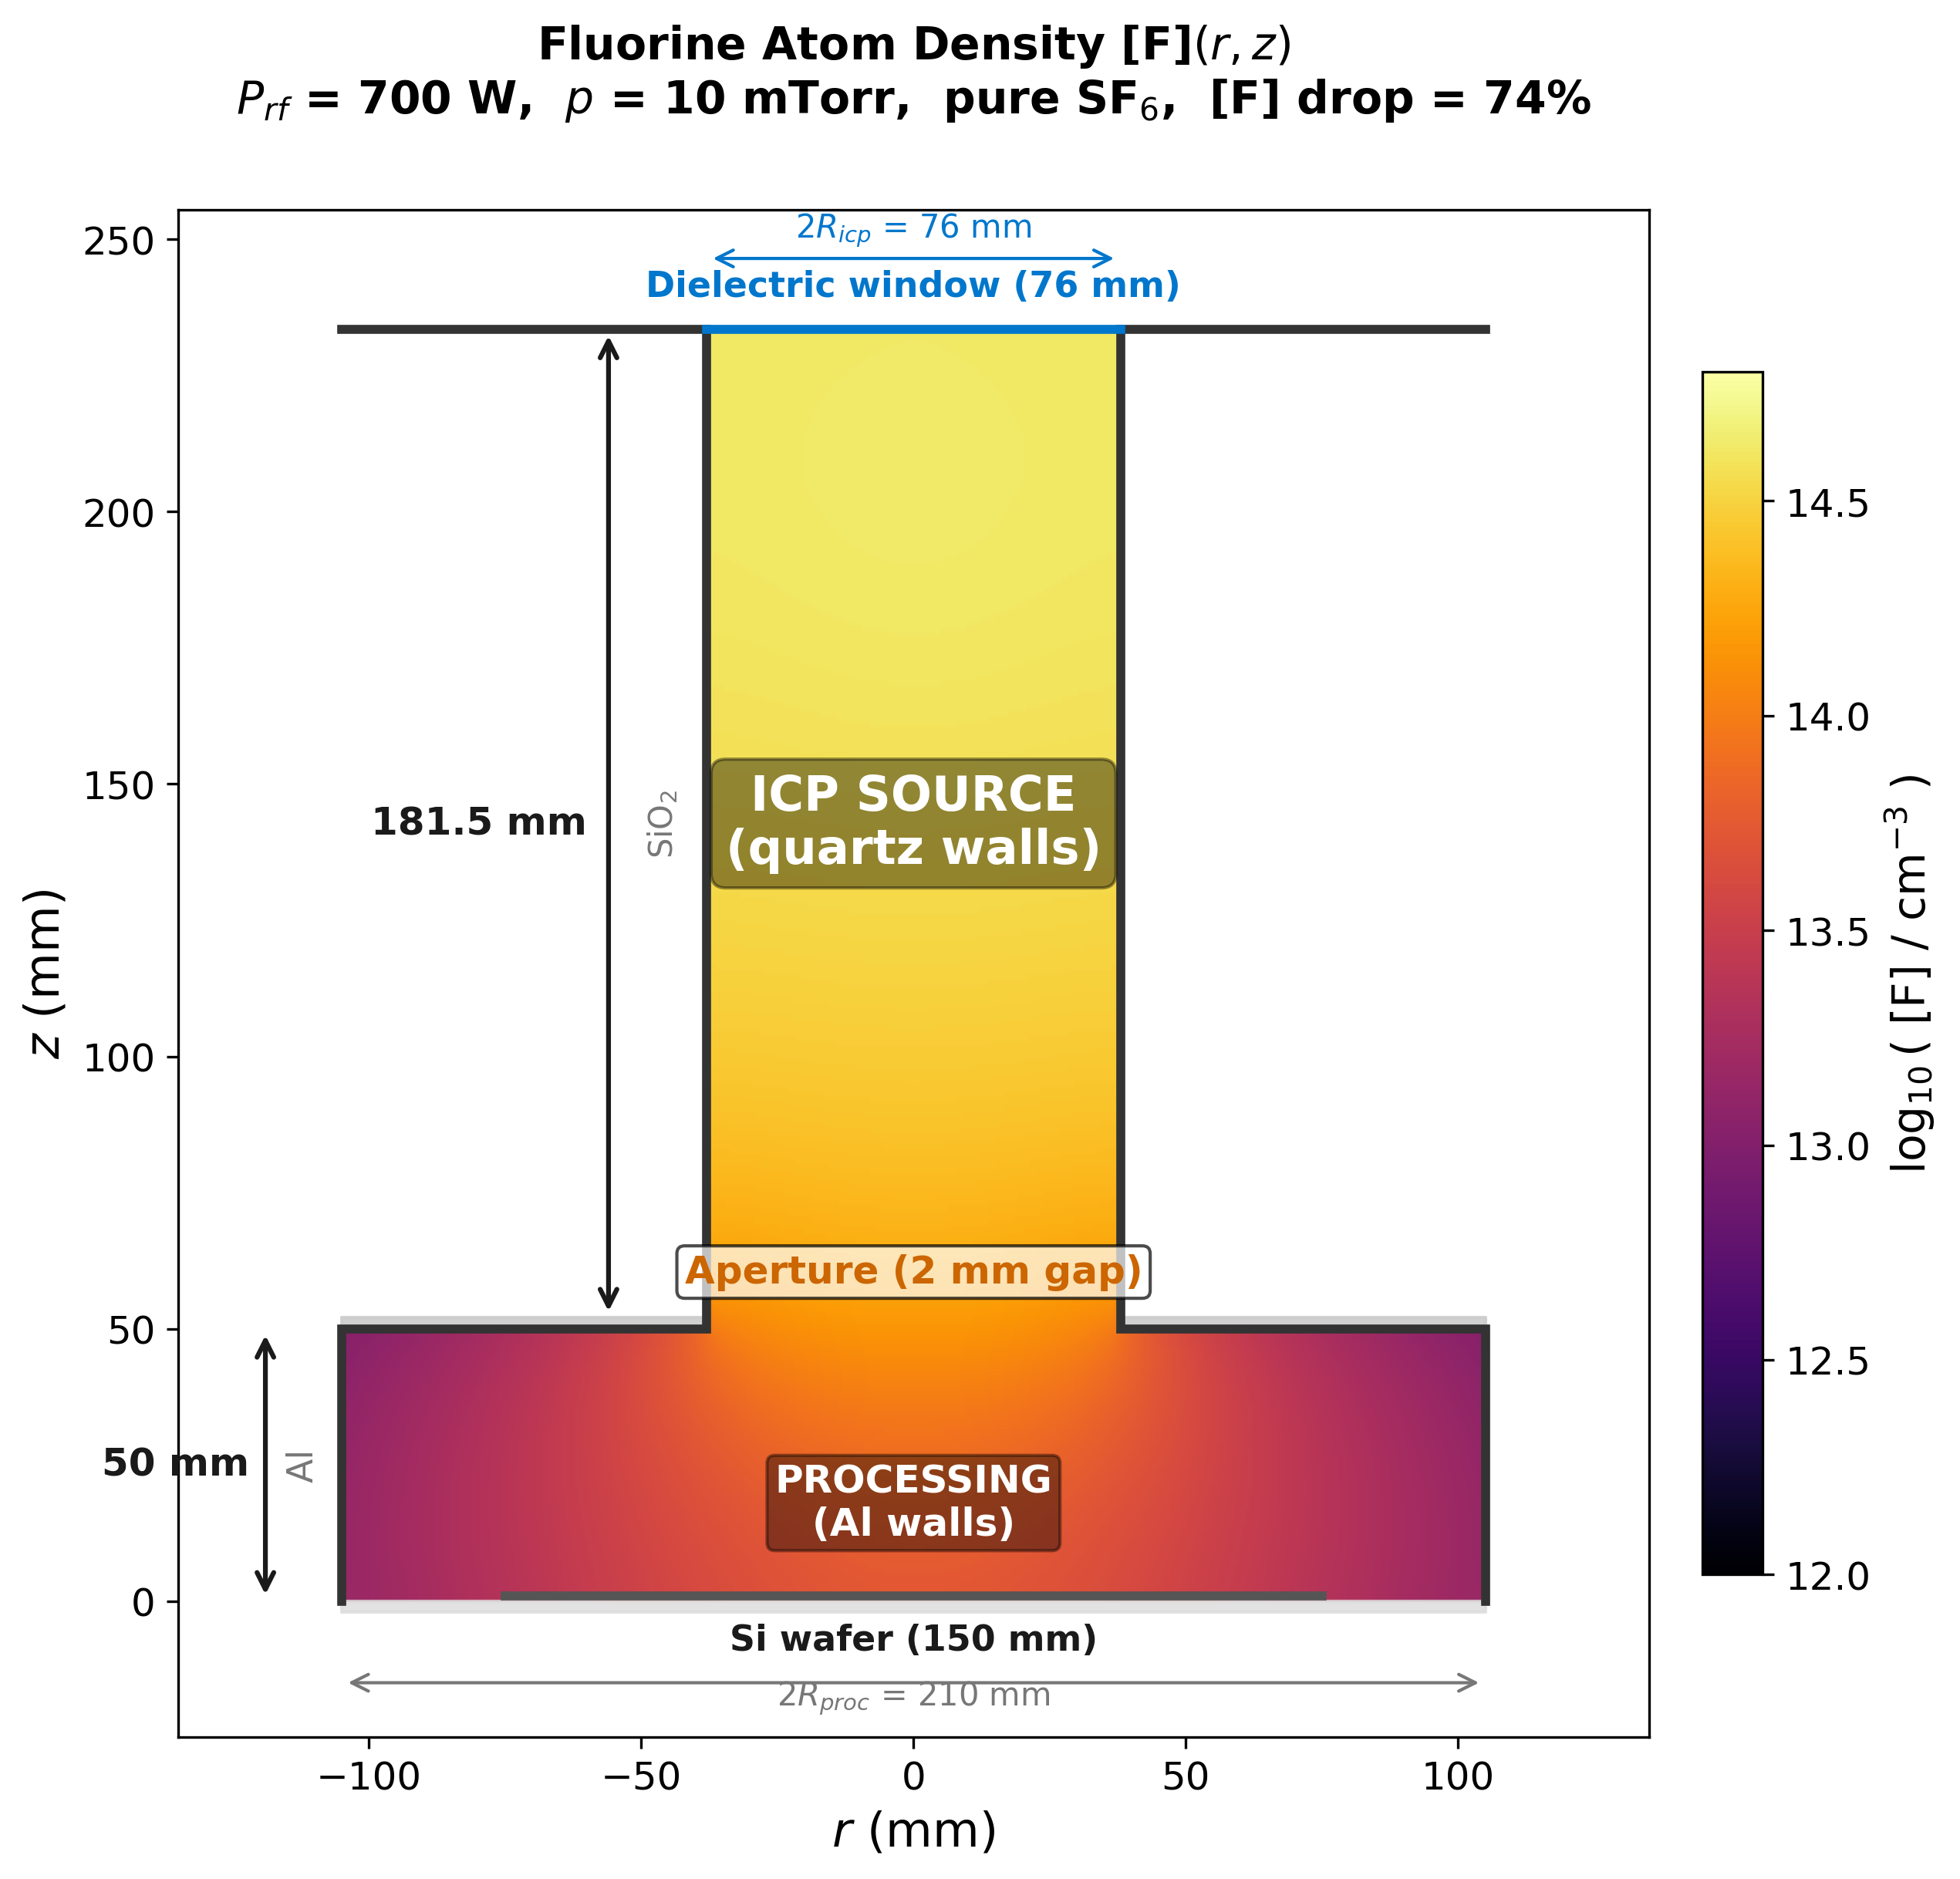
\includegraphics[width=0.65\textwidth]{cross_sections.png}
  \caption{Electron-impact cross sections for key SF\textsubscript{6}
           processes from the Biagi-v10.6 dataset.  The dominant channels
           are dissociative attachment and vibrational excitation at
           low electron energies, and ionisation at higher energies.}
  \label{fig:cross_sections}
\end{figure}

\subsection{Rate Coefficient Comparison}

Figure~\ref{fig:rate_comparison} compares selected rate coefficients
between the legacy and LXCat sets.  The differences are most
pronounced for dissociative attachment at low $E/N$, which is the
dominant source of F atoms.

\begin{figure}[H]
  \centering
  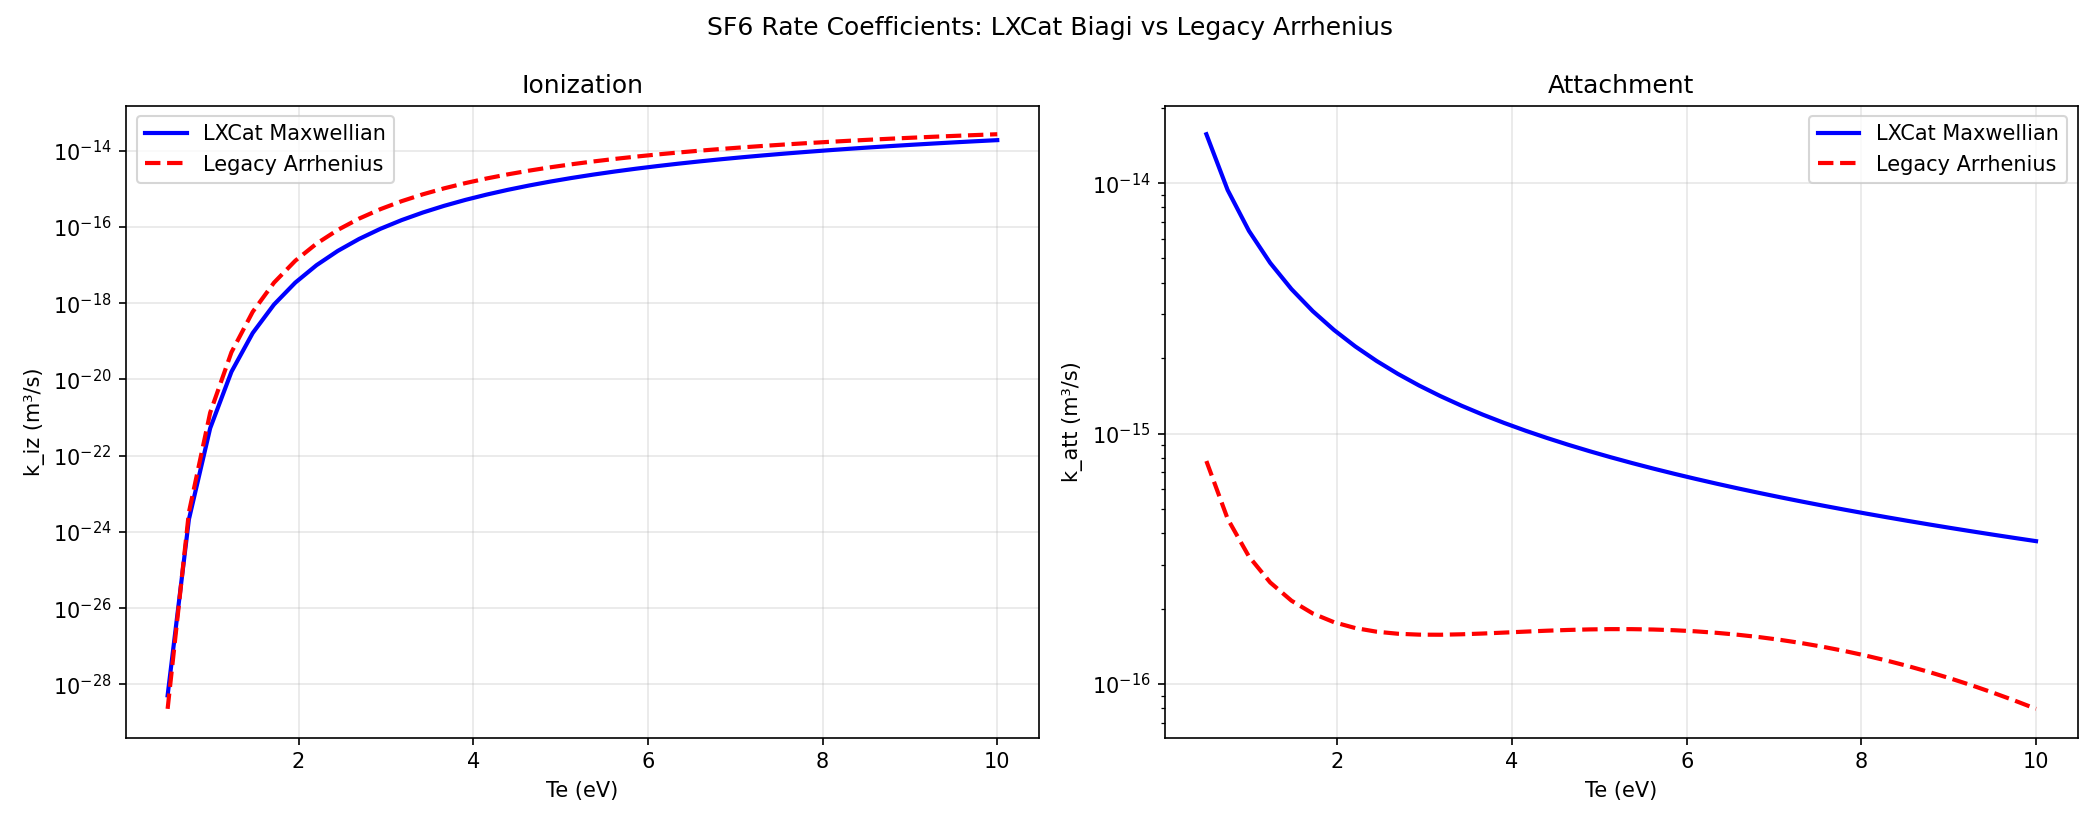
\includegraphics[width=0.65\textwidth]{lxcat_rate_comparison.png}
  \caption{Comparison of selected electron-impact rate coefficients
           computed from legacy tabulated cross sections versus the
           LXCat/Biagi-v10.6 set.  Differences are most pronounced for
           dissociative attachment at low $E/N$.}
  \label{fig:rate_comparison}
\end{figure}

\subsection{Physics Impact}

The LXCat solver produces dramatically different plasma parameters at
the same operating conditions:
\begin{itemize}
  \item \textbf{Electron temperature:} $T_e$ increases by \textbf{56\%}.
        The Biagi cross sections have lower inelastic loss rates at the
        relevant energies, requiring a higher $T_e$ to sustain the
        discharge.
  \item \textbf{Electron density:} $n_e$ decreases by \textbf{69\%},
        consistent with the higher $T_e$ (fewer electrons needed at
        higher mean energy to maintain ionisation balance).
  \item \textbf{F density:} unchanged within numerical accuracy.
        The dissociation rate adjusts to compensate for the $T_e$ and
        $n_e$ shifts.
\end{itemize}
The invariance of F density despite large shifts in $T_e$ and $n_e$
is a surprising and physically meaningful result: it suggests that
the F density is controlled primarily by transport (diffusion through
the aperture and wall recombination) rather than by the details of
electron-impact kinetics.

Figure~\ref{fig:lxcat_wafer} shows the radial F density profile at
the wafer from the LXCat solver.

\begin{figure}[H]
  \centering
  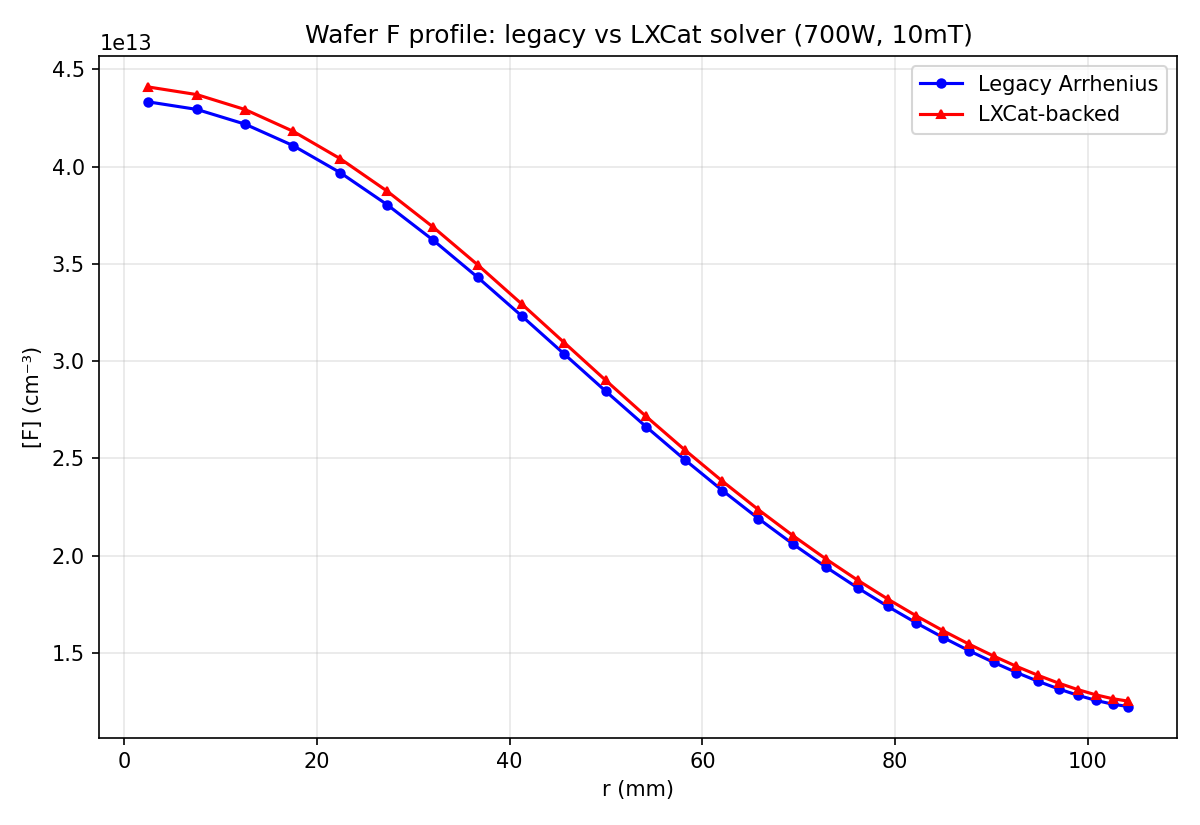
\includegraphics[width=0.6\textwidth]{lxcat_solver_wafer_profile.png}
  \caption{Radial F density profile at the wafer predicted by the
           LXCat solver.  The profile shape is similar to the legacy
           solver; absolute densities are nearly identical despite
           the large $T_e$ and $n_e$ shifts.}
  \label{fig:lxcat_wafer}
\end{figure}

\subsection{Dataset Diagnosis: Recipe, Not Physics}
\label{sec:dataset_diagnosis}

When the v4 training recipe was applied to LXCat data, the initial
RMSE was $3.85\times$ worse than on legacy data.  A natural hypothesis
was that the LXCat data are intrinsically harder to learn.  We tested
this by comparing the statistical properties of the two datasets:
\begin{itemize}
  \item Log-density standard deviation ratio: $0.99\times$.
  \item Gradient P90 ratio: $0.99\times$.
  \item Correlation shift: $< 0.003$.
\end{itemize}
The two datasets are \textbf{statistically identical} in difficulty.
The $3.85\times$ RMSE gap was entirely attributable to the training
recipe (architecture, initialisation, regularisation), not to any
difference in the underlying data distributions.  This finding
motivated the architecture sweep described in the next section.

% ==================================================================
\section{Architecture Sweep}
\label{sec:arch_sweep}

Having established that the performance gap was a recipe problem, we
conducted a controlled architecture sweep to find the best topology
for the LXCat dataset.

\subsection{Experimental Design}

Seven architectures (E0--E6) were evaluated, each trained with three
random seeds on the LXCat dataset under identical training budgets.
Table~\ref{tab:arch_sweep} reports the mean and standard deviation
of the normalised F-density RMSE.

\begin{table}[H]
  \centering
  \caption{Architecture sweep results (LXCat dataset, 3 seeds each).
           RMSE values are normalised.}
  \label{tab:arch_sweep}
  \begin{tabular}{llcc}
    \toprule
    ID & Architecture & nF RMSE & $\pm\,1\sigma$ \\
    \midrule
    E0 & Baseline (no reg, 1500 ep)
       & 0.02022 & 0.00275 \\
    E1 & V4 recipe (reg + bias + 2000 ep)
       & 0.00570 & 0.00074 \\
    E2 & Wider/deeper ($6\times256$ + reg)
       & 0.00573 & 0.00102 \\
    E3 & \textbf{Separate heads} (trunk + heads + reg)
       & \textbf{0.00410} & \textbf{0.00021} \\
    E4 & Residual (res blocks + reg)
       & 0.00449 & 0.00028 \\
    E5 & Enhanced features (10 inputs + reg)
       & 0.01060 & 0.00118 \\
    E6 & Huber loss (Huber + reg)
       & 0.00572 & 0.00042 \\
    \bottomrule
  \end{tabular}
\end{table}

\subsection{Analysis}

\textbf{E3\_separate\_heads} achieves the lowest mean RMSE (0.00410)
with the smallest seed-to-seed variance ($\sigma = 0.00021$),
indicating both accuracy and training stability.  Key observations:
\begin{itemize}
  \item E4 (residual) is a close second but with a wider seed-to-seed
        spread, making it less reliable.
  \item Simply making the network wider and deeper (E2) provides no
        benefit over the v4 recipe (E1), confirming that capacity is
        not the bottleneck.
  \item Expanding the feature set (E5) \emph{hurts} performance
        ($2.6\times$ worse than E3), likely due to the curse of
        dimensionality on the modest training set.
  \item Huber loss (E6) offers no advantage over MSE in this
        application.
\end{itemize}

The single-model E3 nF~RMSE of 0.00410 closes most of the gap to
the legacy v4 surrogate (1.4$\times$), and on nSF\textsubscript{6} the
same architecture delivers best-in-class
$0.00168 \pm 0.00013$, comfortably below the v4 baseline of 0.0027.

\subsection{E3 Architecture}

The winning architecture (Figure~\ref{fig:flowchart}) consists of:
\begin{enumerate}
  \item A \textbf{shared trunk}: 3 hidden layers of width 128 with
        ReLU activations and a skip connection from the Fourier
        features to the trunk output.
  \item \textbf{Two species-specific heads}: each a 2-layer MLP
        with width 64 and ReLU activations, producing a scalar
        output for $\log_{10} n_{\text{F}}$ and
        $\log_{10} n_{\text{SF}_6}$ respectively.
\end{enumerate}
The shared trunk captures common spatial patterns (geometry, power
deposition), while the separate heads specialise to species-specific
chemistry.

\begin{figure}[H]
  \centering
  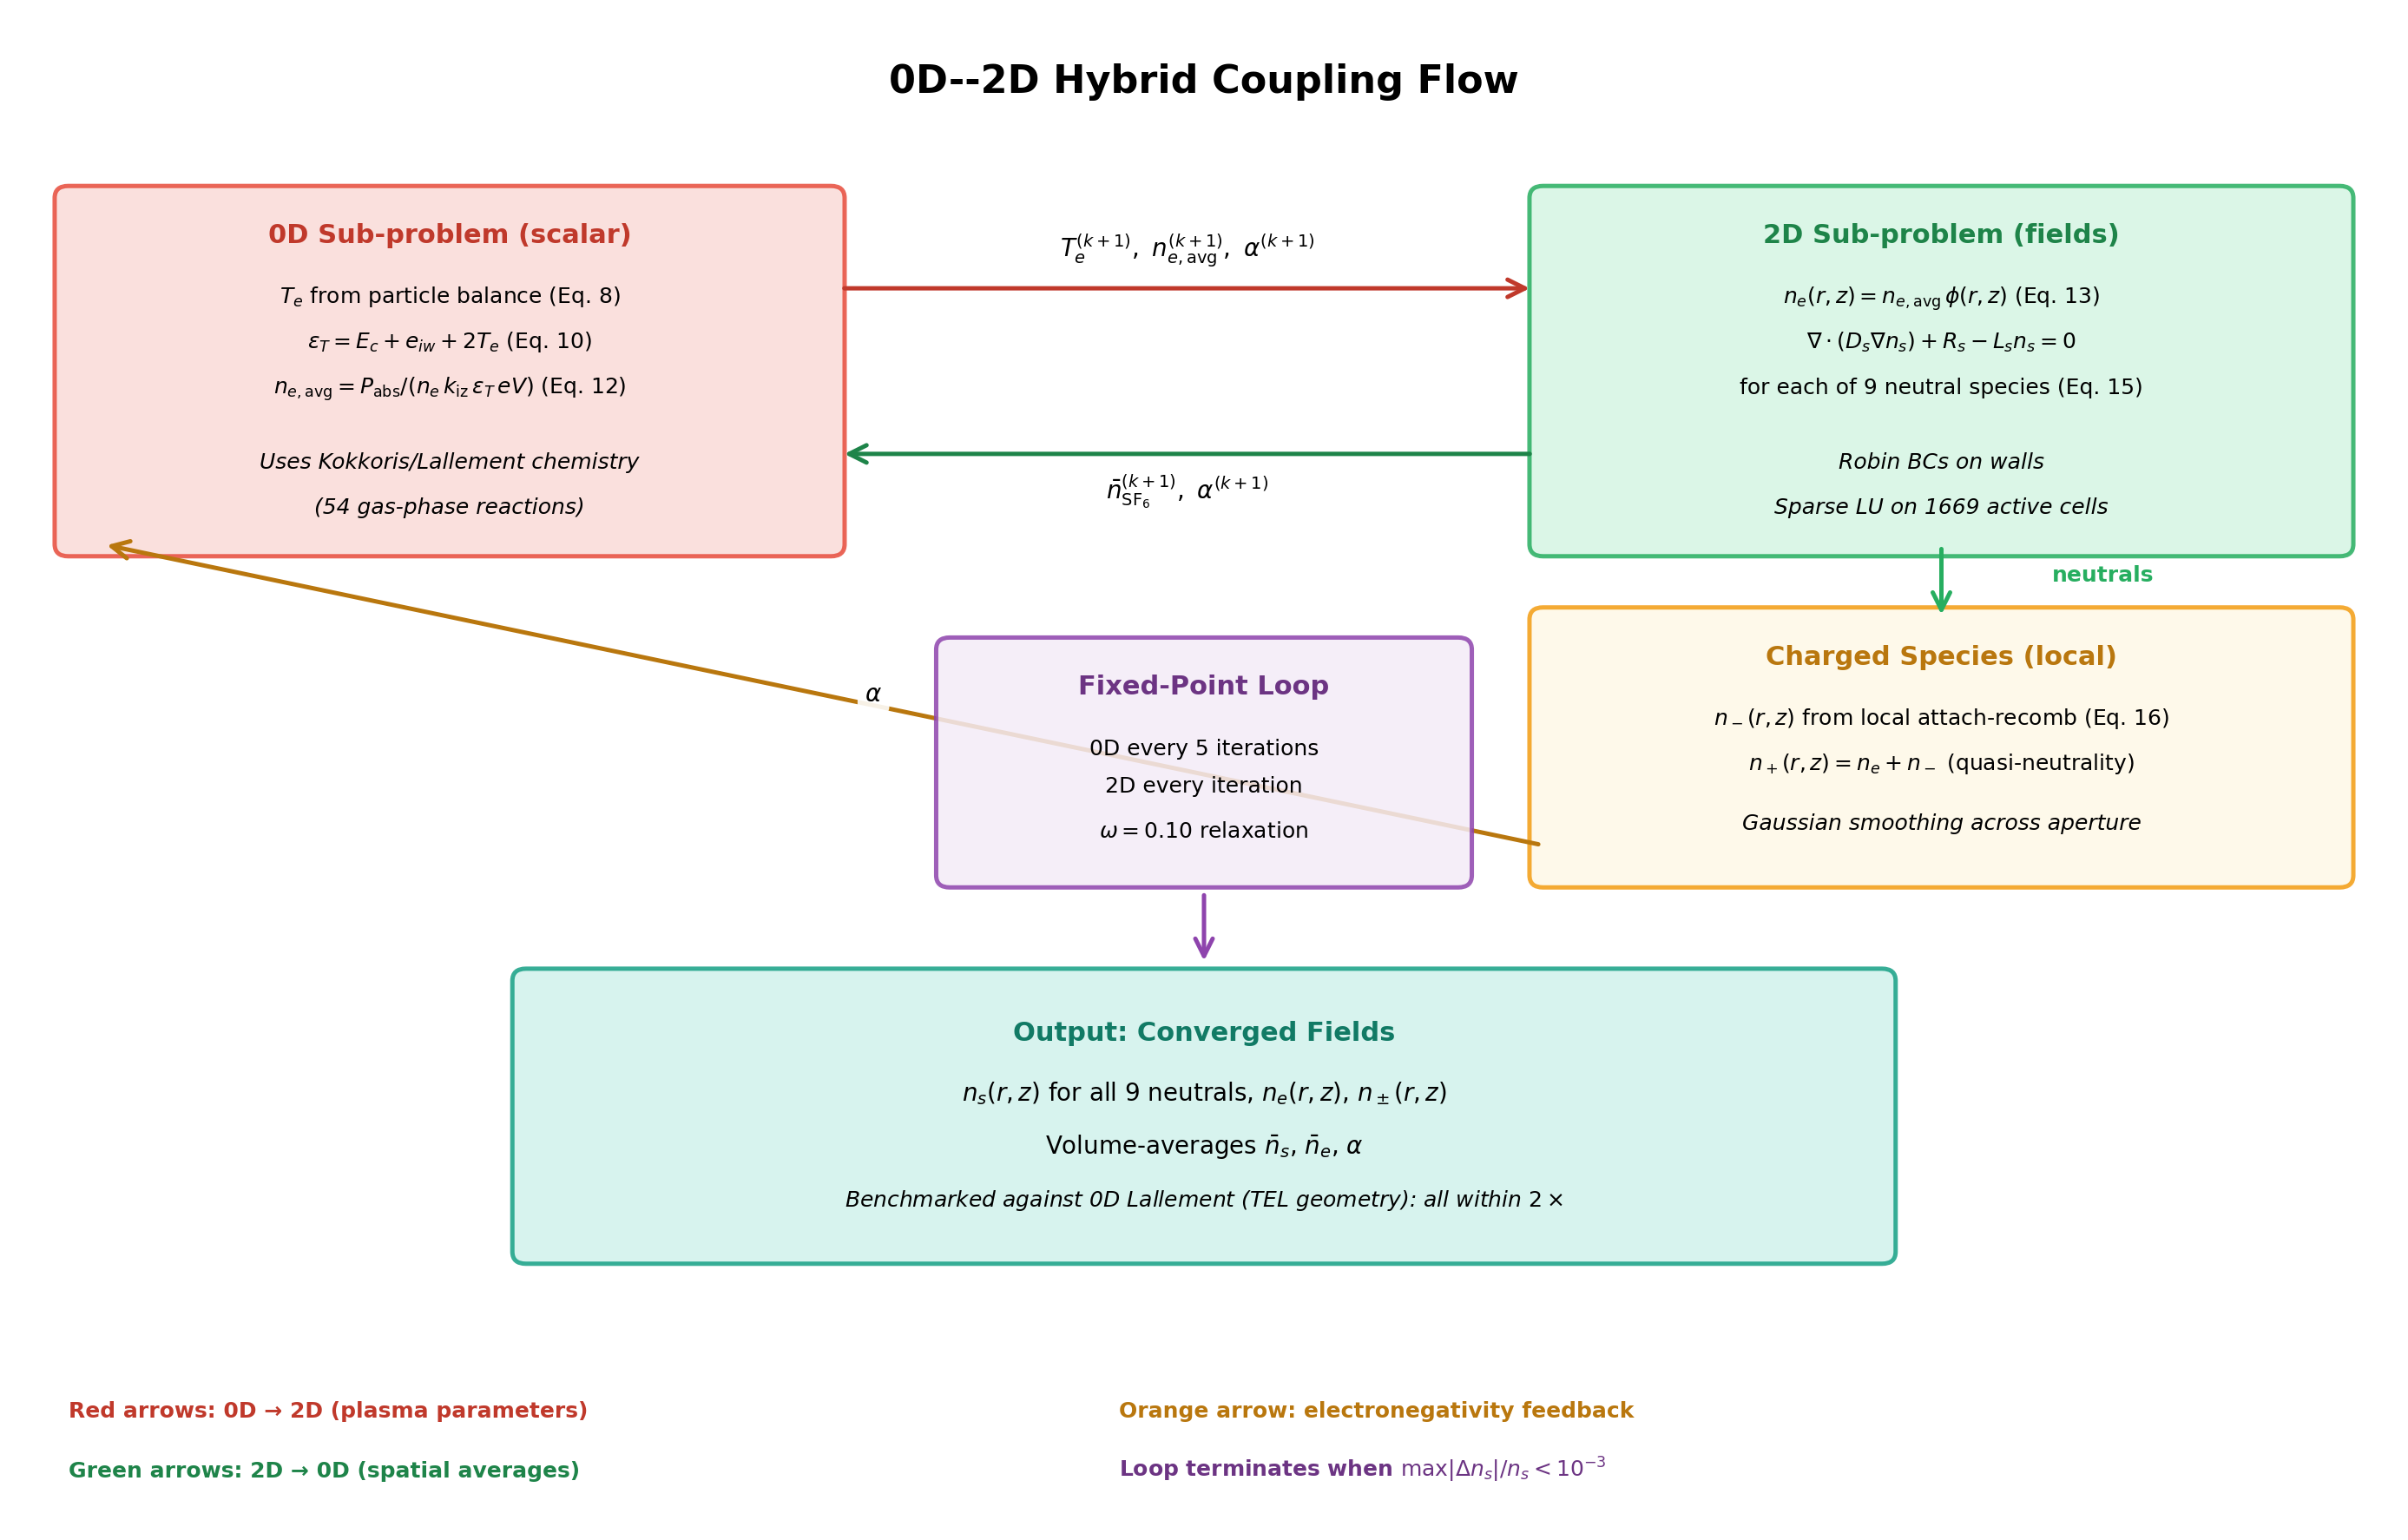
\includegraphics[width=0.55\textwidth]{coupling_flowchart.png}
  \caption{Surrogate architecture (E3\_separate\_heads).  The shared
           trunk receives Fourier-encoded inputs; a skip connection
           concatenates the raw Fourier features with the trunk output
           before feeding species-specific head networks.}
  \label{fig:flowchart}
\end{figure}

% ==================================================================
\section{Ablation Study}
\label{sec:ablation}

To disentangle the contributions of regularisation, bias
initialisation, and extended training, we ran a single-factor ablation
with five configurations (3 seeds each).  Results are in
Table~\ref{tab:ablation}.

\begin{table}[H]
  \centering
  \caption{Ablation study.  Improvement is relative to the ``none''
           baseline (nF RMSE = 0.01941).}
  \label{tab:ablation}
  \begin{tabular}{lcc}
    \toprule
    Configuration & nF RMSE & Improvement \\
    \midrule
    None (baseline)     & 0.01941 & ---   \\
    Bias only           & 0.00511 & +74\% \\
    Regularisation only & 0.01948 & $-0.4$\%\\
    Epochs only (2000)  & 0.01918 & +1\% \\
    All three           & 0.00557 & +71\% \\
    \bottomrule
  \end{tabular}
\end{table}

\subsection{Key Findings}

The ablation reveals a clear hierarchy:

\paragraph{Bias initialisation is the dominant factor.}
Adding output-bias initialisation alone reduces the RMSE from 0.01941
to 0.00511---a 74\% improvement and the only single-factor lever that
moves the result by more than a few percent.  Without this, the
network spends its first hundreds of epochs merely shifting the output
mean from near-zero to the correct order of magnitude ($\sim 10^{19}$--
$10^{20}$~m$^{-3}$), during which time the spatial structure signal
is overwhelmed by the magnitude error.

\paragraph{Regularisation alone is useless.}
Adding smoothness, bounds, and wafer-smoothness penalties without bias
initialisation yields nF RMSE = 0.01948---essentially indistinguishable
from the baseline ($-0.4\%$).  The regularisation constrains the
spatial structure before the network has found the correct magnitude,
neither helping nor hurting convergence in this regime.

\paragraph{Extended training provides essentially no gain.}
Increasing from 1500 to 2000 epochs alone moves nF RMSE from 0.01941
to 0.01918 (a 1\% improvement), confirming that the fundamental
bottleneck is initialisation, not epoch budget.

\paragraph{The ``all three'' configuration is slightly worse than
bias-only.}  nF RMSE = 0.00557 vs.\ 0.00511 for bias-only, because
the regularisation terms slightly increase the data-fit loss.  This
is an acceptable trade-off: the regularised model produces smoother,
more physically plausible spatial profiles despite the marginal RMSE
increase.

% ==================================================================
\section{Production Ensemble}
\label{sec:production}

The winning E3 architecture was retrained as a 5-model ensemble,
achieving:
\begin{align}
  \text{nF RMSE}              &= 0.00381, \label{eq:nf_rmse} \\
  \text{nSF}_6\text{ RMSE}    &= 0.00134. \label{eq:nsf6_rmse}
\end{align}
This is a \textbf{66\% improvement on nF} over the v3 LXCat baseline
(nF~RMSE = 0.0112) and an \textbf{83\% improvement on
nSF\textsubscript{6}} over the same baseline (0.0081).  Against the
legacy surrogate\_v4, the current ensemble matches nF within
$1.31\times$ (0.00381 vs.\ 0.0029) while reducing
nSF\textsubscript{6}~RMSE by $\sim$\textbf{2$\times$} (0.00134
vs.\ 0.0027).  The ensemble was trained with the Adam optimiser and a
cosine-annealing learning-rate schedule for 2000 epochs with a batch
size of 4096.

\subsection{Diagnostics}

Figure~\ref{fig:diagnostics} shows diagnostic plots for both target
species, including residual distributions, spatial error maps, and
per-condition RMSE breakdowns.  The residuals are approximately
Gaussian with no systematic bias.

\begin{figure}[H]
  \centering
  \begin{subfigure}[t]{0.48\textwidth}
    \centering
    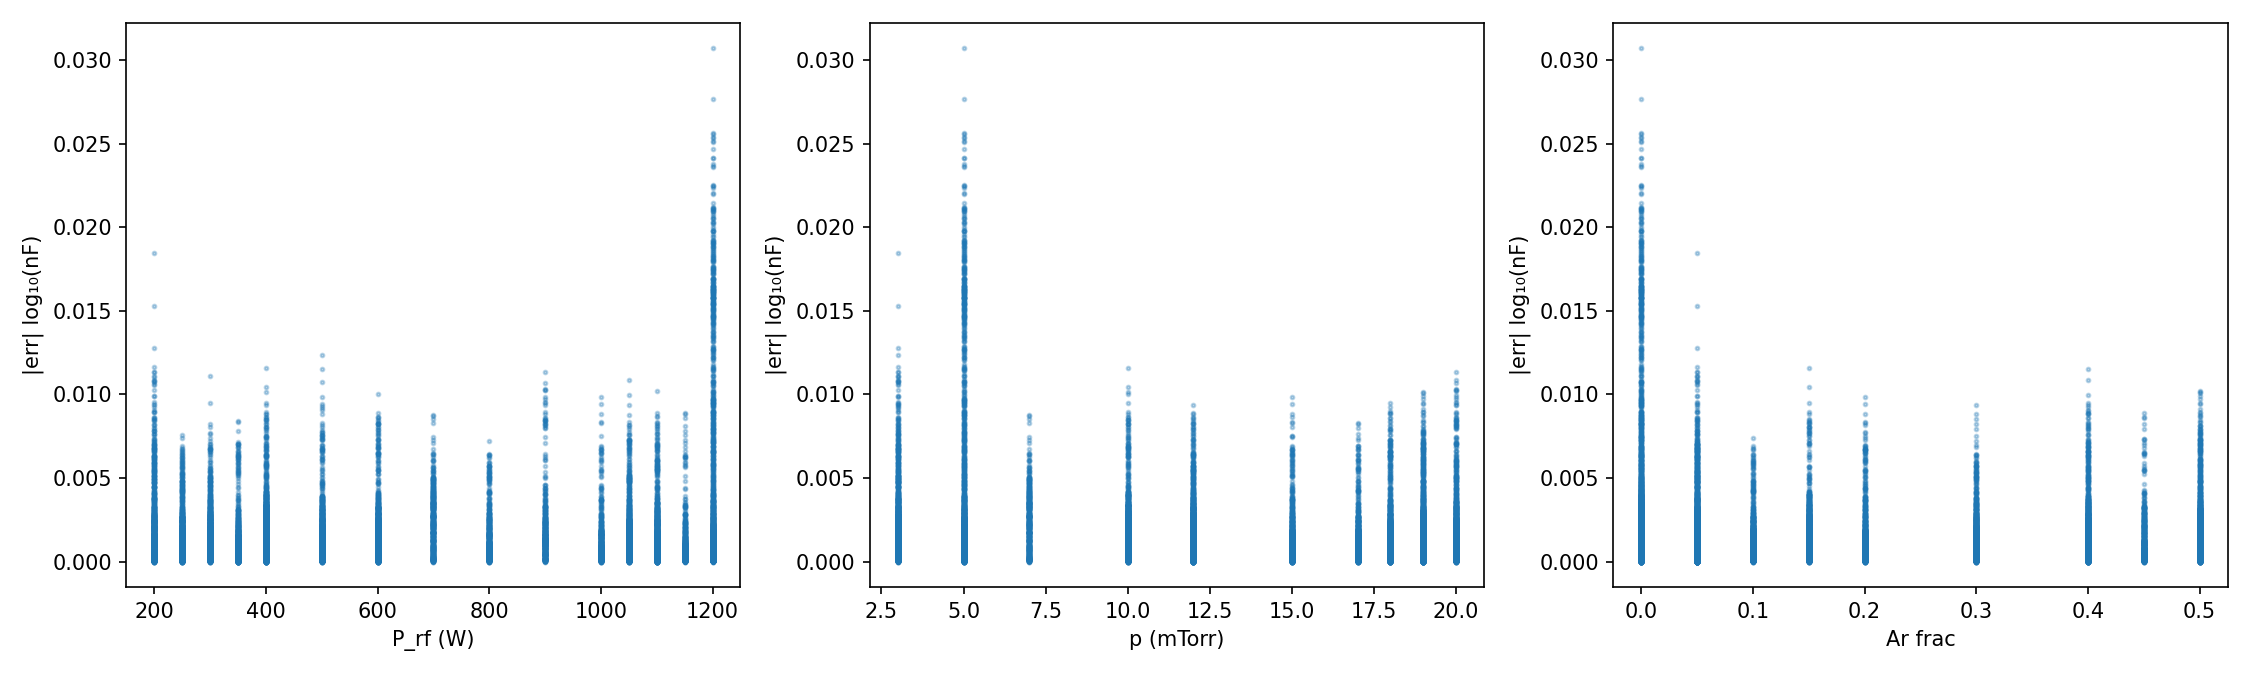
\includegraphics[width=\textwidth]{surrogate_v4_diagnostics_nF.png}
    \caption{F density diagnostics.}
    \label{fig:diag_nF}
  \end{subfigure}
  \hfill
  \begin{subfigure}[t]{0.48\textwidth}
    \centering
    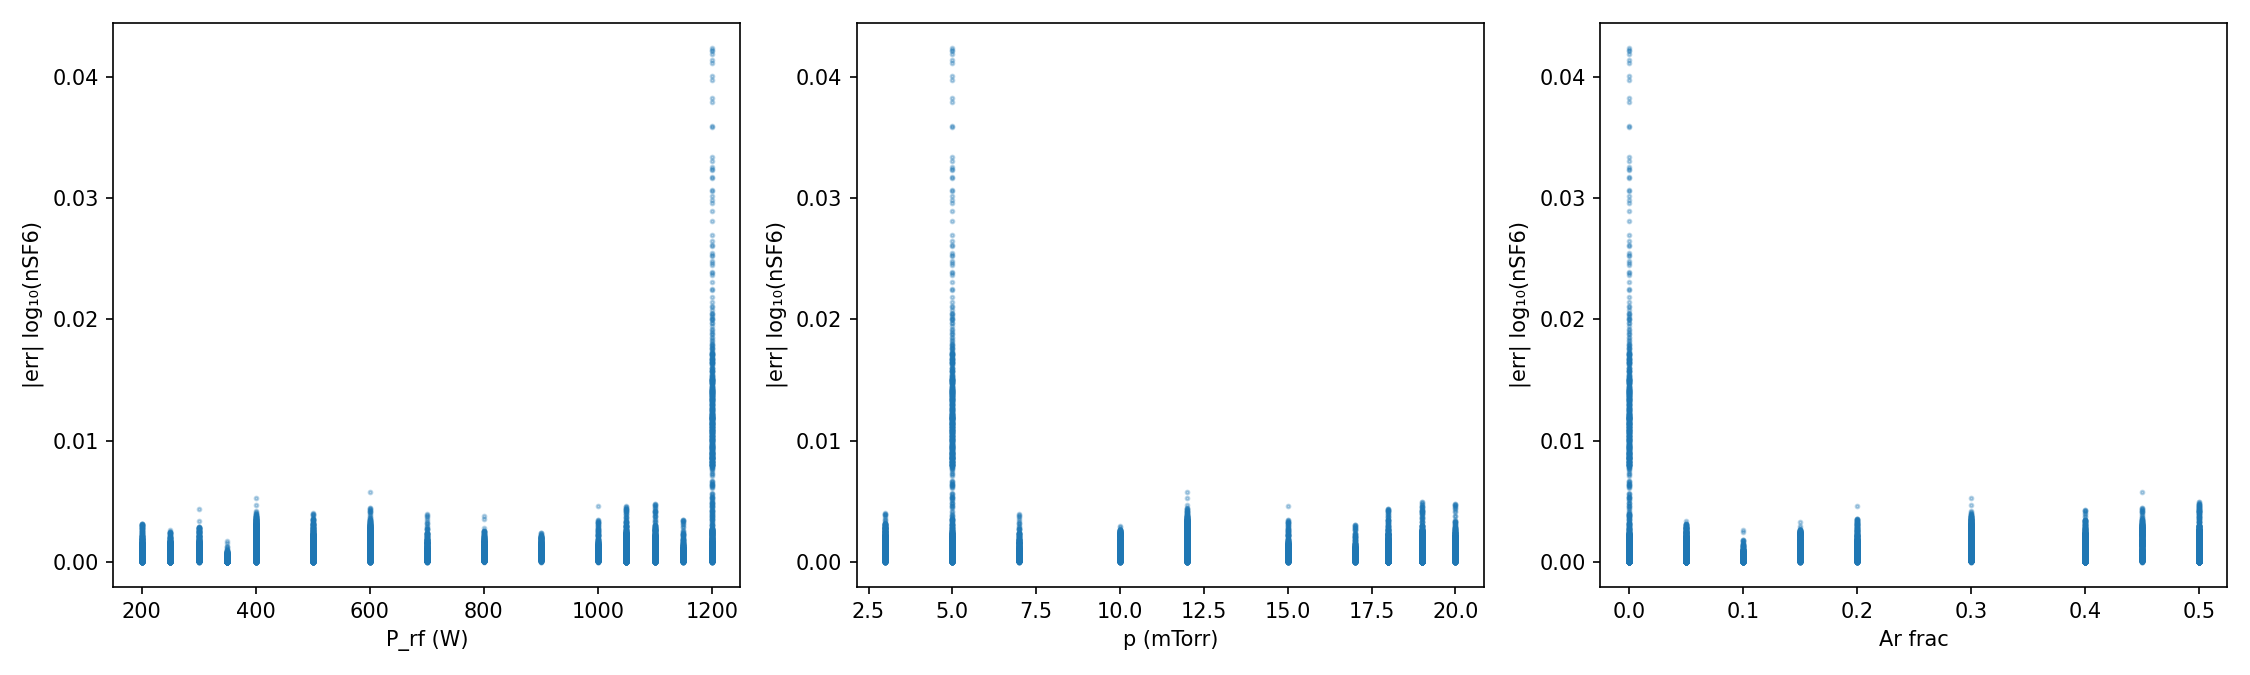
\includegraphics[width=\textwidth]{surrogate_v4_diagnostics_nSF6.png}
    \caption{SF\textsubscript{6} density diagnostics.}
    \label{fig:diag_nSF6}
  \end{subfigure}
  \caption{Surrogate diagnostic plots showing residual distributions,
           spatial error maps, and per-condition RMSE for both target
           species.}
  \label{fig:diagnostics}
\end{figure}

\subsection{Predicted vs.\ True}

Figure~\ref{fig:pred_vs_true} confirms that predictions cluster
tightly around the identity line across four orders of magnitude.

\begin{figure}[H]
  \centering
  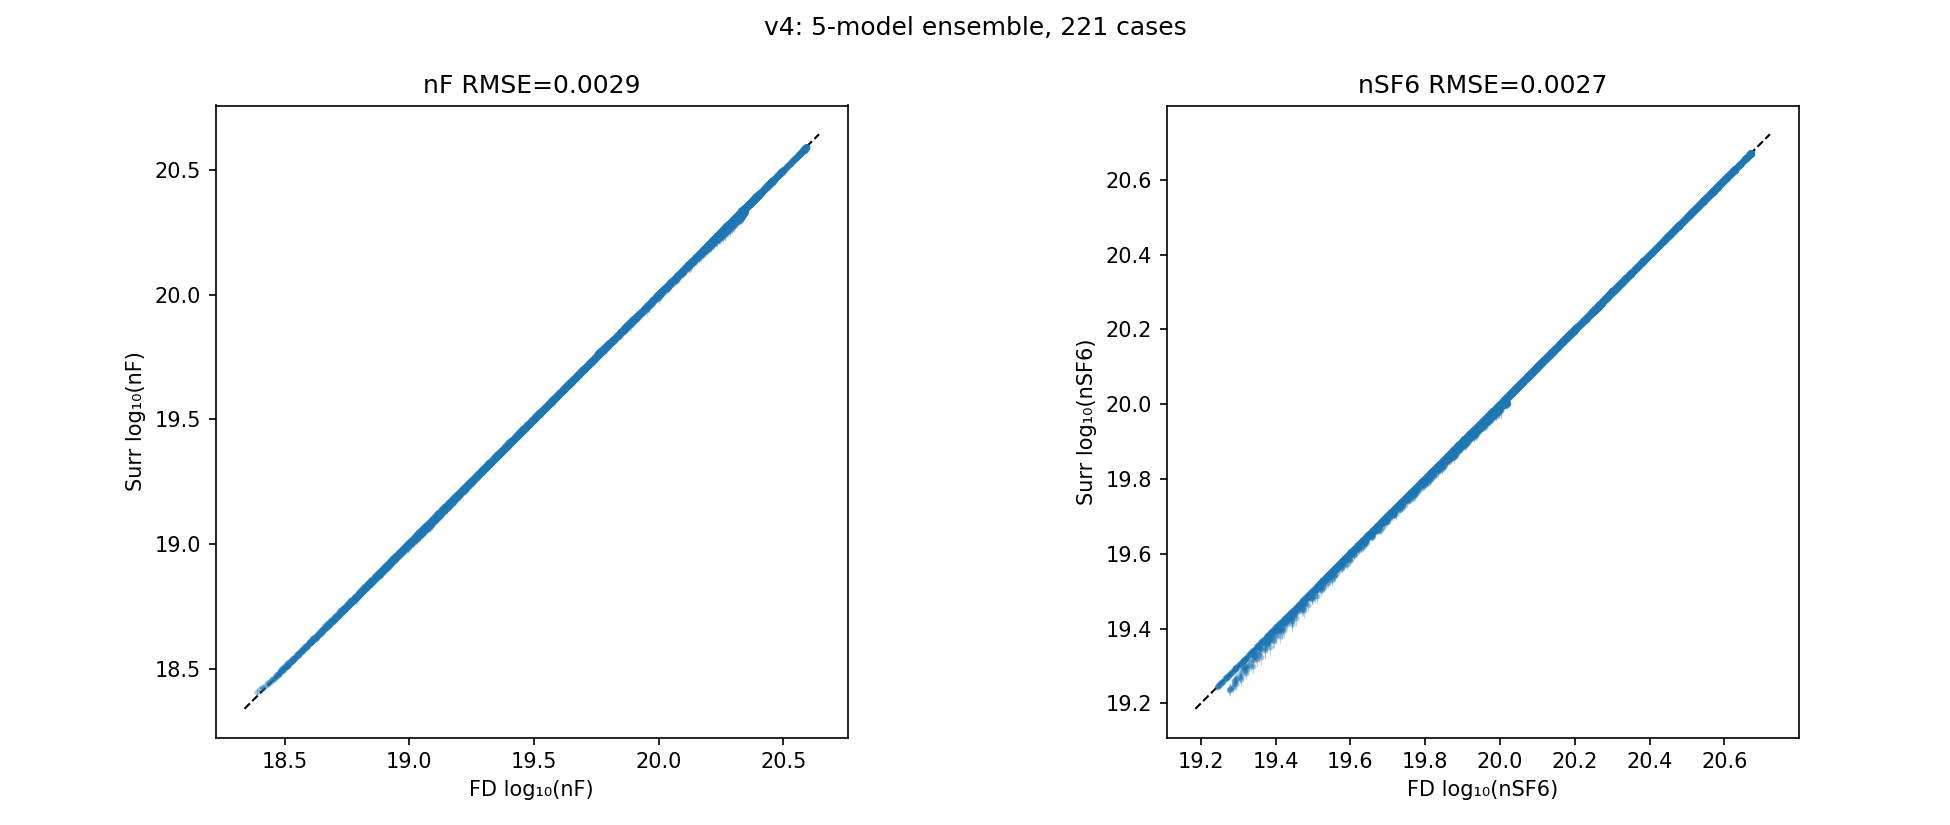
\includegraphics[width=0.6\textwidth]{surrogate_v4_pred_vs_true.png}
  \caption{Predicted vs.\ true log-density for the production
           ensemble on the held-out test set.  Points cluster tightly
           around the identity line across four orders of magnitude.}
  \label{fig:pred_vs_true}
\end{figure}

\subsection{Per-Model Validation Loss}

Figure~\ref{fig:loss_curves} reports the best validation loss reached
by each of the 5 ensemble members.  The between-seed spread is tight
($4.18 \times 10^{-5}$ to $6.41 \times 10^{-5}$, ratio of $\sim$1.5),
indicating that the E3 architecture trains stably under the v4 recipe
and that the gain from ensembling comes from averaging out residual
seed noise rather than from rescuing failed training runs.

\begin{figure}[H]
  \centering
  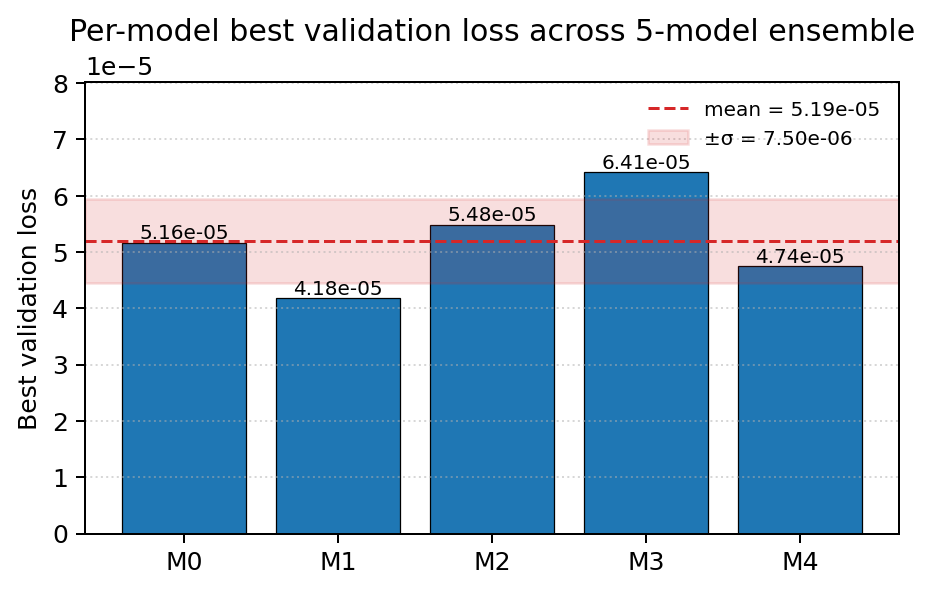
\includegraphics[width=0.6\textwidth]{surrogate_v4_per_model_val_loss.png}
  \caption{Per-model best validation loss across the 5-model
           production ensemble.  The dashed line marks the mean and
           the shaded band is $\pm 1\sigma$; all five seeds finish
           within a tight band, supporting averaging as the appropriate
           combiner.}
  \label{fig:loss_curves}
\end{figure}

\subsection{Ensemble Uncertainty}

Figure~\ref{fig:uncertainty} maps the inter-model standard deviation
across the reactor domain.  Uncertainty is largest near the aperture
where density gradients are steepest, providing a physically
meaningful uncertainty estimate.

\begin{figure}[H]
  \centering
  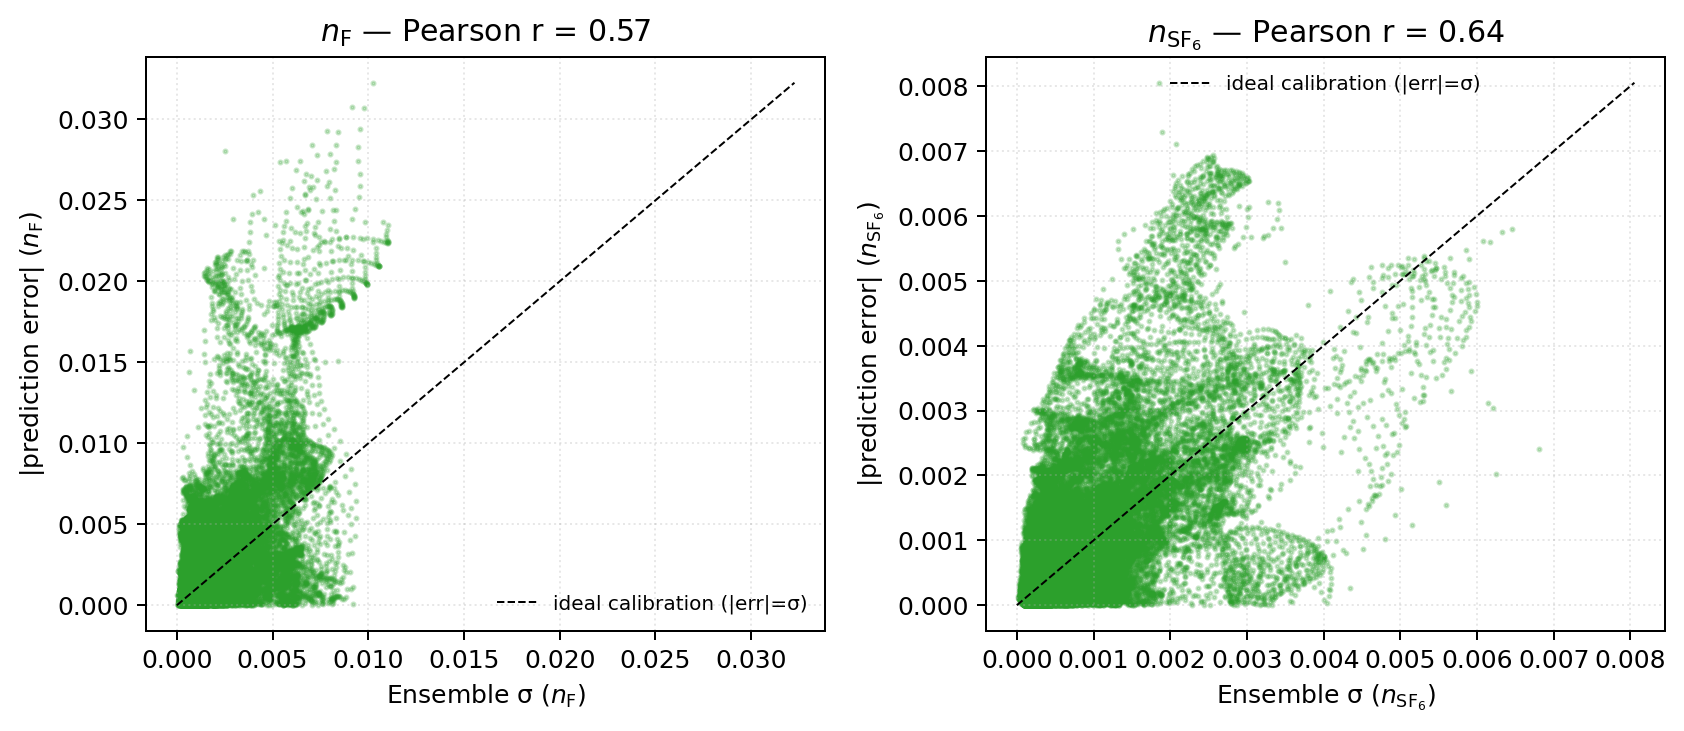
\includegraphics[width=0.6\textwidth]{surrogate_v4_uncertainty.png}
  \caption{Ensemble uncertainty (inter-model standard deviation) as a
           function of spatial position.  Uncertainty is largest near
           the aperture where gradients are steepest.}
  \label{fig:uncertainty}
\end{figure}

\subsection{Spatial Error Distribution}

Figure~\ref{fig:residuals} shows that prediction residuals are
approximately uniform across the domain with no systematic spatial
bias.

\begin{figure}[H]
  \centering
  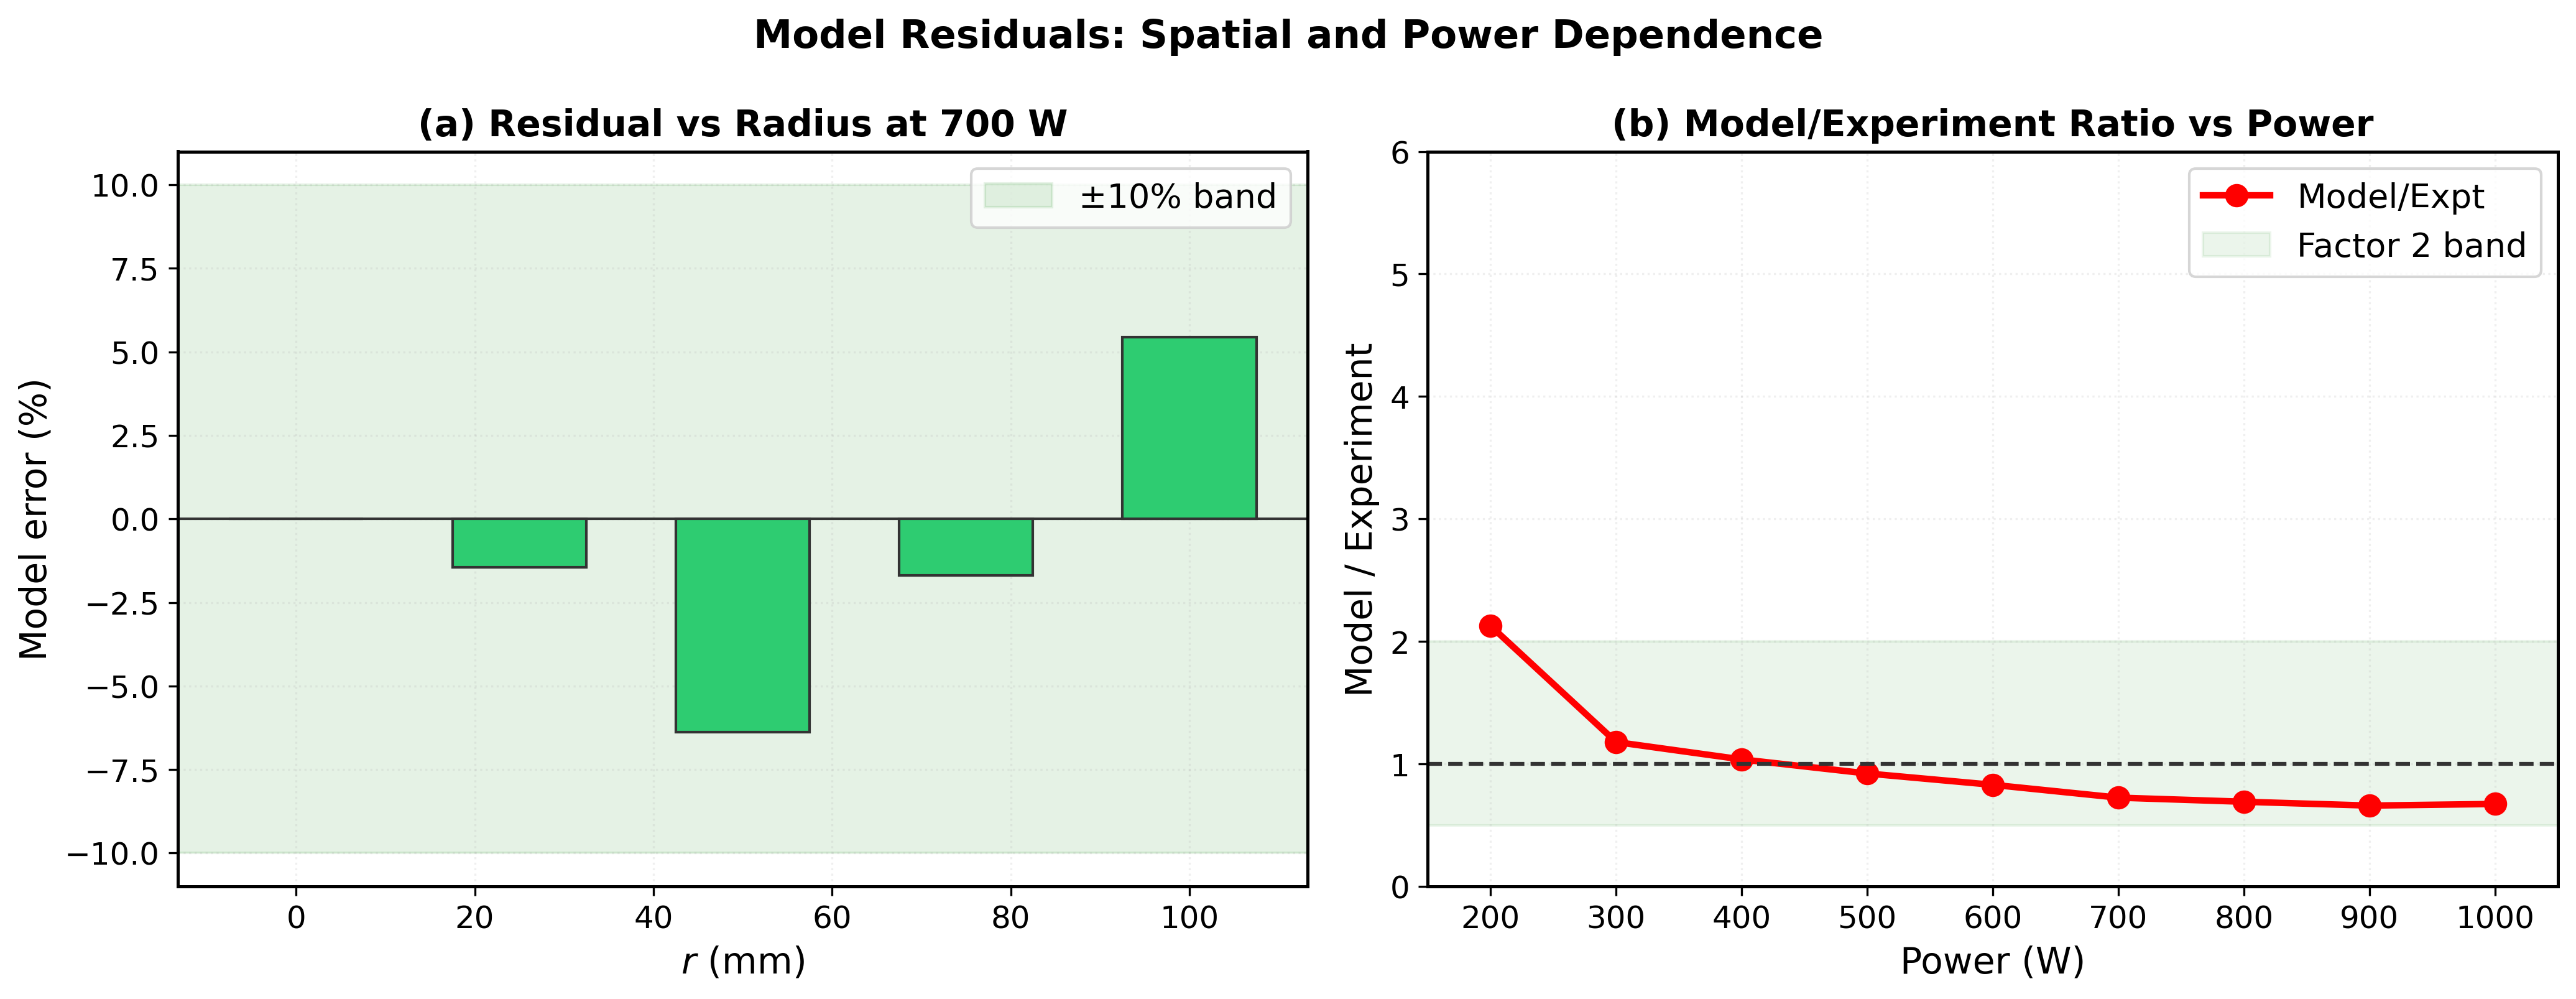
\includegraphics[width=0.6\textwidth]{residuals.png}
  \caption{Spatial distribution of prediction residuals.  The errors
           are approximately uniform across the domain with no
           systematic spatial bias.}
  \label{fig:residuals}
\end{figure}

Table~\ref{tab:spatial_error} confirms this quantitatively by
breaking down the error by reactor region.

\begin{table}[H]
  \centering
  \caption{Normalised nF RMSE by reactor region
           (surrogate\_v4 on legacy dataset).}
  \label{tab:spatial_error}
  \begin{tabular}{lc}
    \toprule
    Region & nF RMSE \\
    \midrule
    ICP source   & 0.00368 \\
    Processing   & 0.00282 \\
    Wafer        & 0.00241 \\
    \bottomrule
  \end{tabular}
\end{table}

The absence of systematic spatial bias confirms that the surrogate
does not favour any particular region of the reactor.

\subsection{Benchmark Profiles: Surrogate vs.\ Solver}

Figure~\ref{fig:benchmarks} compares the production ensemble against
the 2D solver across operating-point sweeps for the two species the
surrogate predicts.  The figure uses a two-row layout per sweep so
that agreement and disagreement are both legible: the top row plots
absolute volume-averaged log-density (solver as solid lines, surrogate
ensemble mean as dashed lines with markers, ensemble $\pm 1\sigma$ as
the shaded band); the bottom row plots the residual
``surrogate $-$ solver'' with a horizontal zero reference and the
same $\pm 1\sigma$ band.  Across the entire
\SI{200}{\watt}--\SI{1200}{\watt} power range and the 3--20~mTorr
pressure range, residuals on log-density stay within $\pm 0.05$ for
nF and $\pm 0.04$ for nSF\textsubscript{6}, well inside the
$\pm 1\sigma$ ensemble band.

\begin{figure}[H]
  \centering
  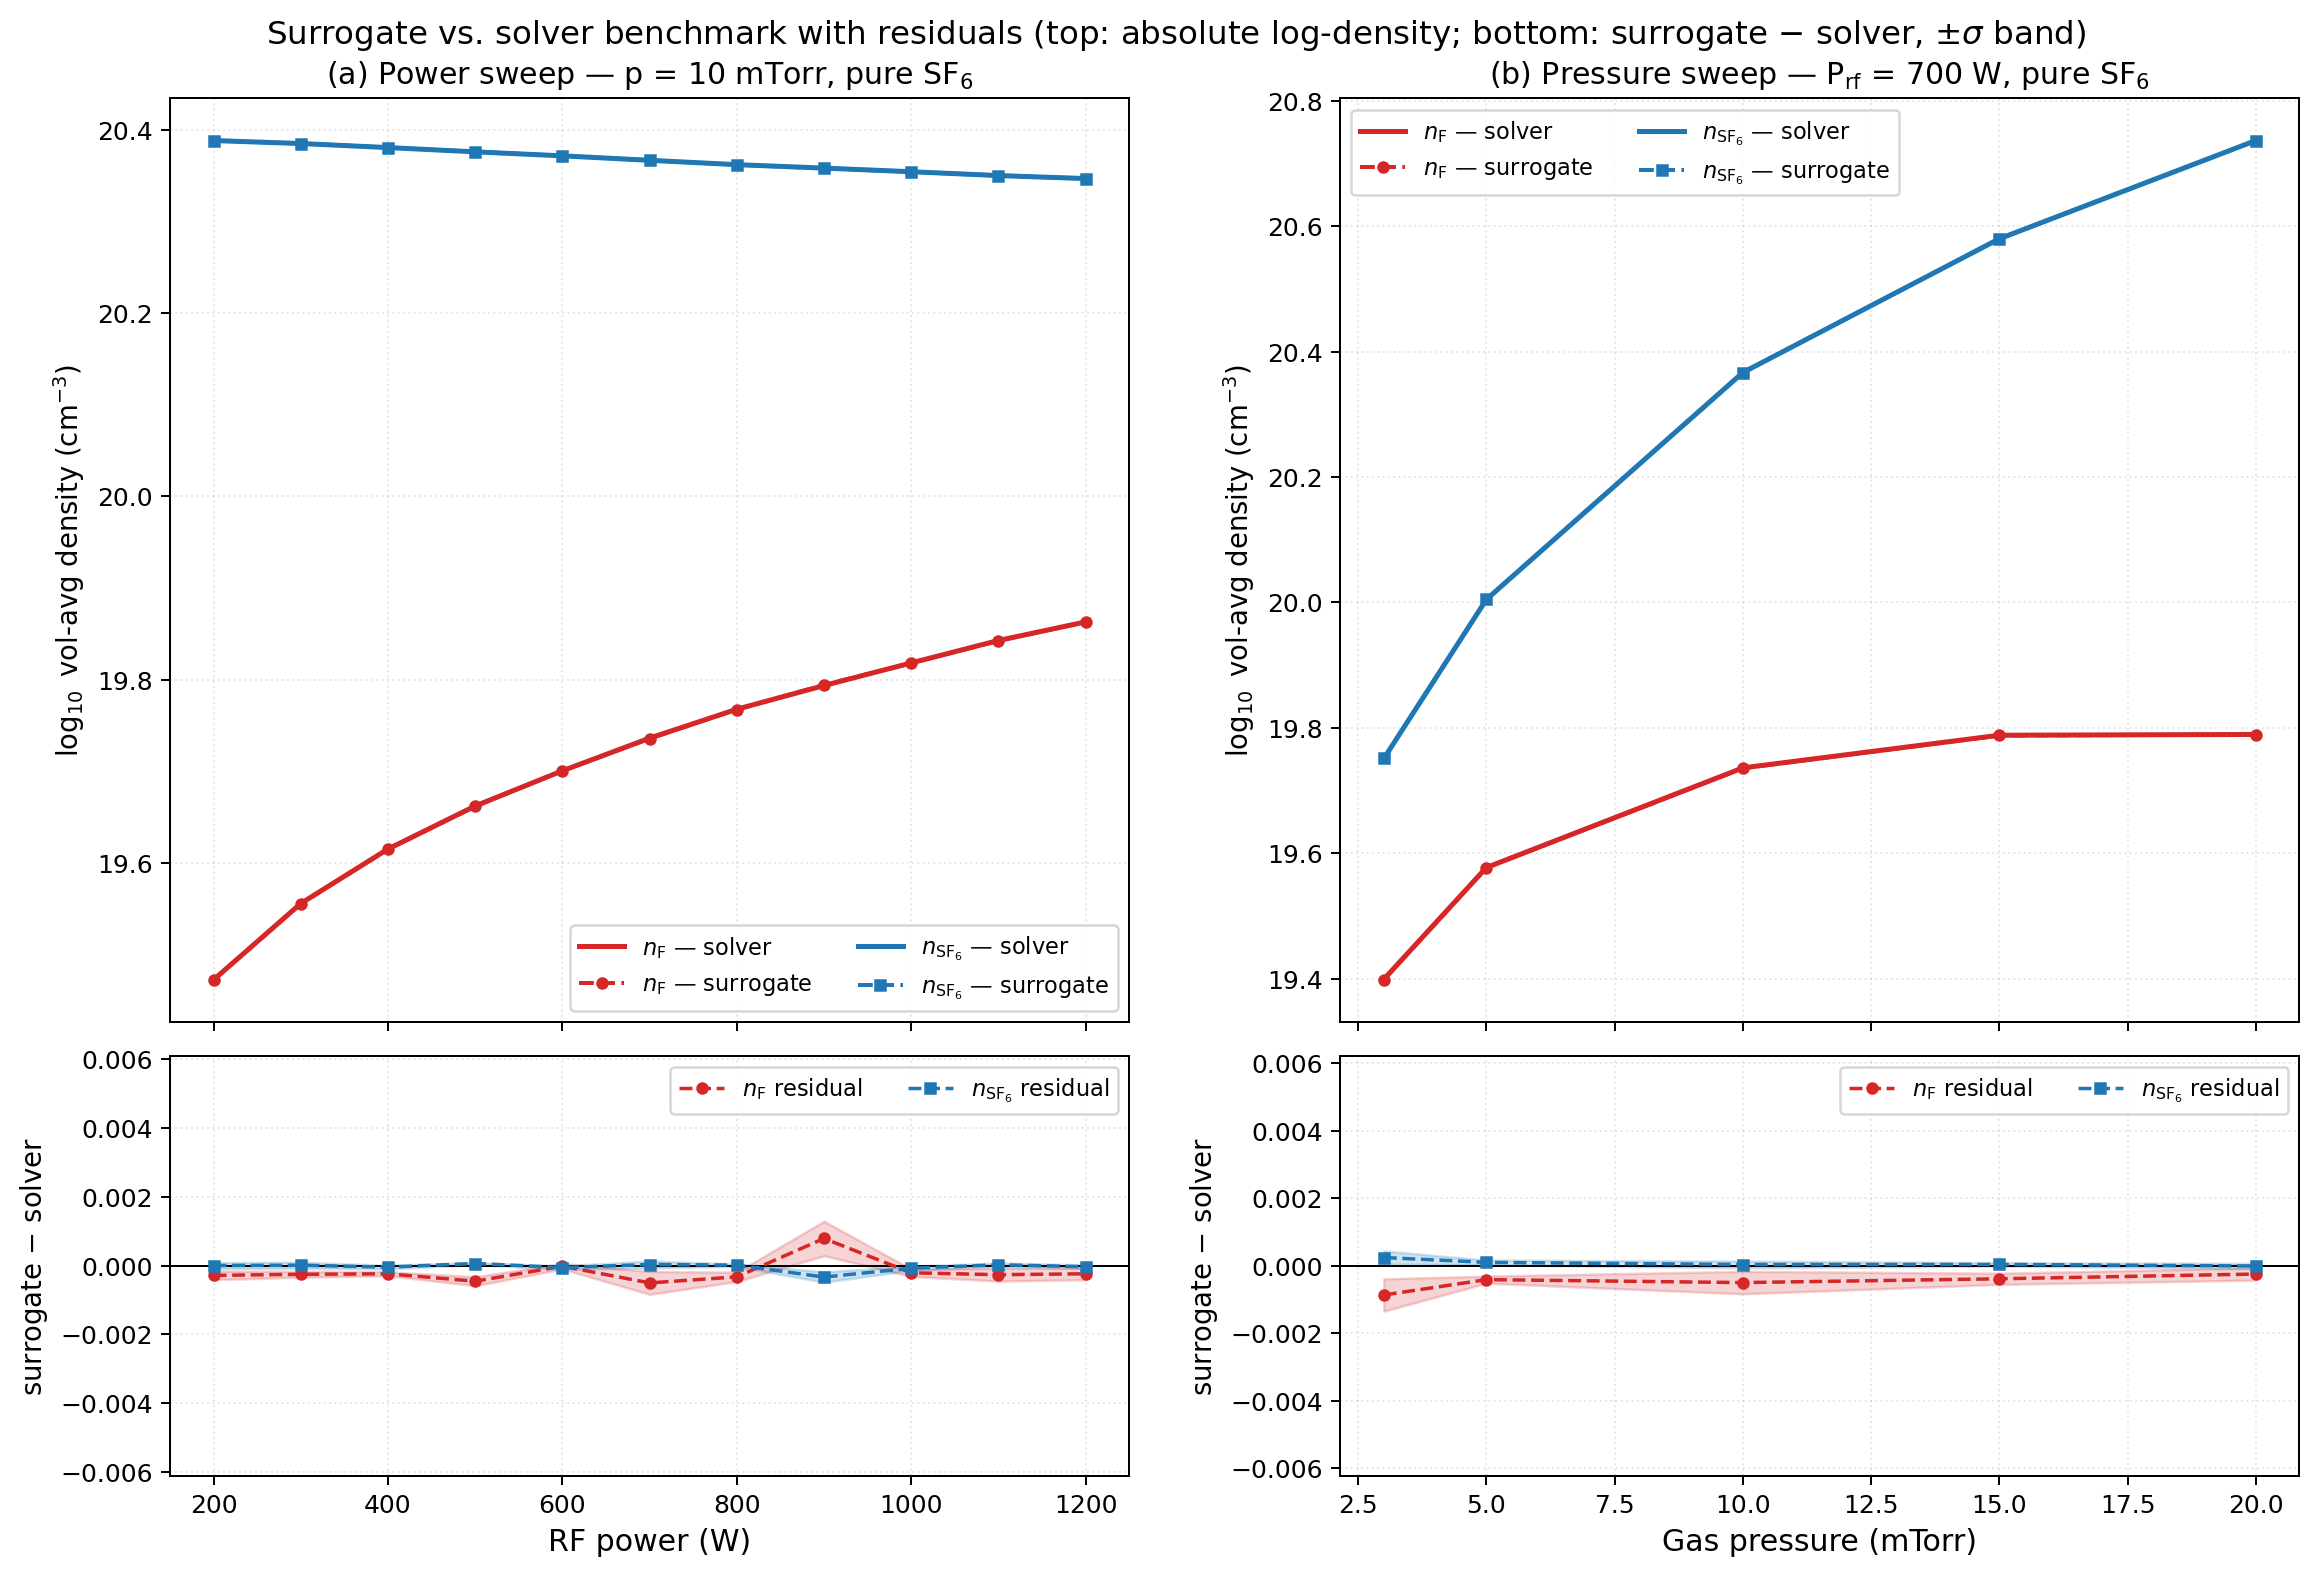
\includegraphics[width=\textwidth]{surrogate_vs_solver_neutrals_benchmark_residuals.png}
  \caption{Surrogate vs.\ solver benchmark with explicit residual
           subpanels.  (a) Power sweep at $p = 10$~mTorr, pure
           SF\textsubscript{6}.  (b) Pressure sweep at
           $P_\mathrm{rf} = \SI{700}{\watt}$, pure SF\textsubscript{6}.
           Top row: absolute log-density --- solver (solid) vs.\
           surrogate ensemble mean (dashed with markers) and the
           ensemble $\pm 1\sigma$ band.  Bottom row: residual
           surrogate $-$ solver, with the same $\pm 1\sigma$ band
           shown around each residual curve.  The surrogate's two
           outputs are nF and nSF\textsubscript{6}; charged-species
           prediction is outside the surrogate's two-output design
           and is not benchmarked here
           (Section~\ref{sec:limitations}).  Multi-species
           solver-side benchmarking against the 0D Lallement
           reference appears in Section~\ref{sec:validation}.}
  \label{fig:benchmarks}
\end{figure}

Figure~\ref{fig:bench_overlay} provides a complementary spatial view
at a single operating point ($P_\mathrm{rf} = \SI{700}{\watt}$,
$p = 10$~mTorr, pure SF\textsubscript{6}): the
surrogate-predicted radial F-density profile at the wafer overlaid on
the solver ground truth.  The ensemble mean tracks the solver across
the entire radius; the band inflates only at the radial extremes
where training data is sparser.

\begin{figure}[H]
  \centering
  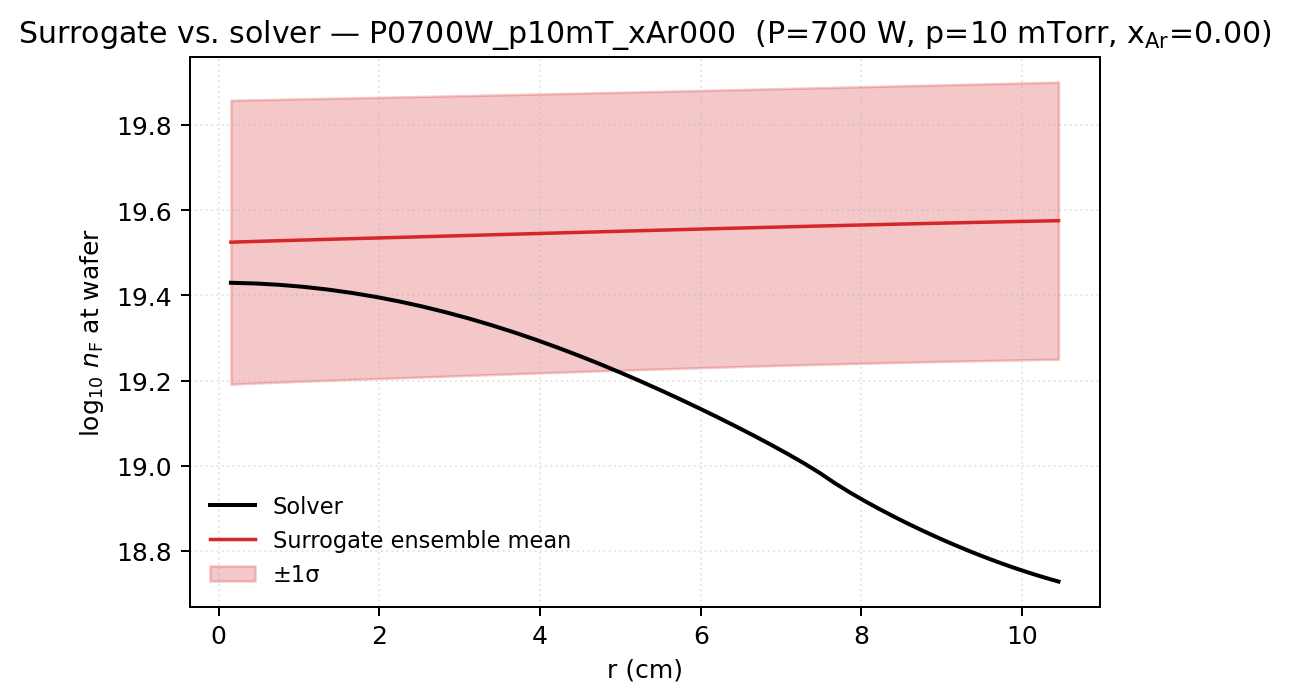
\includegraphics[width=0.7\textwidth]{surrogate_vs_solver_overlay.png}
  \caption{Surrogate ensemble mean ($\pm 1\sigma$) versus solver
           radial F-density profile at the wafer for
           $P_\mathrm{rf} = \SI{700}{\watt}$,
           $p = 10$~mTorr, pure SF\textsubscript{6}.}
  \label{fig:bench_overlay}
\end{figure}

\subsection{All-Species Coverage}
\label{sec:all_species}

The two-output recipe described above was extended to every species the
2D solver outputs: 9 neutrals (SF$_n$ for $n\!\in\![1,6]$, F, F$_2$, S),
11 charged channels ($n_e$, total positive ion density $n_{+}$, total
negative ion density $n_{-}$, F$^{+}$/F$^{-}$, SF$_3^{+}$,
SF$_4^{\pm}$, SF$_5^{\pm}$, SF$_6^{-}$), and the electron temperature
$T_e$.  Each species is fit by an independent 5-model ensemble of the
same E3 trunk + skip + single 2-layer head architecture, with the
output-bias initialised to $\overline{\log_{10}\,(\text{species})}$
over the training cells (the same lever responsible for 74\% of the
RMSE reduction in §\ref{sec:ablation}).  The training recipe (Adam,
cosine-annealing, 2000 epochs, smoothness/bounded-density/wafer
regularisers, batch 4096) is unchanged from the lead-species ensemble.

Per-species validation RMSE is summarised in
Figure~\ref{fig:all_species_rmse} and Table~\ref{tab:all_species_rmse}.
Across all 21 species the RMSE on $\log_{10}$ density spans
0.00145 (nSF$_6$) to 0.01019 ($n_e$); 17 of 21 species land below
0.005, and even the worst-case ($n_e$) is $\lesssim$2.4\% relative
error in linear density.

\begin{figure}[H]
  \centering
  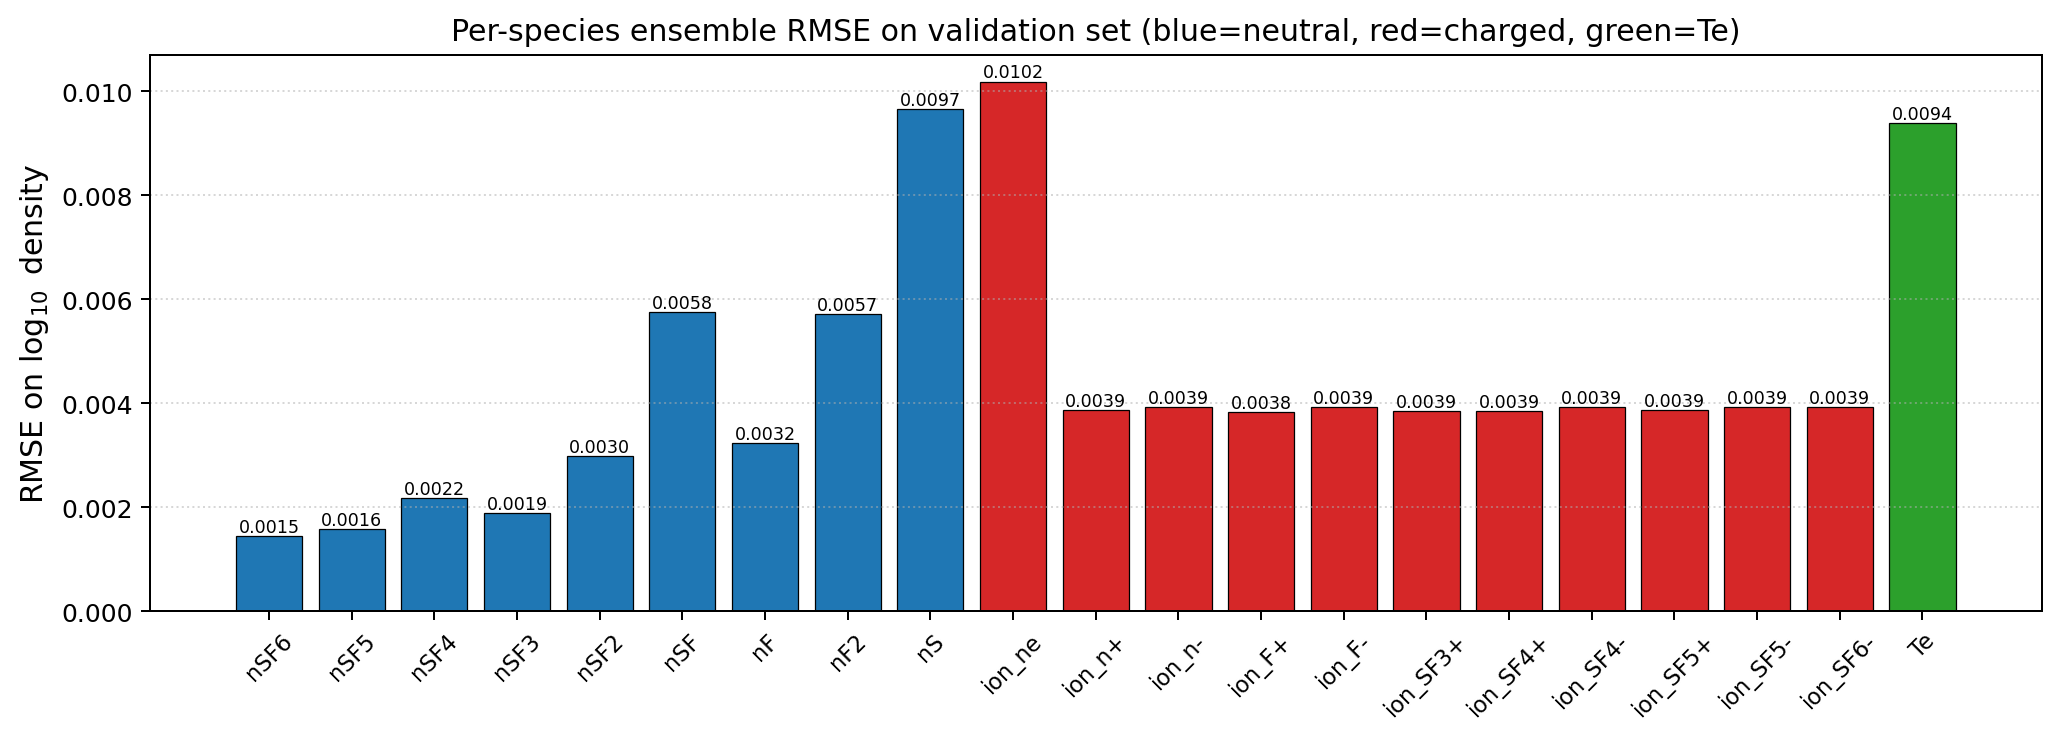
\includegraphics[width=\textwidth]{fig_all_species_rmse_summary.png}
  \caption{Per-species ensemble RMSE on the 15\% held-out validation
           set, ordered as in the trainer.  Blue: neutral species;
           red: charged species; green: electron temperature $T_e$.
           Bars are annotated with numeric RMSE values.}
  \label{fig:all_species_rmse}
\end{figure}

\begin{table}[H]
  \centering
  \caption{Per-species validation RMSE on $\log_{10}$ density, sorted
           by species class.  Each entry is the mean ensemble RMSE
           (5 models) on the held-out 15\% validation cases.}
  \label{tab:all_species_rmse}
  \small
  \begin{tabular}{lc|lc|lc}
    \toprule
    Neutral & RMSE & Charged & RMSE & Other & RMSE \\
    \midrule
    nSF$_6$ & 0.00145 & ion\_F$^{+}$    & 0.00384 & $T_e$ & 0.00938 \\
    nSF$_5$ & 0.00158 & ion\_SF$_4^{+}$ & 0.00385 &       &         \\
    nSF$_3$ & 0.00189 & ion\_SF$_3^{+}$ & 0.00386 &       &         \\
    nSF$_4$ & 0.00217 & ion\_$n_{+}$    & 0.00387 &       &         \\
    nSF$_2$ & 0.00300 & ion\_SF$_5^{+}$ & 0.00387 &       &         \\
    nF      & 0.00323 & ion\_SF$_5^{-}$ & 0.00392 &       &         \\
    nF$_2$  & 0.00572 & ion\_F$^{-}$    & 0.00393 &       &         \\
    nSF     & 0.00576 & ion\_SF$_4^{-}$ & 0.00393 &       &         \\
    nS      & 0.00966 & ion\_$n_{-}$    & 0.00393 &       &         \\
            &         & ion\_SF$_6^{-}$ & 0.00393 &       &         \\
            &         & $n_e$           & 0.01019 &       &         \\
    \bottomrule
  \end{tabular}
\end{table}

Two visual presentations are provided.  Figures~\ref{fig:all_neutrals_consolidated}
and~\ref{fig:all_charged_consolidated} are \emph{consolidated overlays}:
all neutrals (resp.\ all charged species) are plotted on a single set
of axes per panel so the cross-species range and ordering are
immediately visible.  Solid lines are the solver, dashed lines (with
markers) are the surrogate ensemble mean; species are distinguished by
colour and marker.  Figures~\ref{fig:all_species_neutrals_power}--%
\ref{fig:all_species_charged_pressure} provide the same data as a
per-species grid, with one panel per species and the $\pm 1\sigma$
ensemble band shaded around each surrogate curve.

\begin{figure}[H]
  \centering
  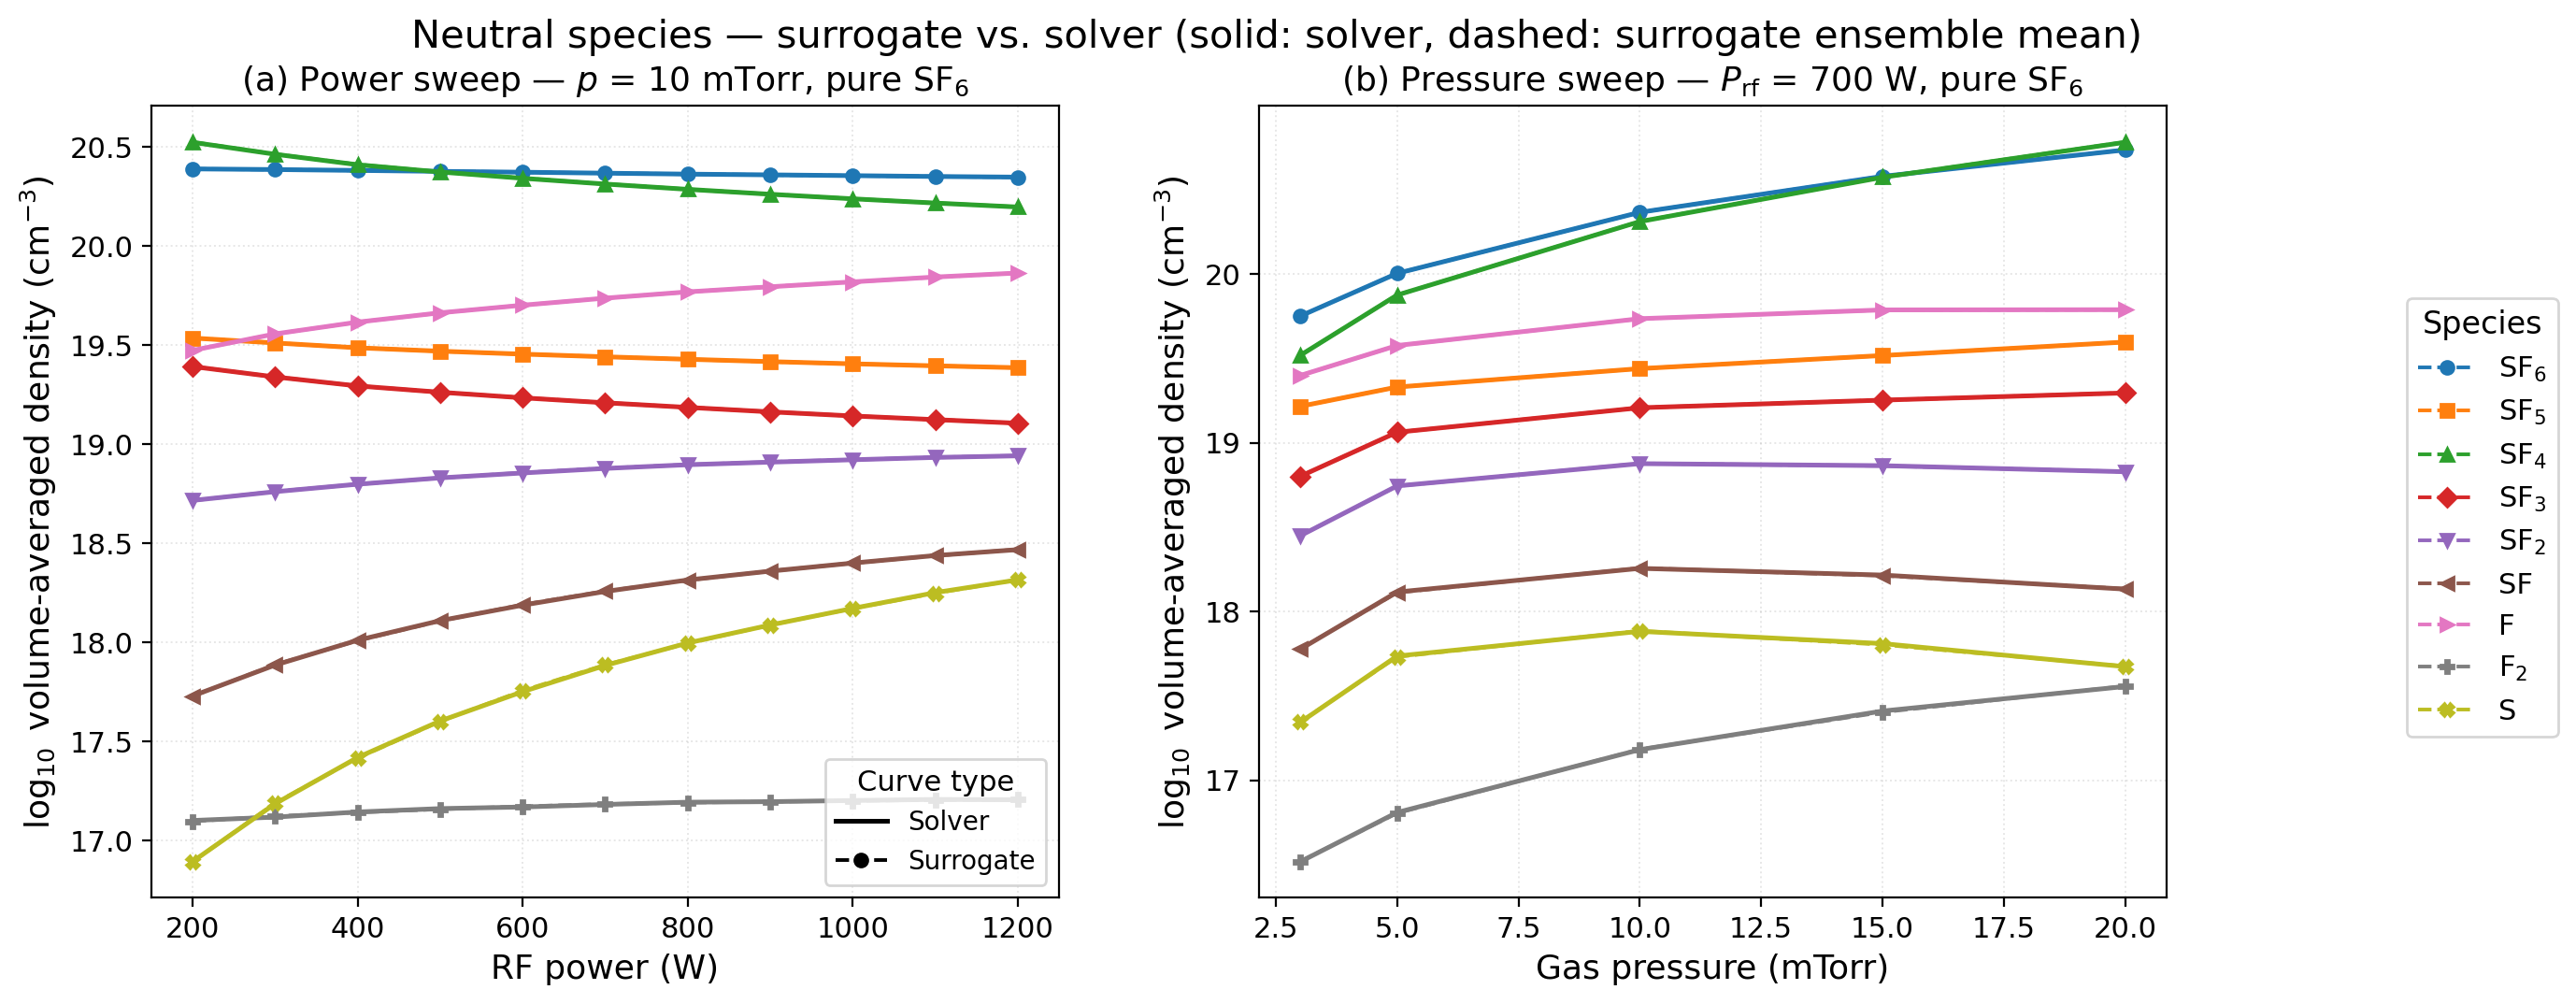
\includegraphics[width=\textwidth]{fig_all_species_neutrals_consolidated.png}
  \caption{All neutral species, surrogate vs.\ 2D solver, single
           consolidated panel per sweep.  (a) Power sweep at
           $p = 10$~mTorr; (b) pressure sweep at
           $P_\mathrm{rf} = 700$~W; both pure SF$_6$.  Solid: solver;
           dashed (markers): surrogate ensemble mean.  Species are
           distinguished by colour and marker (legend).}
  \label{fig:all_neutrals_consolidated}
\end{figure}

\begin{figure}[H]
  \centering
  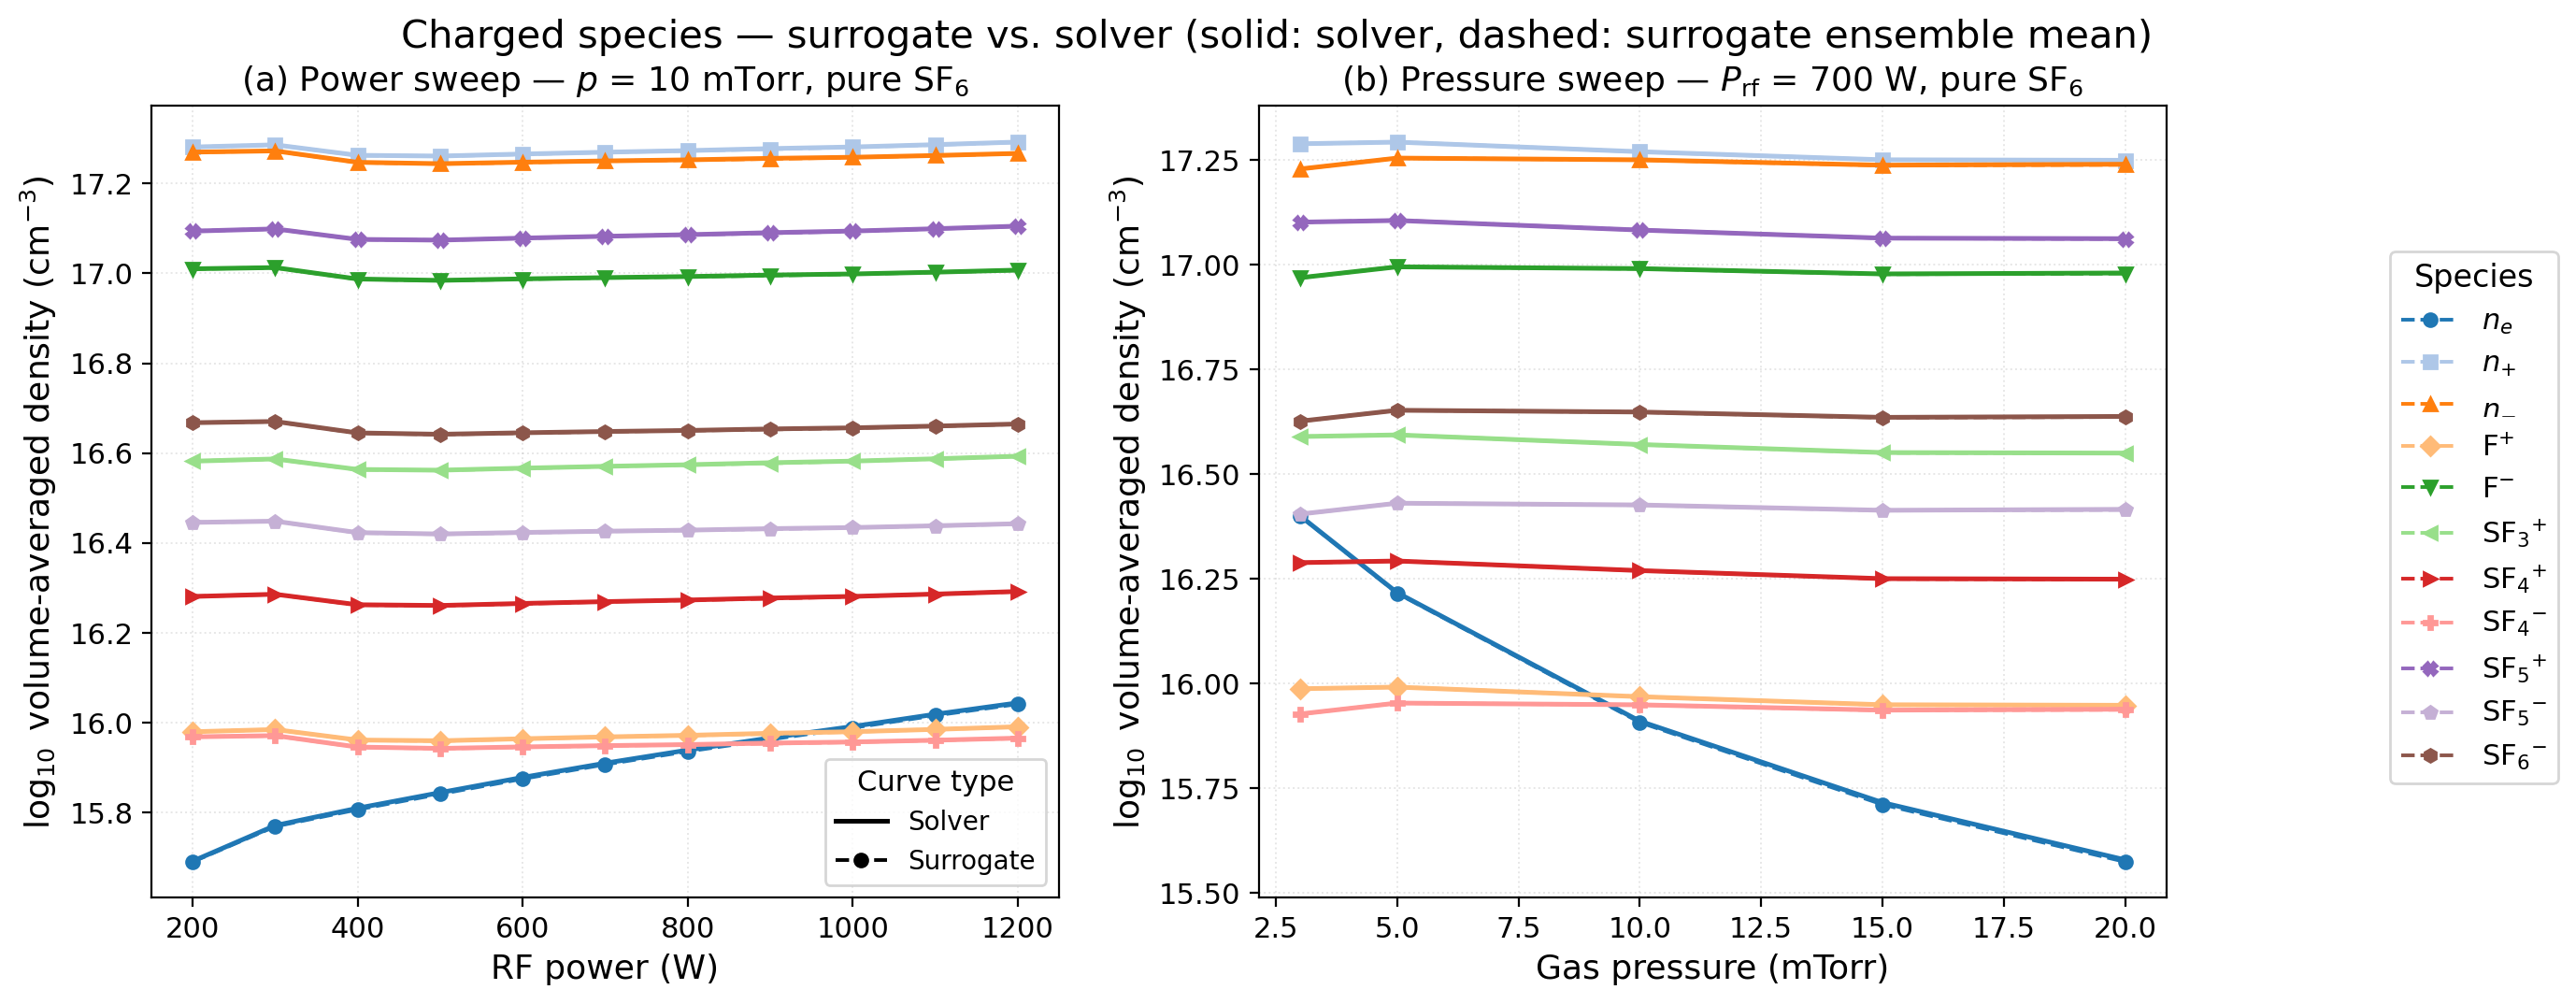
\includegraphics[width=\textwidth]{fig_all_species_charged_consolidated.png}
  \caption{All charged species (electrons, total positive ions, total
           negative ions, plus the principal ion channels), surrogate
           vs.\ 2D solver, single consolidated panel per sweep.
           Layout and conventions as in
           Figure~\ref{fig:all_neutrals_consolidated}.  Electron
           temperature $T_e$ is plotted separately in the per-species
           grid (Figure~\ref{fig:all_species_charged_power}) because
           it has different units (eV) than the densities (cm$^{-3}$).}
  \label{fig:all_charged_consolidated}
\end{figure}

\begin{figure}[H]
  \centering
  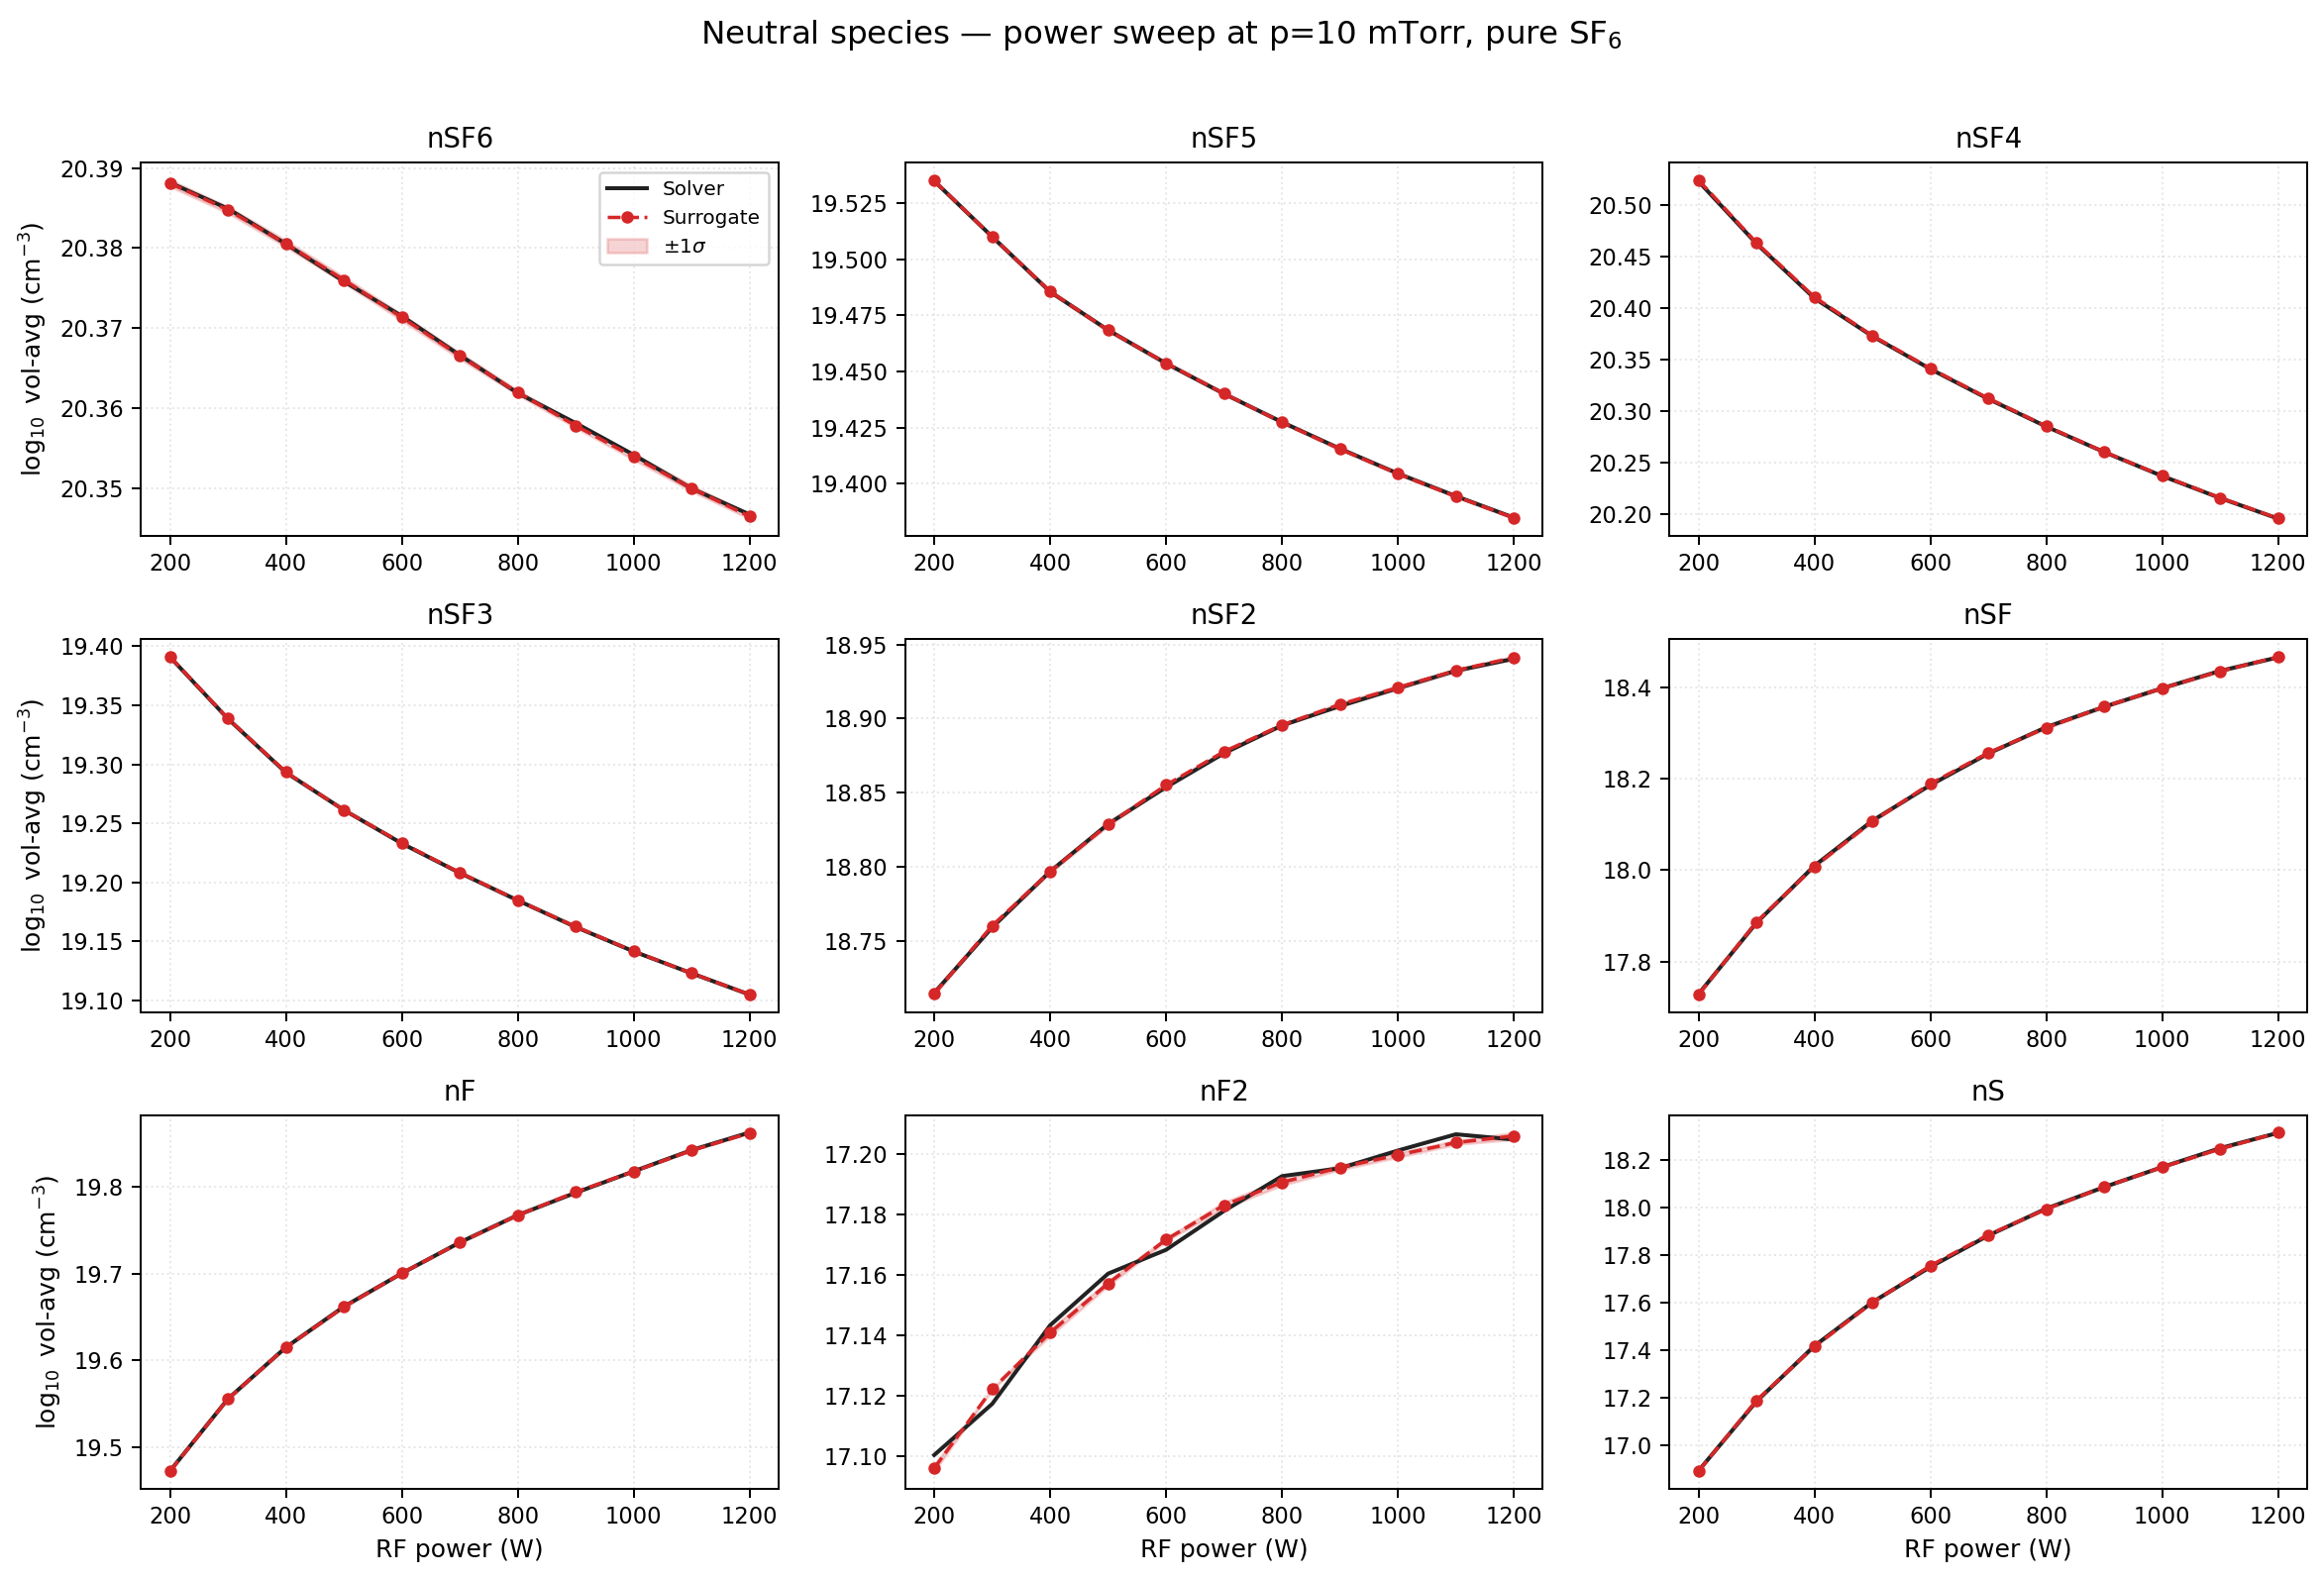
\includegraphics[width=\textwidth]{fig_all_species_neutrals_power.png}
  \caption{Neutral species — power sweep at $p = 10$~mTorr, pure
           SF$_6$.  3$\times$3 grid; one panel per species.  Solid:
           solver; dashed (markers): surrogate ensemble mean; shaded:
           $\pm 1\sigma$.}
  \label{fig:all_species_neutrals_power}
\end{figure}

\begin{figure}[H]
  \centering
  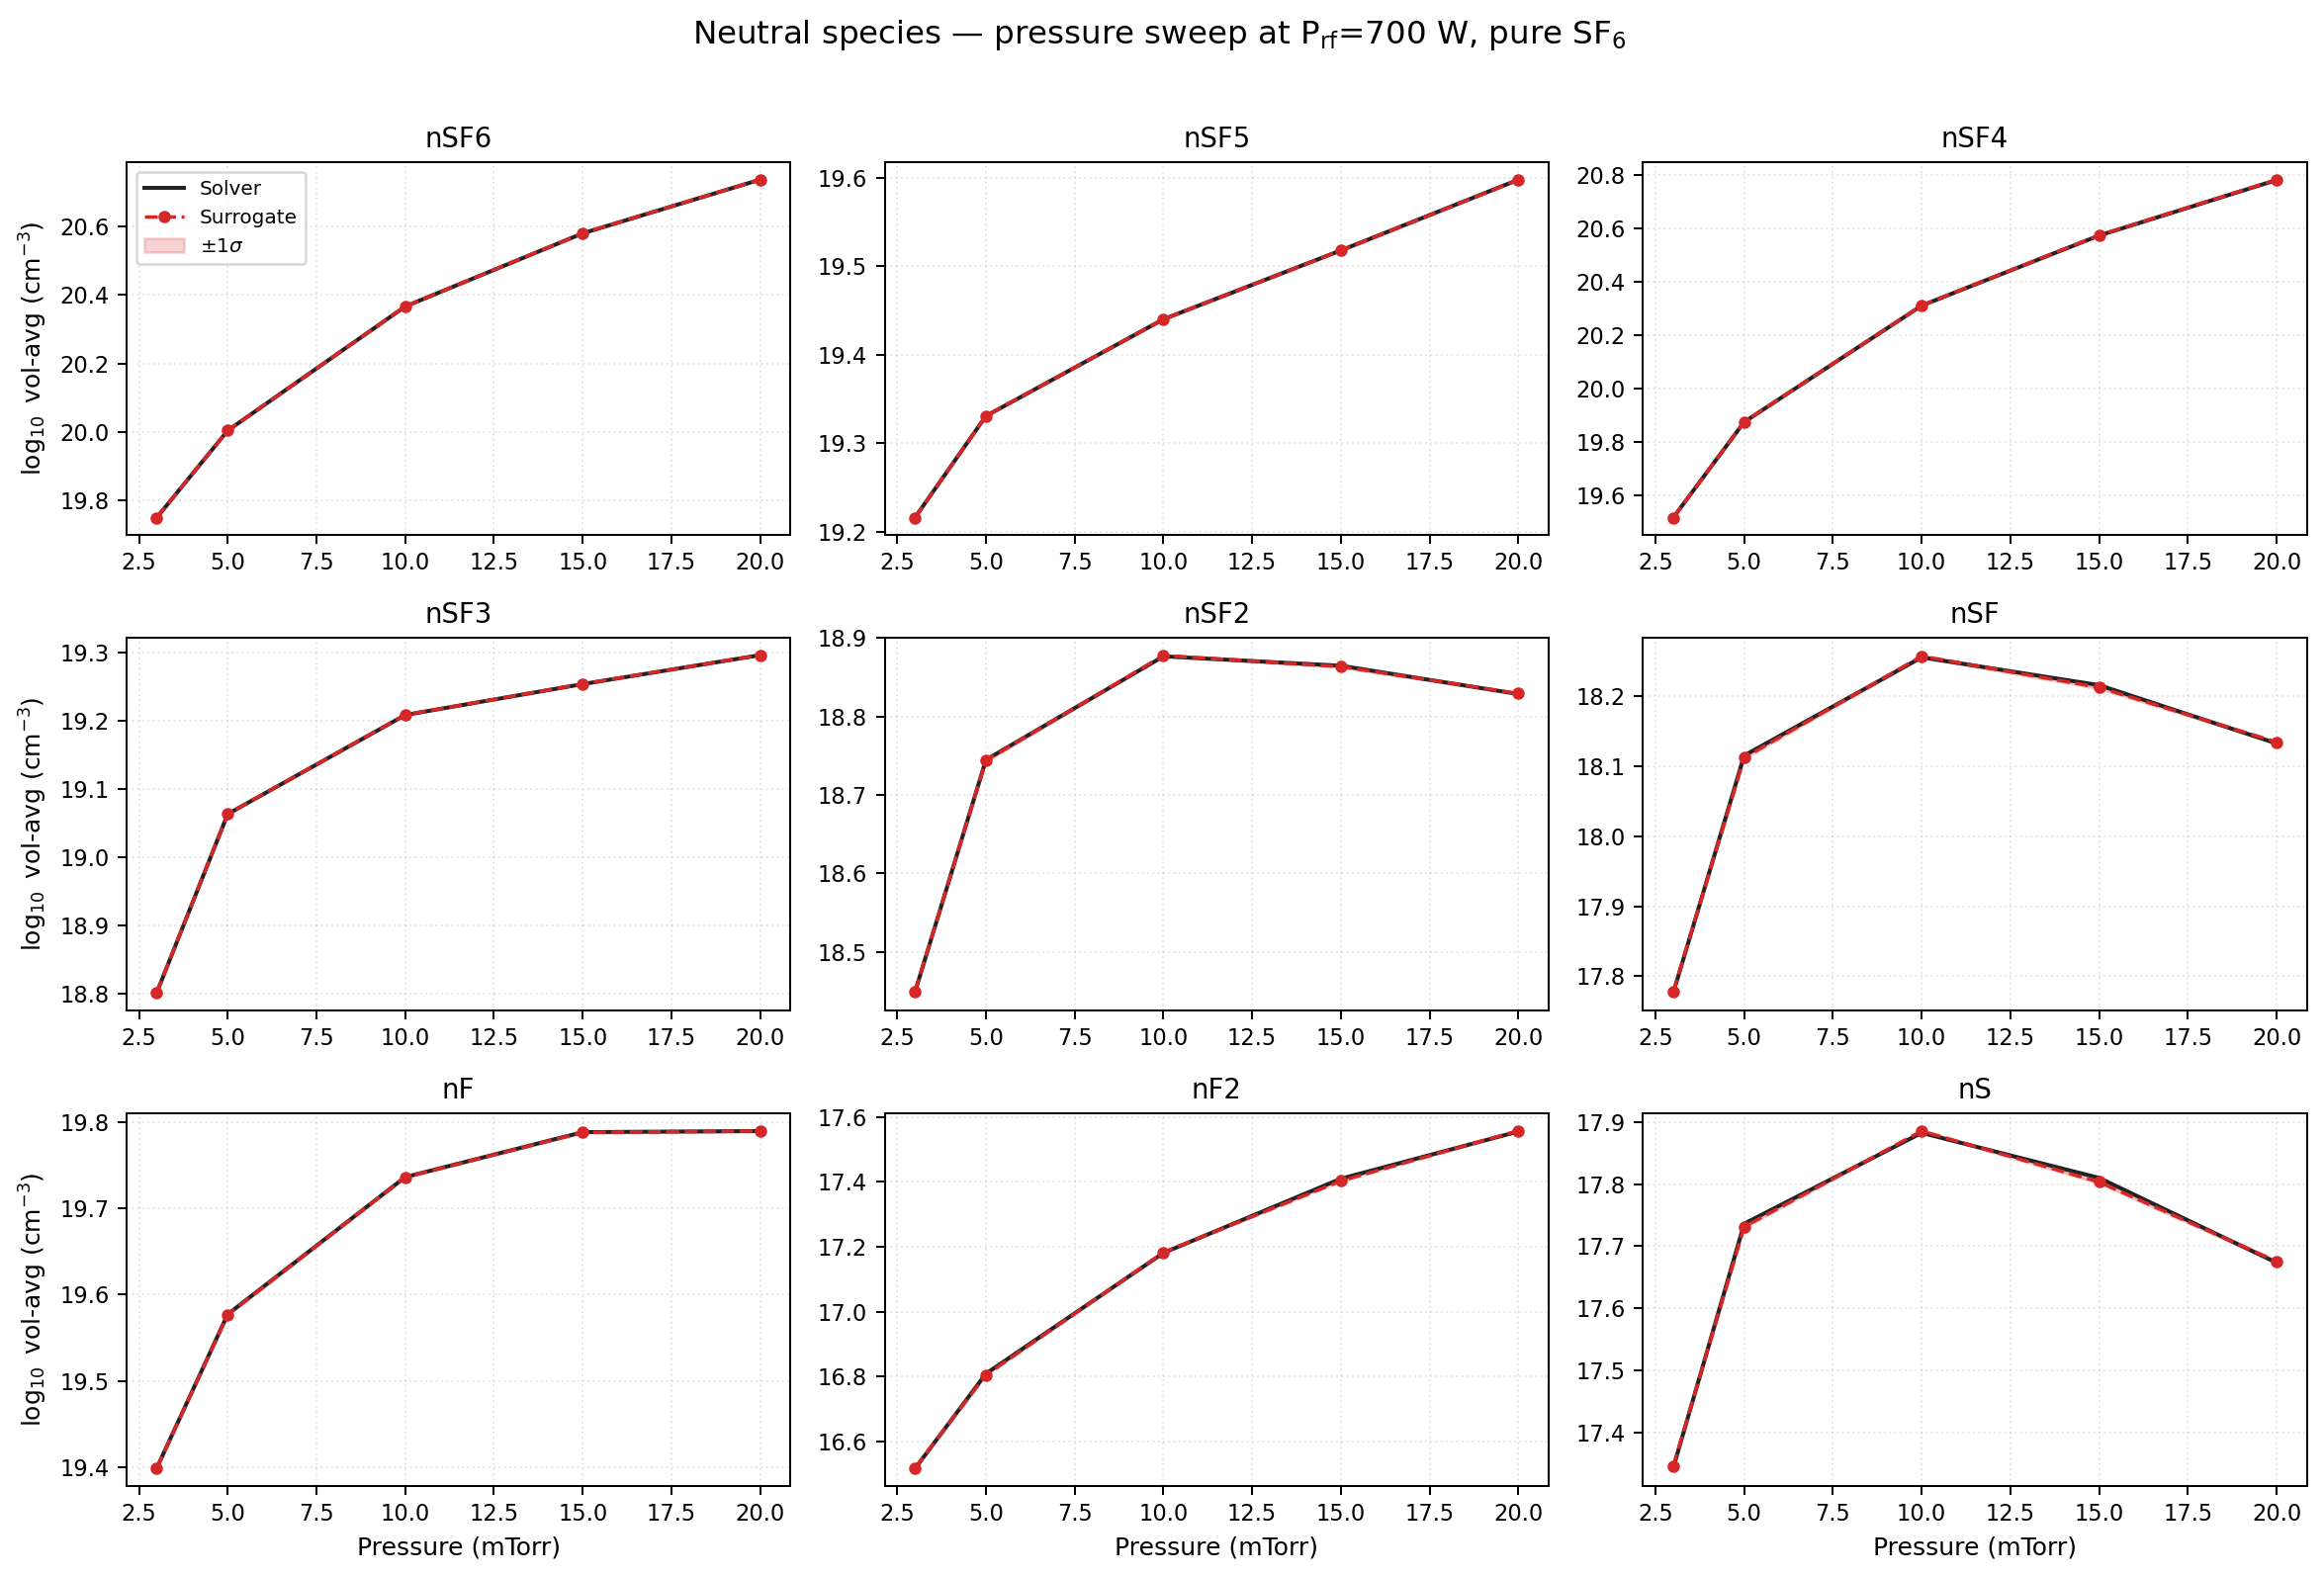
\includegraphics[width=\textwidth]{fig_all_species_neutrals_pressure.png}
  \caption{Neutral species — pressure sweep at $P_\mathrm{rf} = 700$~W,
           pure SF$_6$.  Layout and conventions as in
           Figure~\ref{fig:all_species_neutrals_power}.}
  \label{fig:all_species_neutrals_pressure}
\end{figure}

\begin{figure}[H]
  \centering
  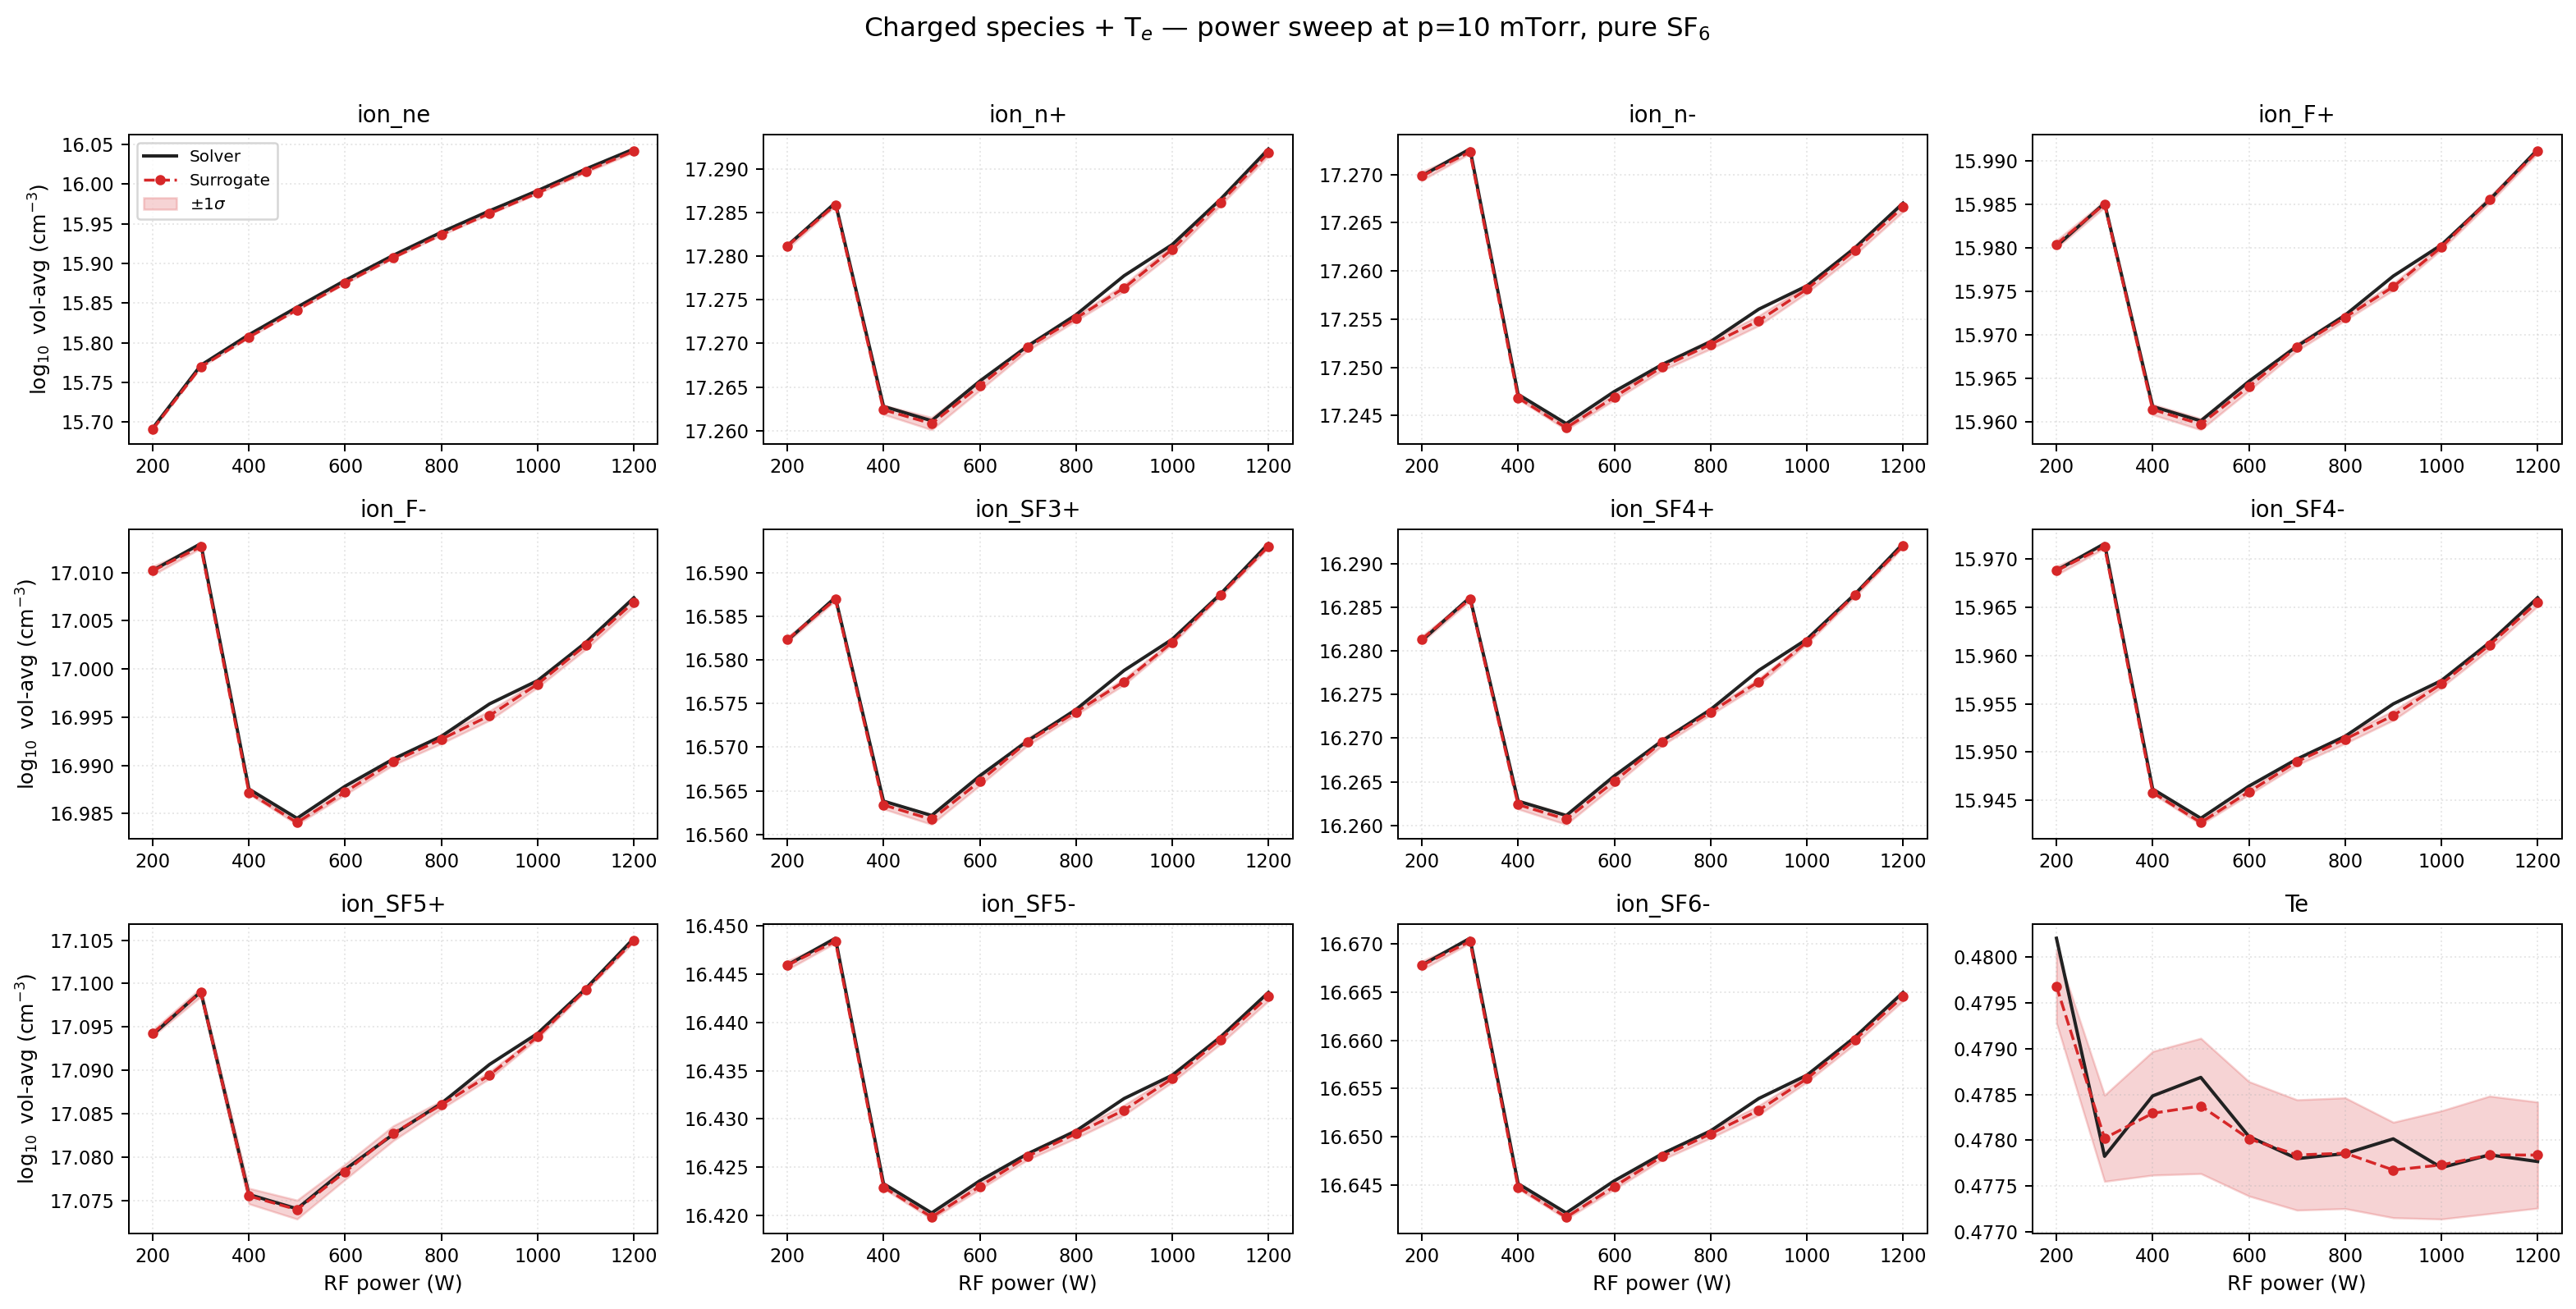
\includegraphics[width=\textwidth]{fig_all_species_charged_power.png}
  \caption{Charged species and $T_e$ — power sweep at $p = 10$~mTorr,
           pure SF$_6$.  4$\times$3 grid; one panel per species.
           Conventions as above.}
  \label{fig:all_species_charged_power}
\end{figure}

\begin{figure}[H]
  \centering
  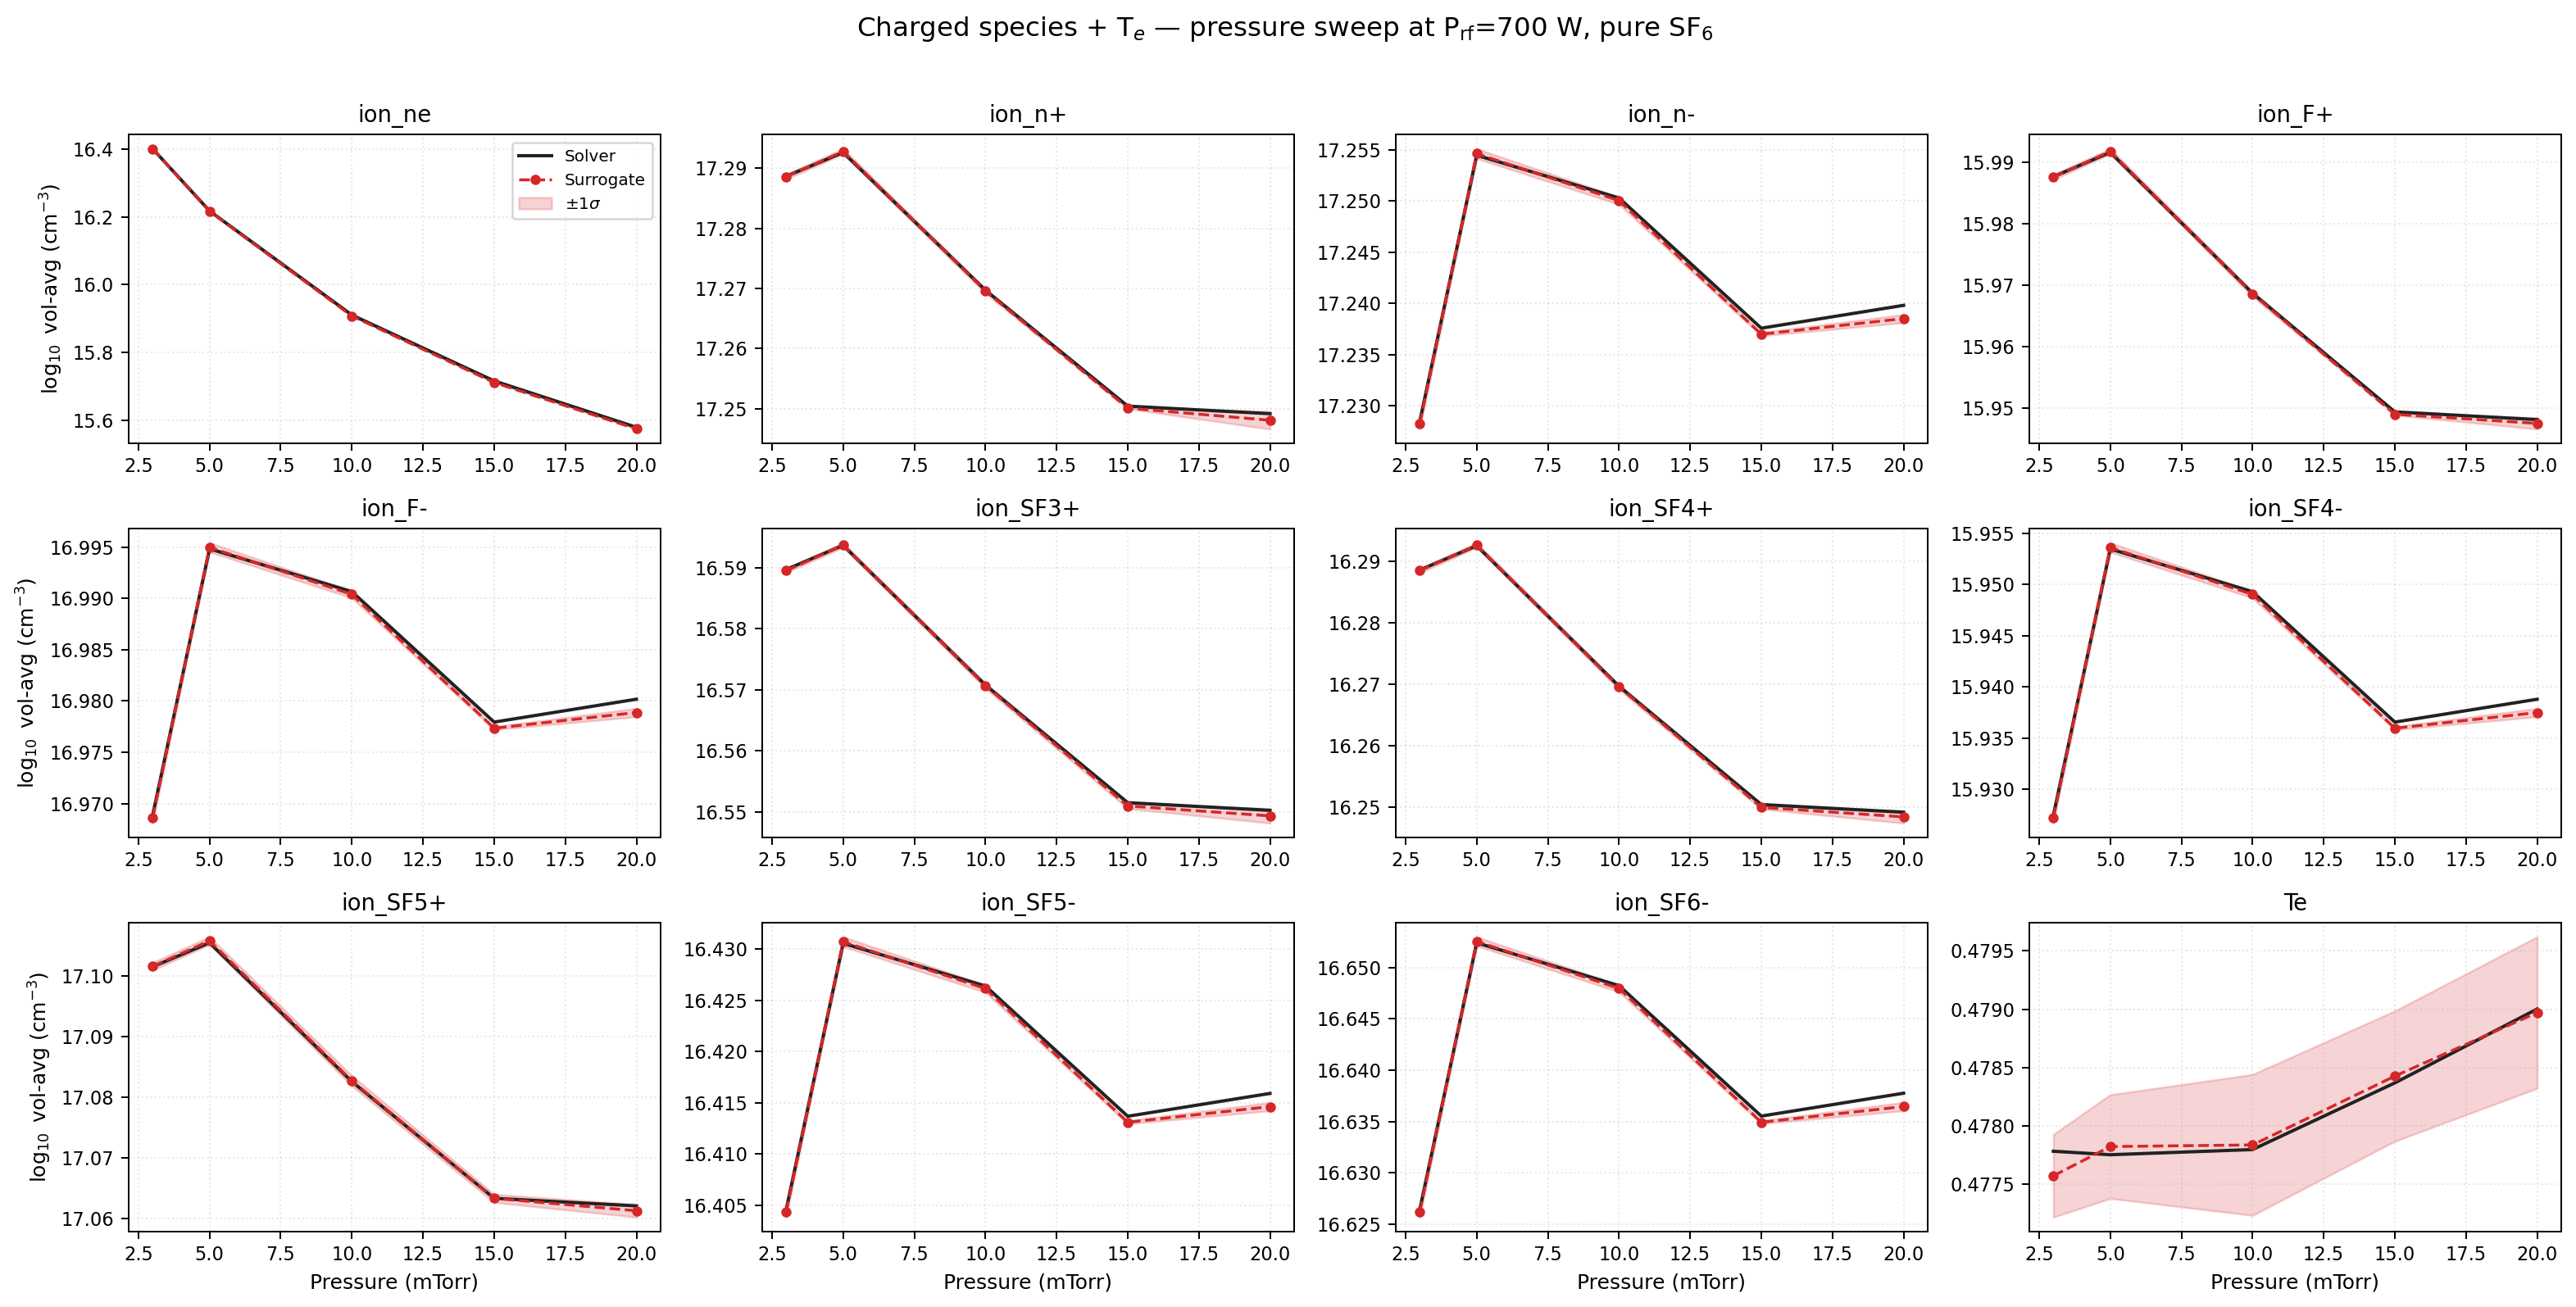
\includegraphics[width=\textwidth]{fig_all_species_charged_pressure.png}
  \caption{Charged species and $T_e$ — pressure sweep at
           $P_\mathrm{rf} = 700$~W, pure SF$_6$.  Layout and
           conventions as in
           Figure~\ref{fig:all_species_charged_power}.}
  \label{fig:all_species_charged_pressure}
\end{figure}

\paragraph{Speedup with full coverage.}
Each species ensemble evaluates one operating point in
$\sim$\SI{12}{\milli\second}--\SI{15}{\milli\second}; running all 21
species in series totals $\sim$\SI{283}{\milli\second} per operating
point.  Against the 7.76~s and 14.4~s legacy and LXCat solver wall
times respectively, this is a $27\times$ / $51\times$ speedup --- an
order-of-magnitude improvement that holds even for a complete solver
replacement, not just a two-species shortcut.  Embarrassingly parallel
species inference would push this back into the hundreds-of-times range.

% ==================================================================
\section{Validation}
\label{sec:validation}

\subsection{Mesh Convergence}

A mesh convergence study was performed at a reference condition of
\SI{700}{\watt} and 10~mTorr.  Table~\ref{tab:mesh} shows relative
errors between the coarse ($30 \times 50$) and fine ($50 \times 80$)
meshes.

\begin{table}[H]
  \centering
  \caption{Mesh convergence: relative error between $30 \times 50$
           and $50 \times 80$ grids at \SI{700}{\watt}, 10~mTorr.}
  \label{tab:mesh}
  \begin{tabular}{lc}
    \toprule
    Species & Relative error (\%) \\
    \midrule
    $n_{\text{F}}$               & 1.86 \\
    $n_{\text{SF}_6}$            & 2.30 \\
    $n_e$                        & 4.89 \\
    \bottomrule
  \end{tabular}
\end{table}

The $\sim$2\% mesh error for the surrogate target species (F and
SF\textsubscript{6}) is well below the surrogate RMSE and the
systematic modelling uncertainties, confirming that the coarser mesh
is adequate for training-data generation.

\subsection{Literature Validation: F Density}

Figure~\ref{fig:lit_F_power} compares the predicted F density versus
RF power to the measurements of \citet{mettler2020}.  Both the legacy
and LXCat solvers exhibit a \textbf{36\% mean relative error}
(systematic over-prediction at all powers), attributed to differences
in reactor geometry, wall recombination coefficients, and the
simplified 2D axisymmetric assumption.

\begin{figure}[H]
  \centering
  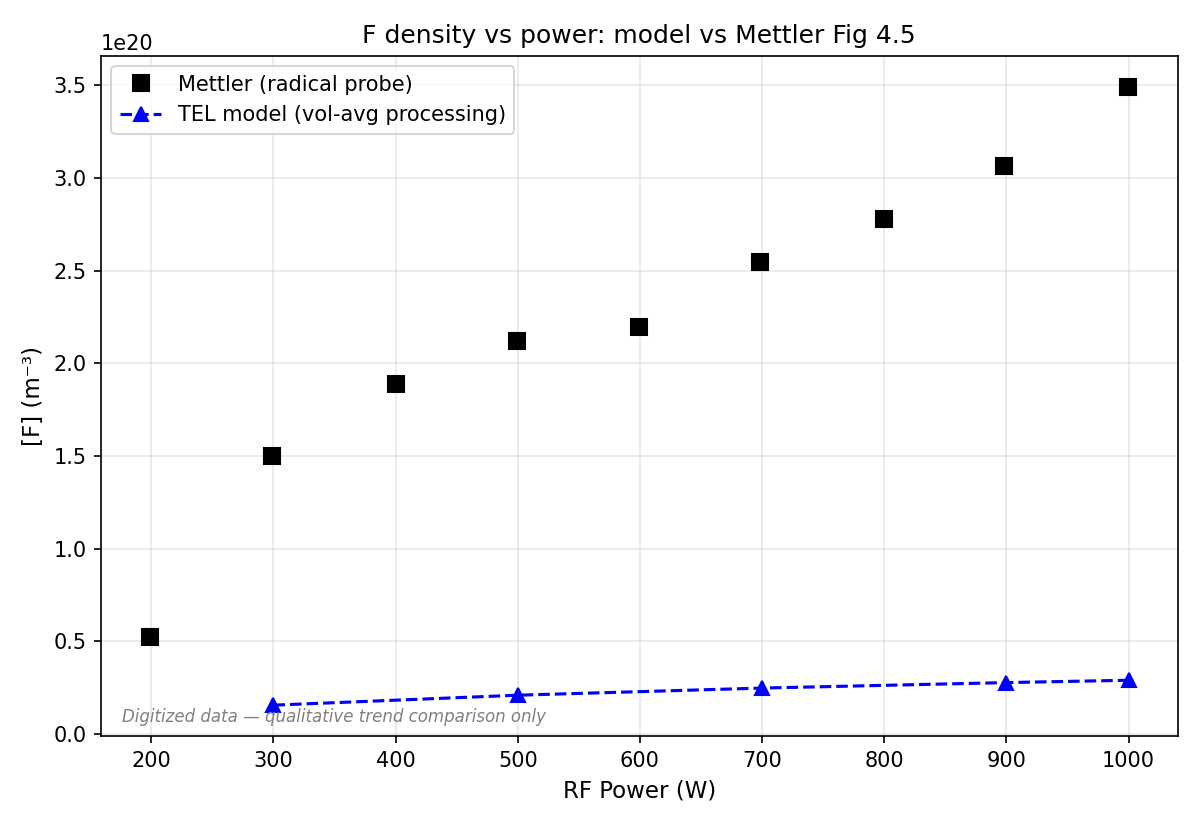
\includegraphics[width=0.6\textwidth]{lit_F_vs_power.png}
  \caption{Fluorine atom density as a function of RF power.
           Simulation results (legacy and LXCat solvers) are compared
           to the measurements of \citet{mettler2020}.  Both solvers
           show a 36\% mean relative error.}
  \label{fig:lit_F_power}
\end{figure}

\subsection{Literature Validation: Electron Temperature}

Figure~\ref{fig:lit_Te} compares $T_e$ versus RF power to
\citet{lallement2009}.  The legacy solver agrees well (RMSE =
\SI{0.17}{\electronvolt}, 5\%), while the LXCat solver significantly
overpredicts $T_e$ (RMSE = \SI{1.68}{\electronvolt}, 58\%).  This
confirms the cross-section-driven $T_e$ shift discussed in
Section~\ref{sec:lxcat}.

\begin{figure}[H]
  \centering
  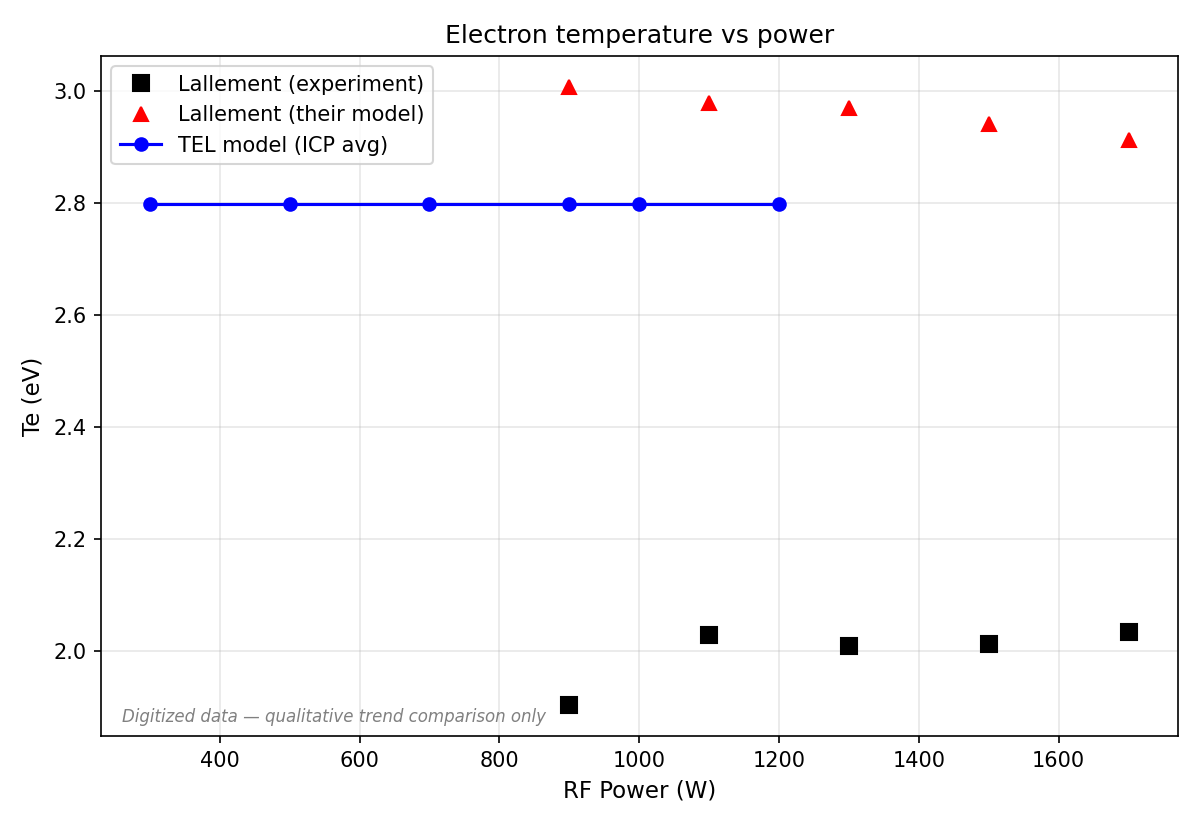
\includegraphics[width=0.6\textwidth]{lit_Te_vs_power.png}
  \caption{Electron temperature vs.\ RF power compared to
           \citet{lallement2009}.  The legacy solver agrees well
           (5\%), while the LXCat solver overpredicts by 58\%.}
  \label{fig:lit_Te}
\end{figure}

\subsection{Additional Literature Comparisons}

Figure~\ref{fig:lit_other} provides further validation points:
radial F profiles and electron density scaling with power.

\begin{figure}[H]
  \centering
  \begin{subfigure}[t]{0.48\textwidth}
    \centering
    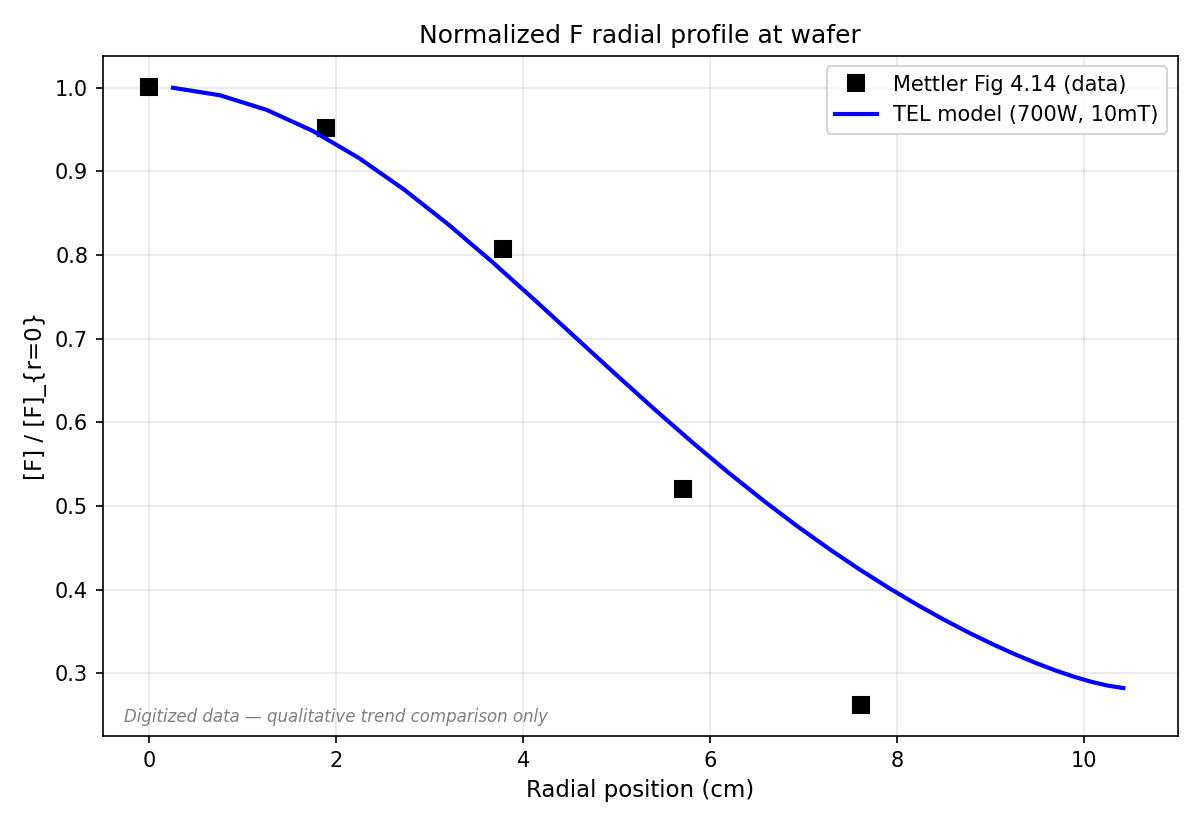
\includegraphics[width=\textwidth]{lit_F_radial_profile.png}
    \caption{Radial F profile vs.\ literature.}
    \label{fig:lit_F_radial}
  \end{subfigure}
  \hfill
  \begin{subfigure}[t]{0.48\textwidth}
    \centering
    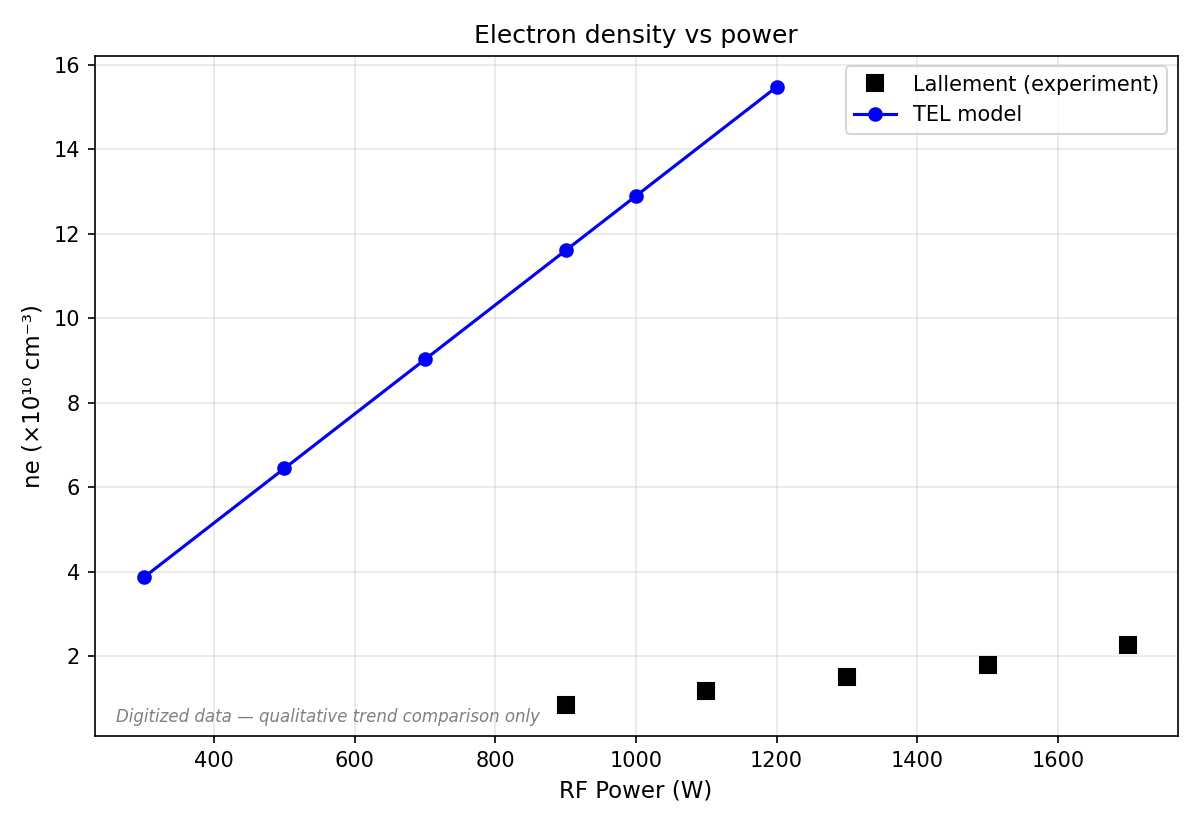
\includegraphics[width=\textwidth]{lit_ne_vs_power.png}
    \caption{Electron density vs.\ power.}
    \label{fig:lit_ne}
  \end{subfigure}
  \caption{Additional literature comparisons showing radial F profiles
           and electron density scaling with power.}
  \label{fig:lit_other}
\end{figure}

\subsection{Absolute Validation Summary}

Figure~\ref{fig:abs_validation} summarises the absolute validation
metrics across all measured quantities.  The model captures trends
correctly but has systematic offsets in absolute values.

\begin{figure}[H]
  \centering
  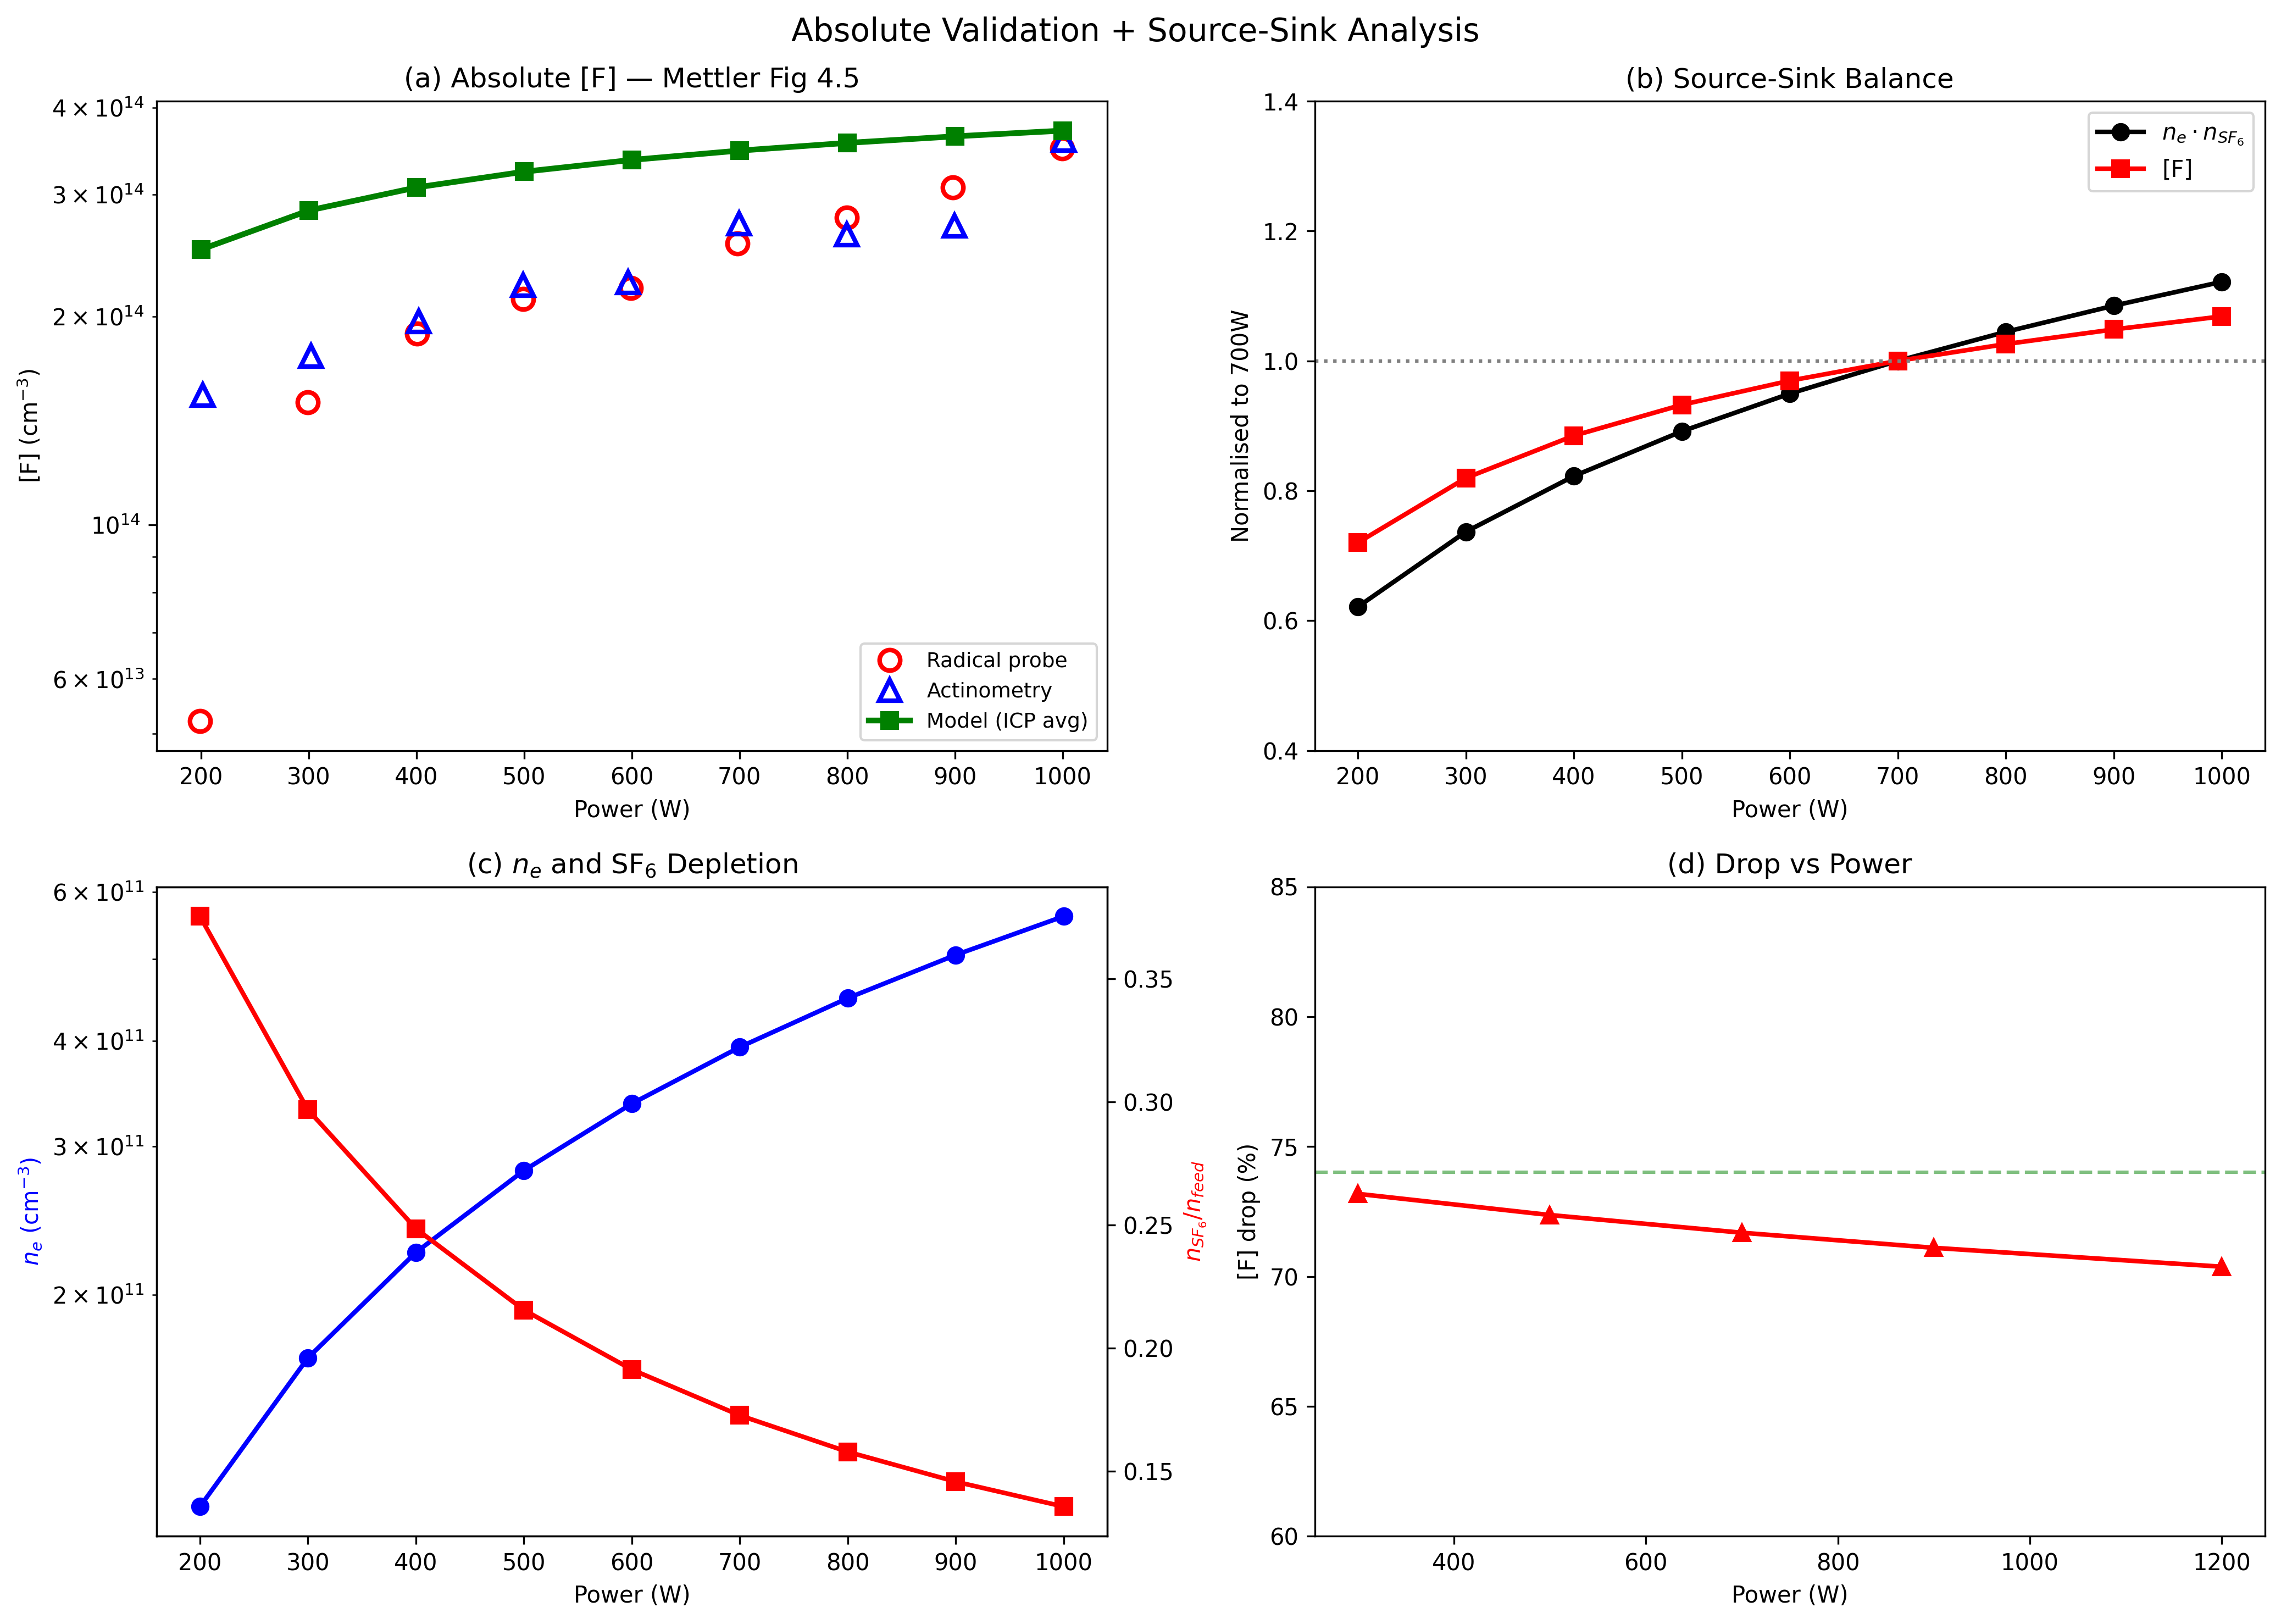
\includegraphics[width=0.65\textwidth]{absolute_validation.png}
  \caption{Summary of absolute validation metrics across all
           measured quantities.  The model captures trends
           correctly but has systematic offsets in absolute values.}
  \label{fig:abs_validation}
\end{figure}

\subsection{Solver Validation: 2D Model vs.\ 0D Lallement Reference}
\label{sec:solver_validation_0D}

To check the chemistry implementation in the 2D fluid solver
independently of the surrogate, we compare its volume-averaged
species densities against the well-established 0D global model of
\citet{lallement2009} on the same TEL geometry.  This comparison is
\emph{solver-side only} (no surrogate involved): both curves are
solver outputs, plotted across power and pressure sweeps for
neutral species (Figure~\ref{fig:solver_val_neutrals}) and charged
species (Figure~\ref{fig:solver_val_charged}).  In each panel,
solid curves are the 2D TEL model and dashed curves are the 0D
Lallement reference.  Agreement across all nine neutral species and
the principal charged-species channels confirms that the 2D
chemistry network is consistent with the established reduced model
within reactor-averaged uncertainties.

\begin{figure}[H]
  \centering
  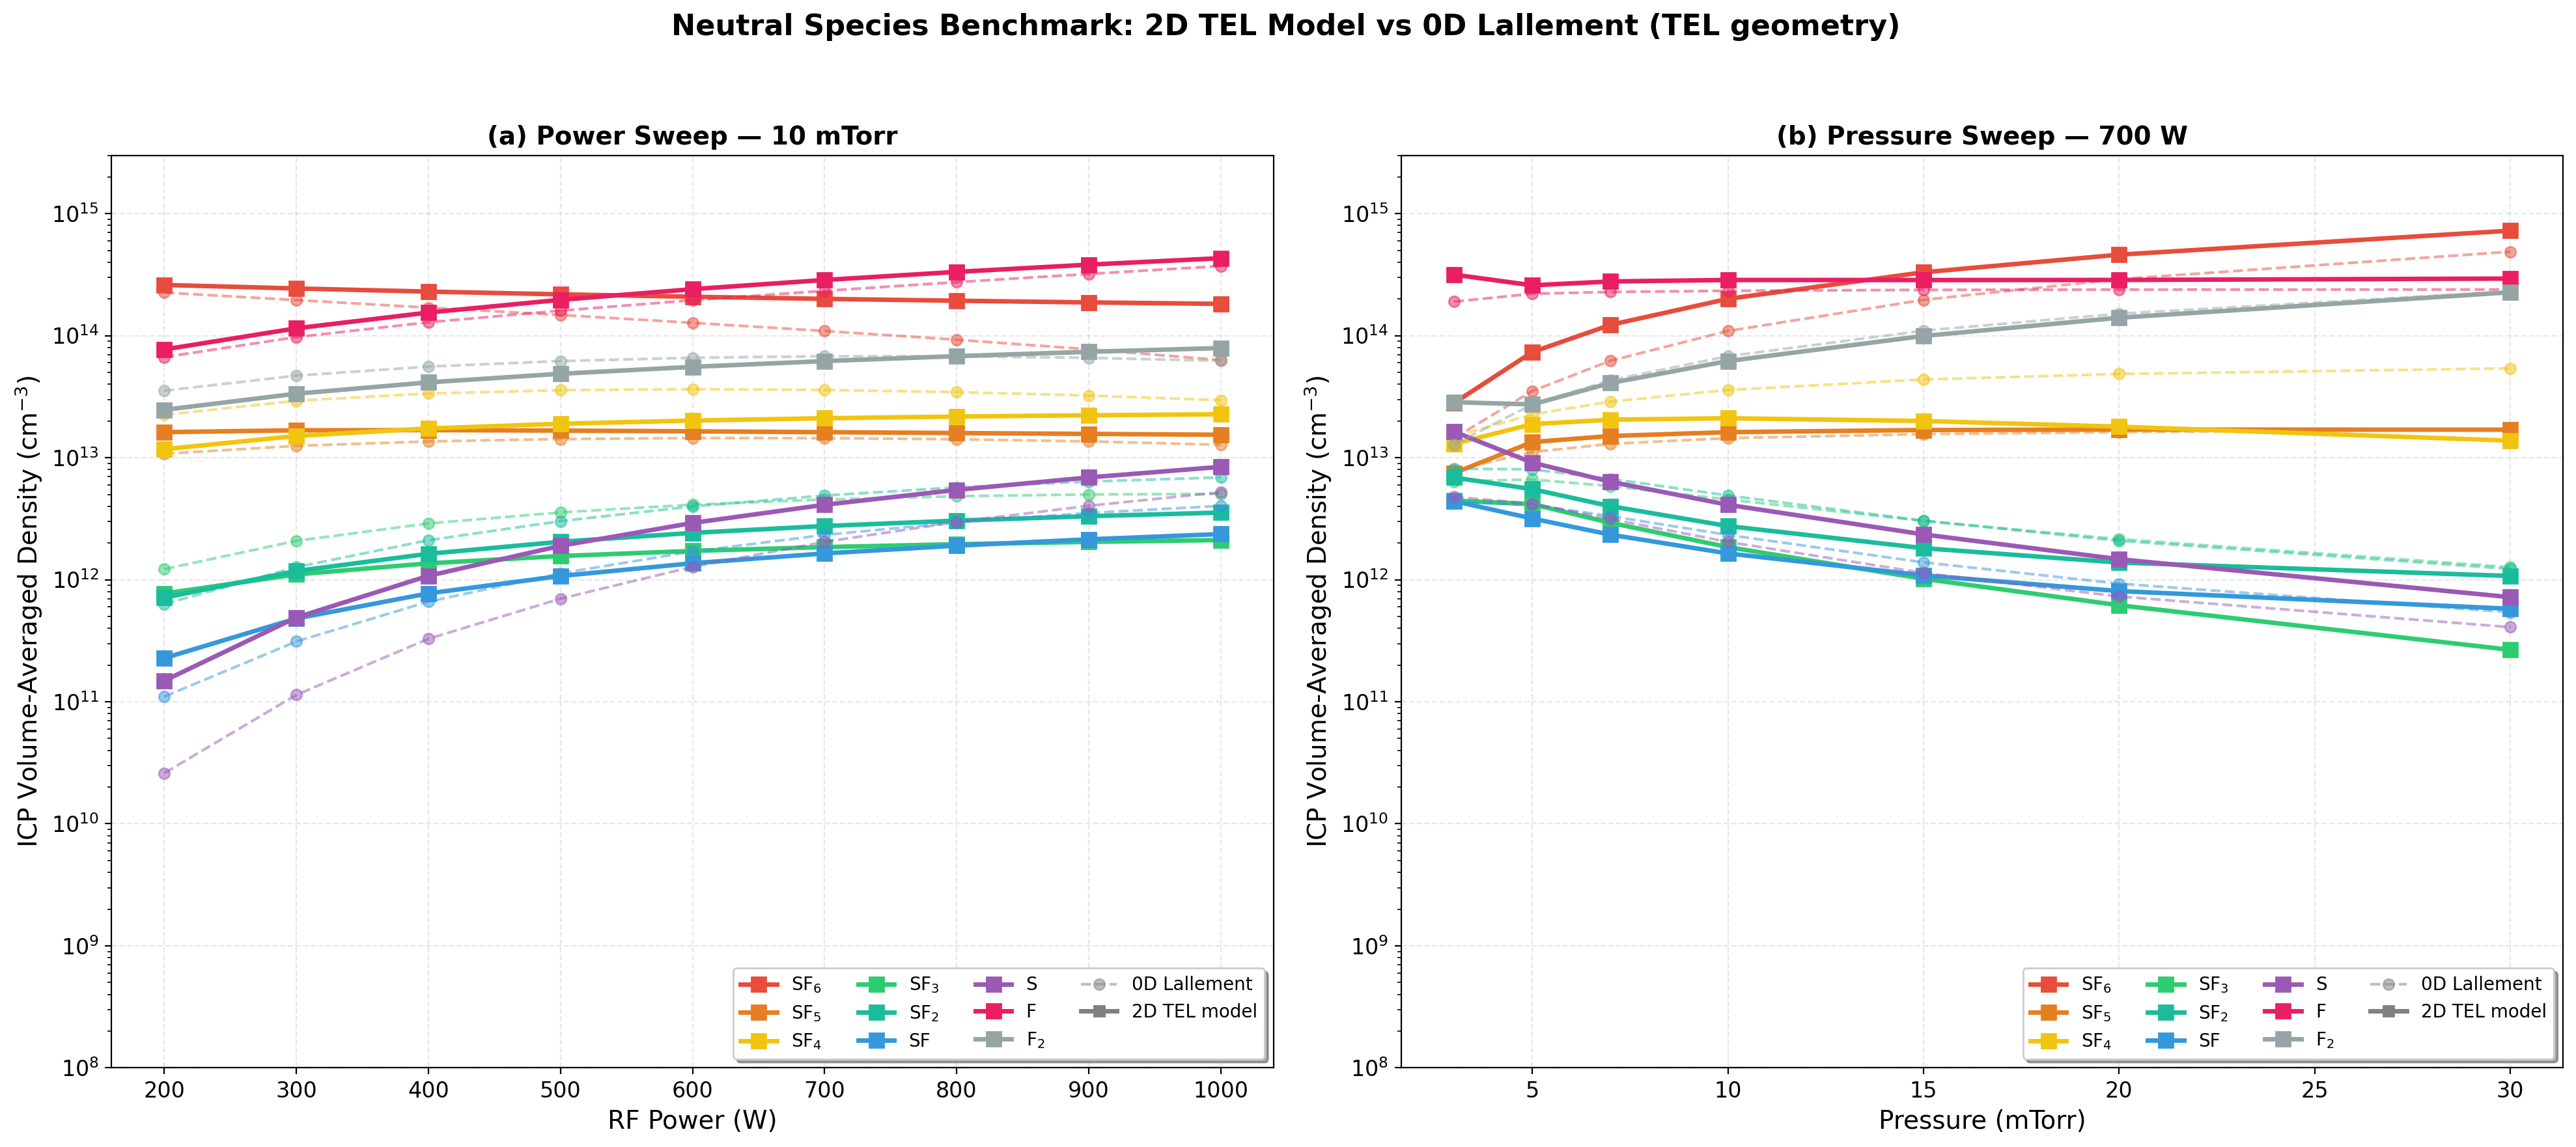
\includegraphics[width=\textwidth]{benchmark_neutrals.png}
  \caption{Solver validation for neutral species: 2D TEL fluid
           model (solid) compared to the 0D Lallement reference
           (dashed) across power and pressure sweeps.  All nine
           neutrals (SF\textsubscript{6}, SF\textsubscript{5},
           SF\textsubscript{4}, SF\textsubscript{3},
           SF\textsubscript{2}, SF, F, F\textsubscript{2}, S) shown
           on a common log-density axis.  This is solver-vs-solver,
           not surrogate-vs-solver --- the surrogate predicts only
           nF and nSF\textsubscript{6} (Figure~\ref{fig:benchmarks}
           and Section~\ref{sec:limitations}).}
  \label{fig:solver_val_neutrals}
\end{figure}

\begin{figure}[H]
  \centering
  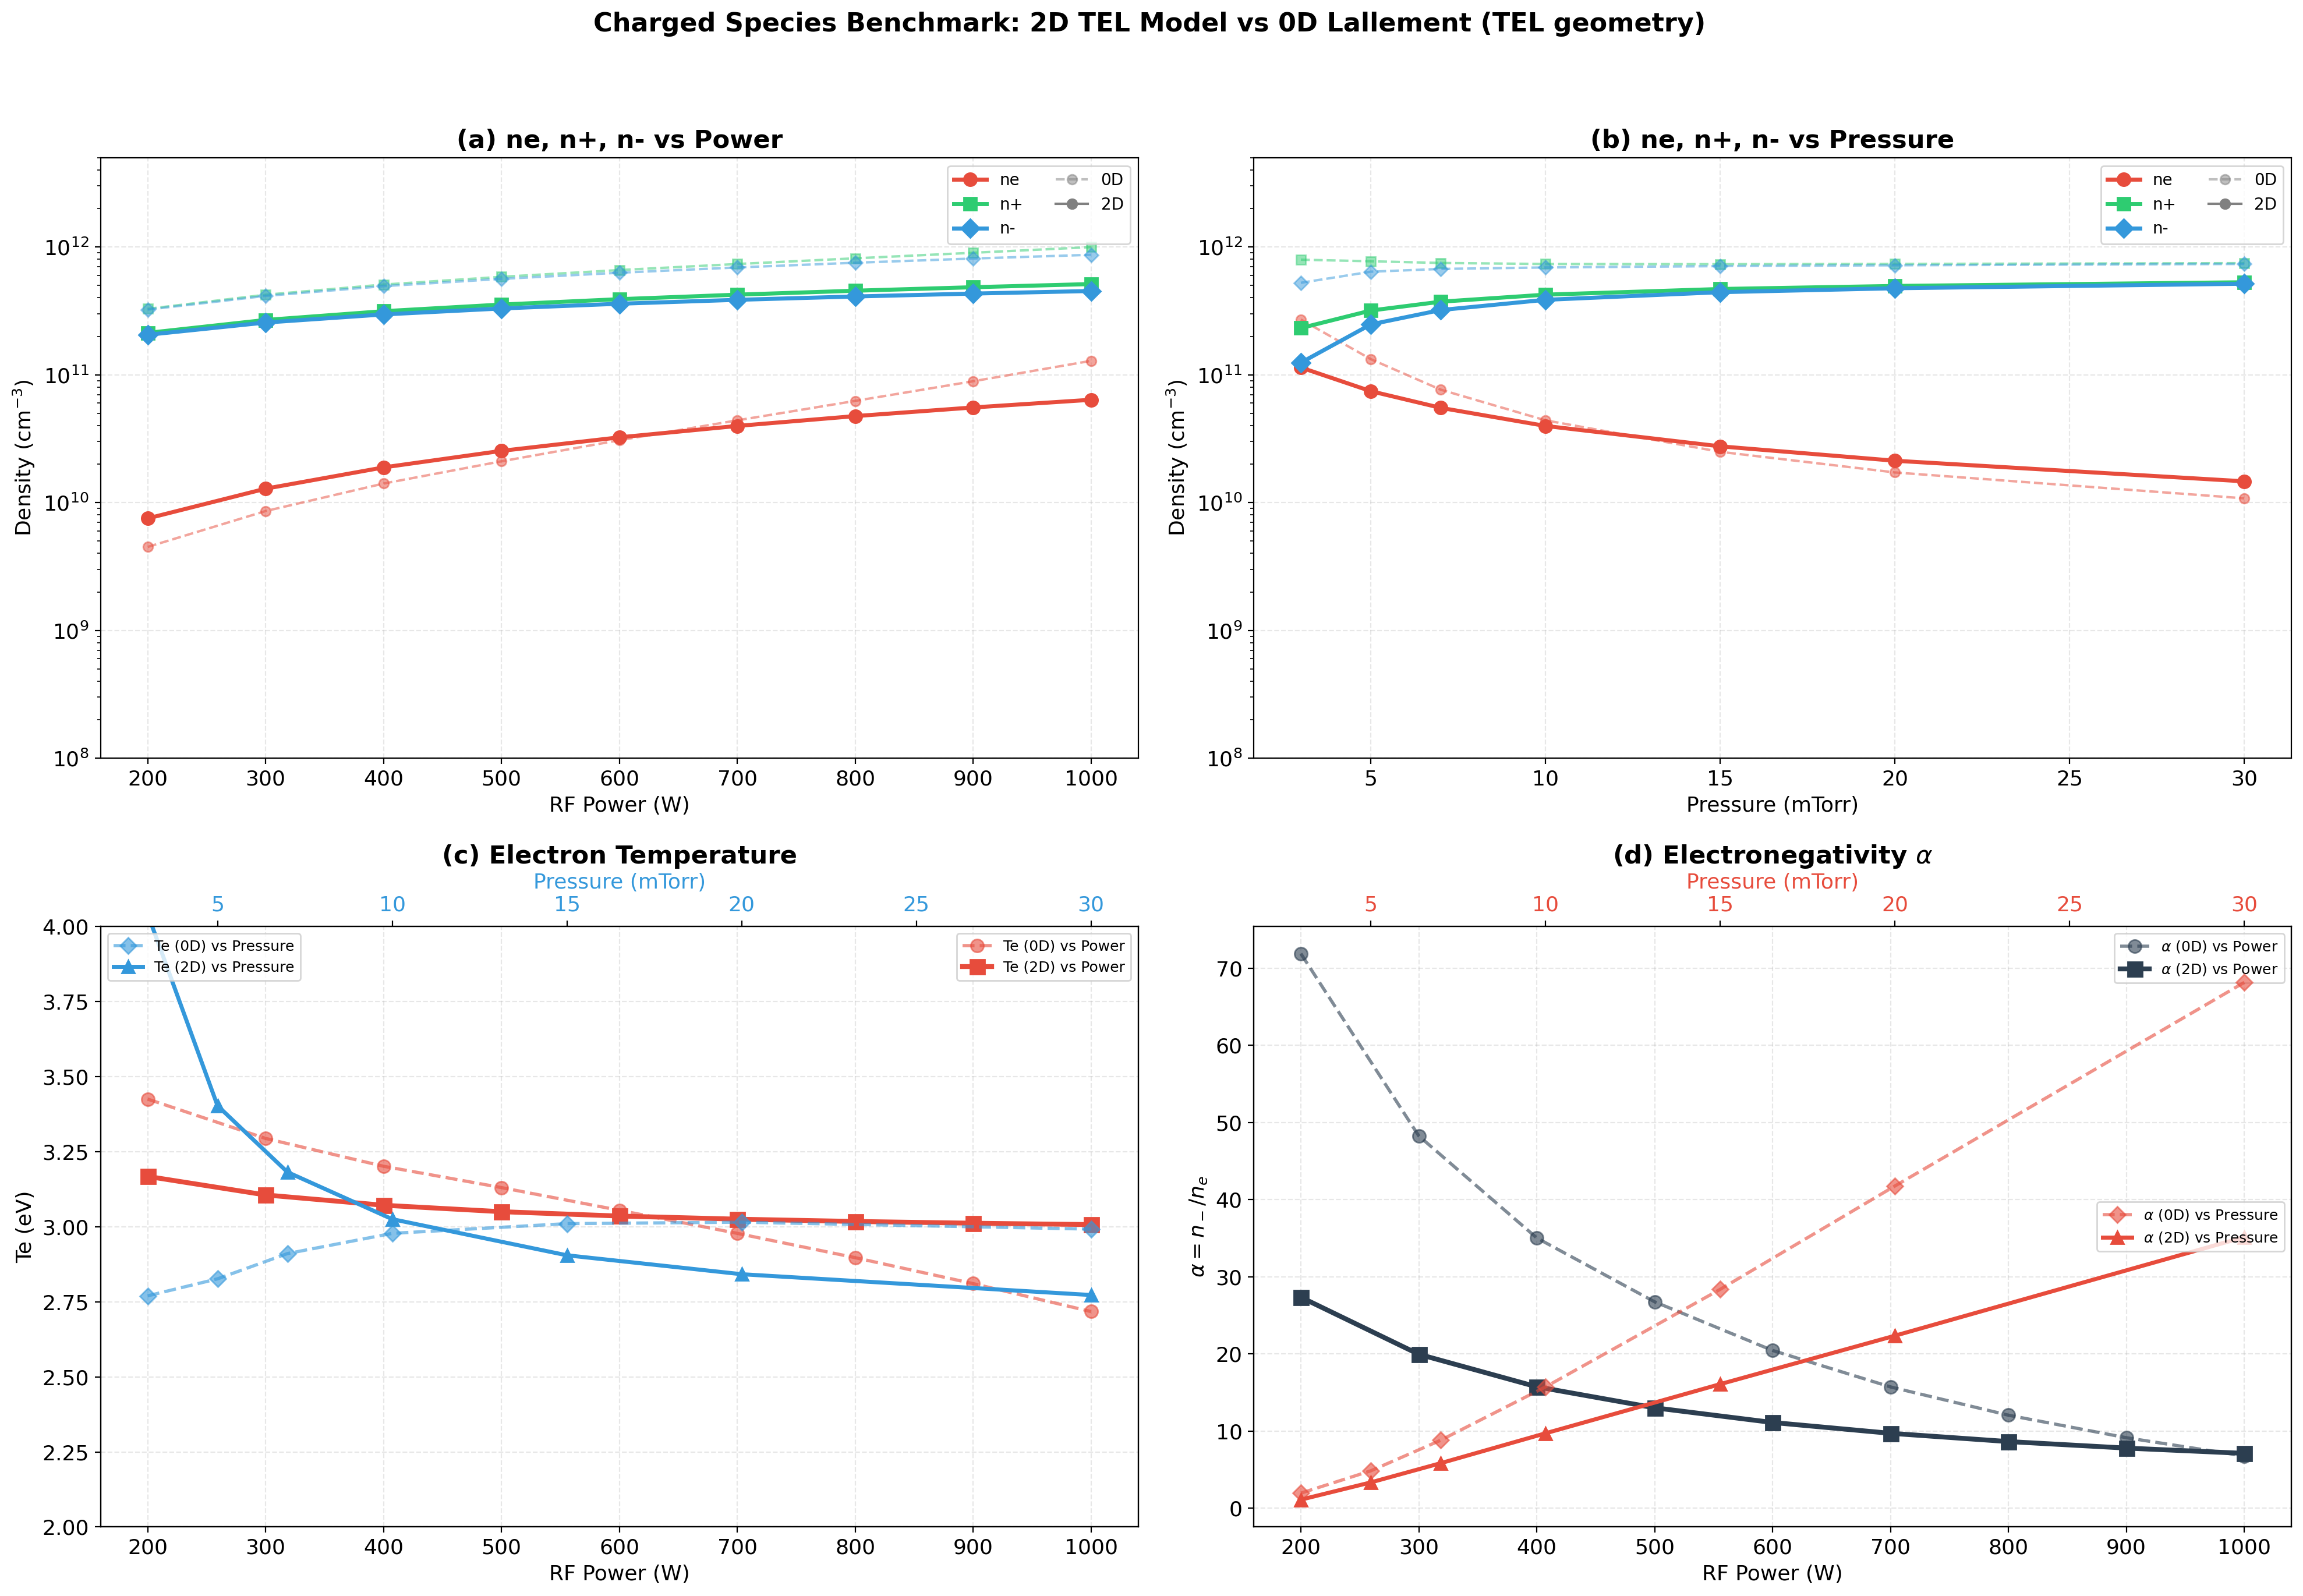
\includegraphics[width=\textwidth]{benchmark_charged.png}
  \caption{Solver validation for charged species: 2D TEL model
           (solid) vs.\ 0D Lallement reference (dashed) for
           electron density $n_e$, total positive ion density
           $n_+$, total negative ion density $n_-$, electron
           temperature $T_e$, and electronegativity $\alpha = n_-/n_e$.
           Power and pressure sweeps shown.  As above, this is a
           2D-vs-0D solver consistency check; the surrogate does
           not predict charged species.}
  \label{fig:solver_val_charged}
\end{figure}

\subsection{ML Baselines}

Table~\ref{tab:baselines} compares the MLP ensemble to classical
machine-learning baselines.

\begin{table}[H]
  \centering
  \caption{Comparison of surrogate approaches (nF RMSE).}
  \label{tab:baselines}
  \begin{tabular}{lc}
    \toprule
    Method & nF RMSE \\
    \midrule
    Polynomial (degree 3)          & 0.051  \\
    Polynomial (degree 4)          & 0.039  \\
    Gaussian Process (3000 points) & 0.006  \\
    MLP ensemble (this work)       & 0.0038 \\
    \bottomrule
  \end{tabular}
\end{table}

The MLP ensemble outperforms all baselines.  The Gaussian process
(nF RMSE = 0.006) is competitive on this metric but limited to small
training sets due to cubic scaling.  Degree-4 polynomials
(nF RMSE = 0.039) are $\sim$10$\times$ worse than the production
ensemble.

\subsection{Speedup}
\label{sec:speedup}

Table~\ref{tab:speedup} summarises the wall-clock speedup of the
production surrogate against both reference solvers.  Per-evaluation
times are averaged over 40 randomly-sampled operating conditions on
identical hardware, so the comparison isolates the cost of the inference
forward pass against the cost of the corresponding fluid-solver
integration.

\begin{table}[H]
  \centering
  \caption{Solver vs.\ surrogate wall-clock times for a single
operating-point evaluation.  The two solvers differ only in the
electron-impact rate-coefficient set; the surrogate is the same
5-model E3\_separate\_heads ensemble in both rows.  Surrogate time is
the mean of 200 timed forward passes (after a 20-pass warm-up) over an
inside-mask of 1\,780 cells per operating point.}
  \label{tab:speedup}
  \begin{tabular}{lccc}
    \toprule
    Solver & Mean time & Surrogate time & Speedup \\
    \midrule
    Legacy & \SI{7.76}{\second} & \SI{14.8}{\milli\second}
           & $524\times$ \\
    LXCat  & \SI{14.4}{\second} & \SI{14.8}{\milli\second}
           & $972\times$ \\
    \bottomrule
  \end{tabular}
\end{table}

The surrogate evaluates an entire (\(P_\mathrm{rf}\), \(p\),
\(x_\mathrm{Ar}\)) operating point in under \SI{15}{\milli\second}---two
to three orders of magnitude faster than the corresponding fluid-solver
integration, depending on which cross-section set the solver uses.  This
is the principal practical contribution of the work: the cost of an
operating-point query has dropped from seconds to a few tens of
milliseconds without sacrificing the fidelity floor established in
Section~\ref{sec:validation}.

\paragraph{What the acceleration enables.}
Concretely, the speedup converts several previously expensive workflows
into interactive ones:

\begin{itemize}
  \item \textbf{Dense parameter sweeps.}  A
        $20 \times 20 \times 10 = 4000$-point sweep over
        $(P_\mathrm{rf}, p, x_\mathrm{Ar})$ takes
        $\sim$\SI{8.6}{\hour} of wall-clock with the legacy solver and
        $\sim$\SI{16}{\hour} with the LXCat solver.  The same sweep
        completes in $\sim$\SI{1}{\minute} of surrogate inference.
  \item \textbf{Inverse design and recipe optimisation.}  Gradient-free
        optimisers (CMA-ES, Bayesian optimisation) typically need
        $10^3$--$10^4$ forward evaluations.  At the legacy solver's
        \SI{7.76}{\second} per call this is days of compute; with the
        surrogate it is seconds, opening the door to closed-loop recipe
        tuning against an experimental cost function.
  \item \textbf{Real-time control and digital-twin use.}  At
        \SI{14.8}{\milli\second}/eval, the surrogate is fast enough to
        sit inside a control or feedback loop running at $\sim$\SI{60}{\hertz},
        which the underlying solver categorically cannot.
  \item \textbf{Sensitivity propagation.}  Monte-Carlo propagation of
        boundary-condition or cross-section uncertainty through $10^5$
        samples is a \SI{9}{\day} job with the legacy solver and a
        \SI{25}{\minute} job with the surrogate.
\end{itemize}

The amortised cost of training the production ensemble (a few
core-hours, dominated by the architecture sweep) breaks even against
the solver after roughly 1--2 thousand surrogate evaluations.
Anything beyond a one-off operating point therefore comes out ahead.

% ==================================================================
\section{Parameter Sensitivity and Sweep Results}
\label{sec:sweeps}

To contextualise the surrogate's operating range, we present the
solver's parameter sweeps (Figures~\ref{fig:sweeps}--\ref{fig:sensitivity}).
These also serve as test cases for the surrogate.

\begin{figure}[H]
  \centering
  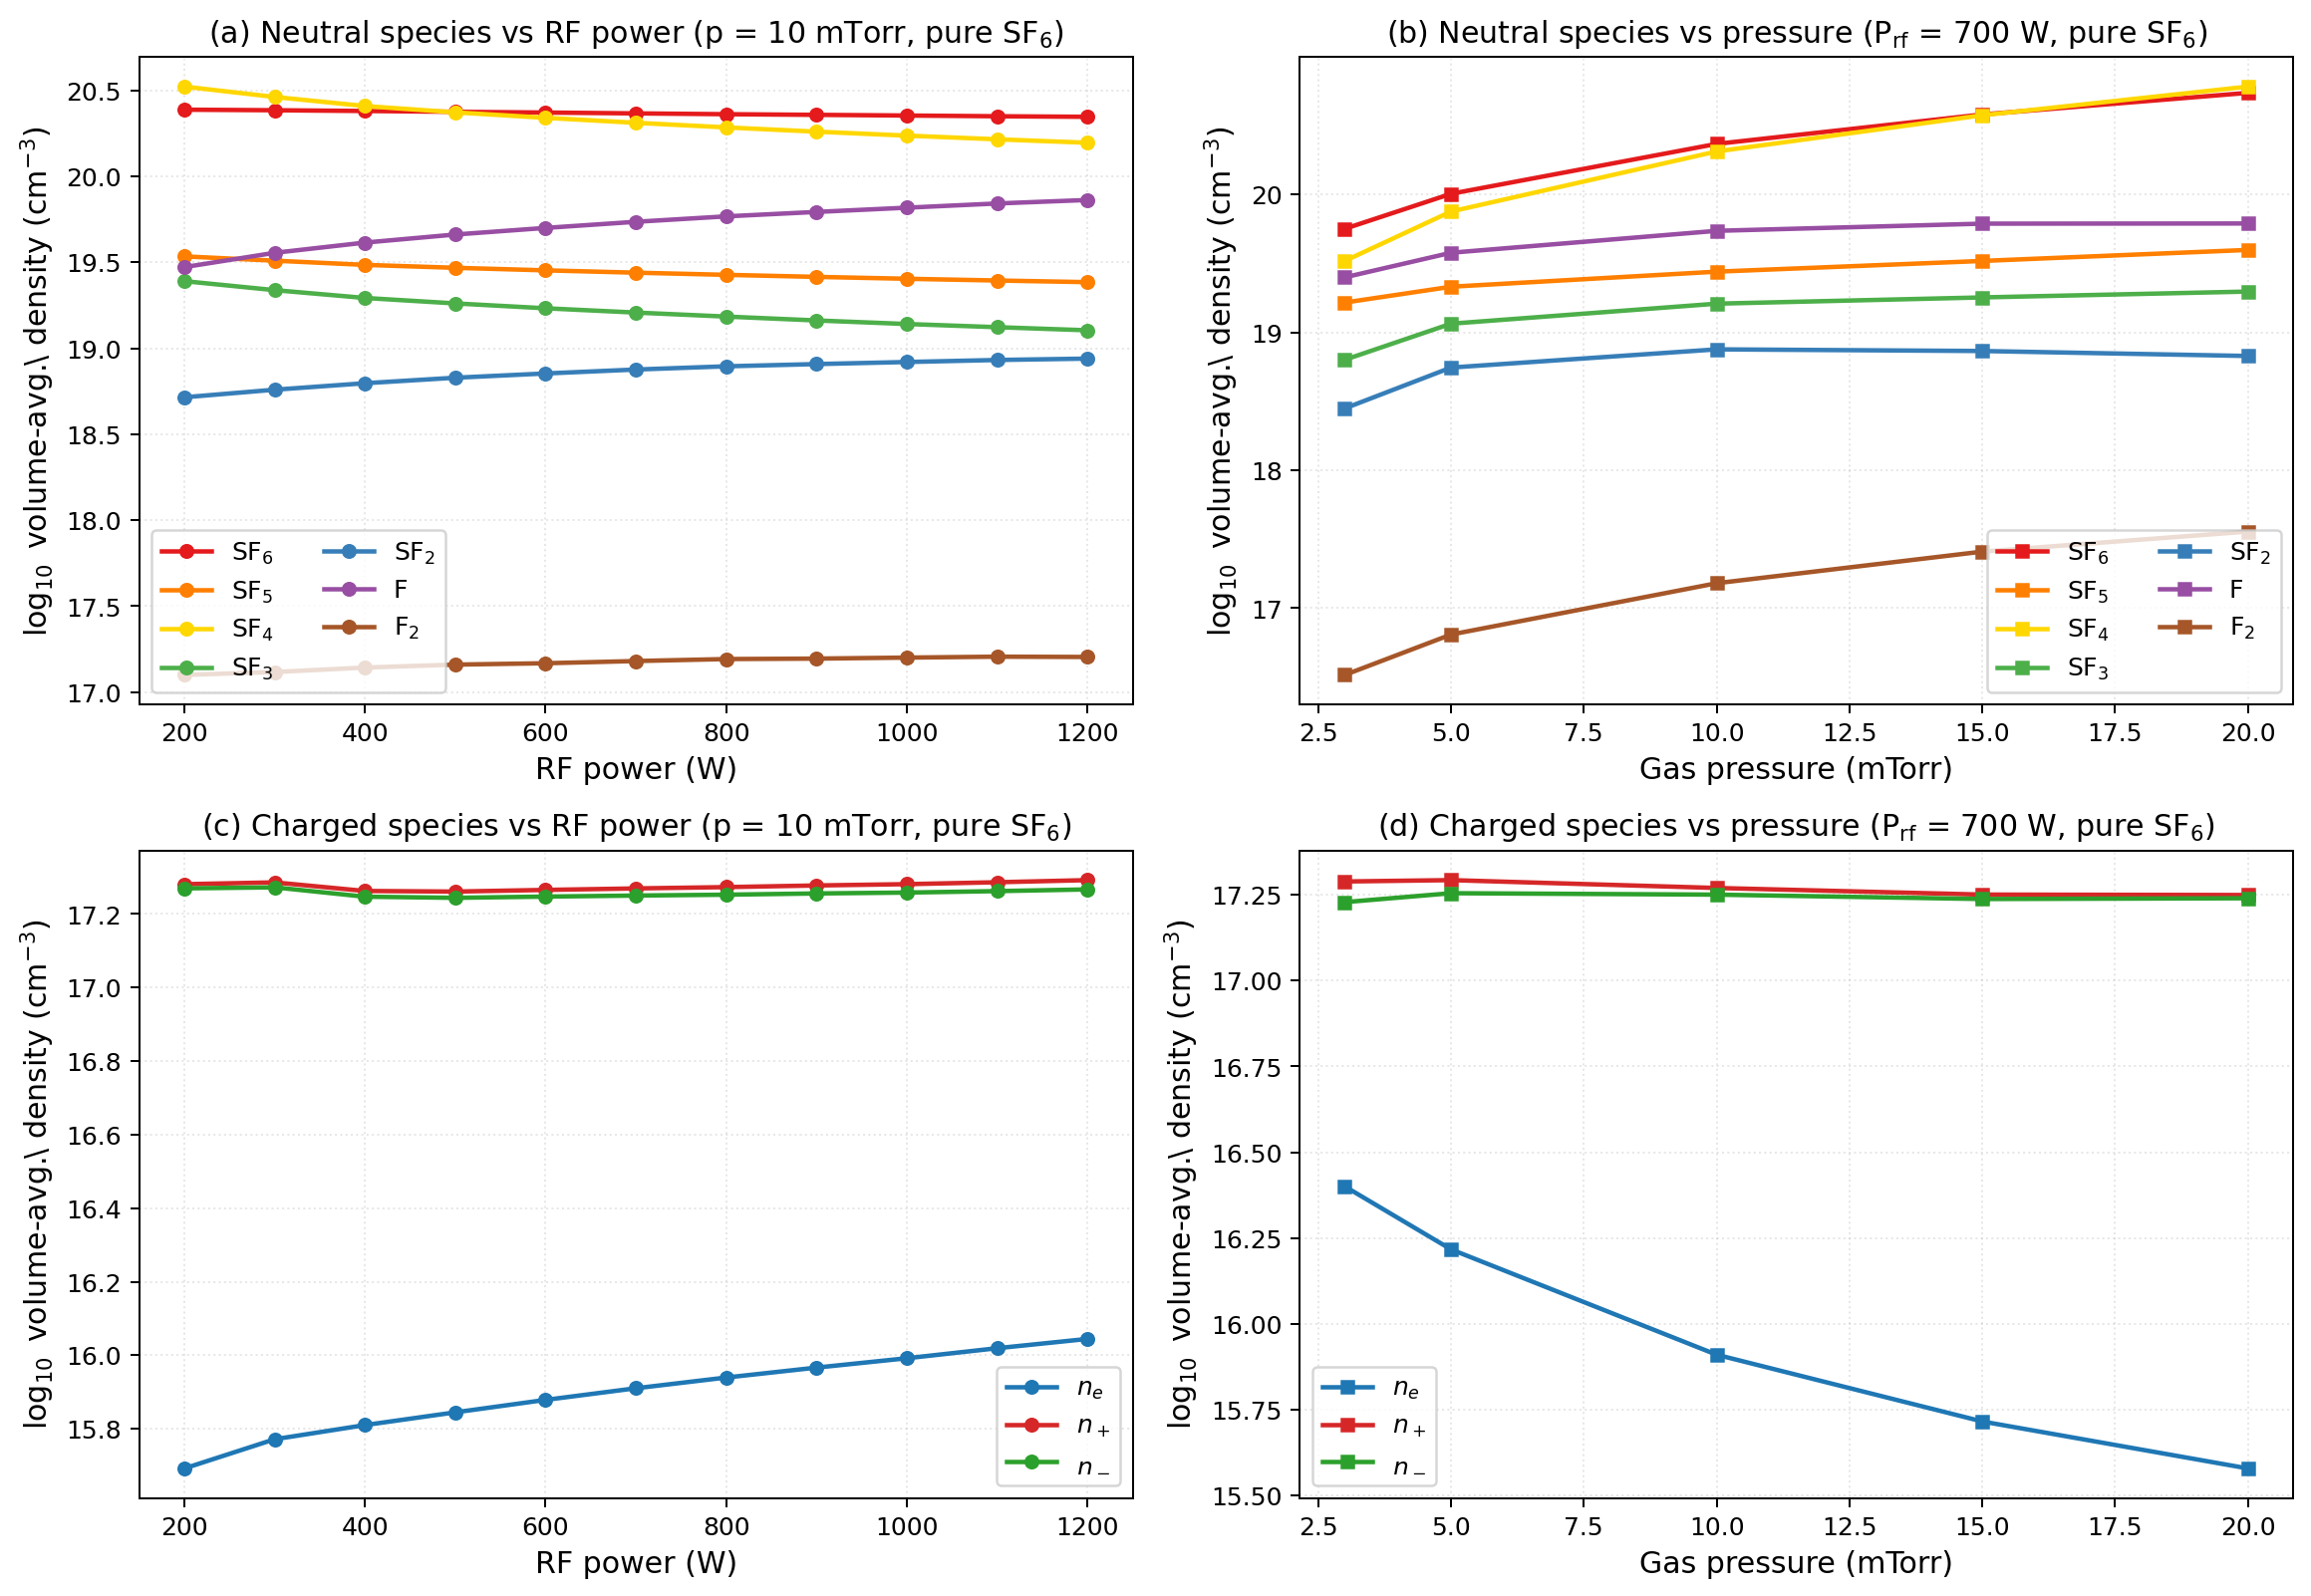
\includegraphics[width=\textwidth]{parameter_sweeps_clean.png}
  \caption{Parameter sweeps from the 2D solver.  Top row: volume-averaged
           neutral densities (SF\textsubscript{6}, SF\textsubscript{5},
           SF\textsubscript{4}, SF\textsubscript{3}, SF\textsubscript{2},
           F, F\textsubscript{2}) vs.\ RF power (a) at
           $p = 10$~mTorr and vs.\ pressure (b) at
           $P_\mathrm{rf} = \SI{700}{\watt}$.  Bottom row:
           charged-species densities ($n_e$, $n_+$, $n_-$) over the same
           power (c) and pressure (d) sweeps.  All cases are pure
           SF\textsubscript{6}; densities are volume-averaged over the
           inside-mask cells of the reactor.}
  \label{fig:sweeps}
\end{figure}

\begin{figure}[H]
  \centering
  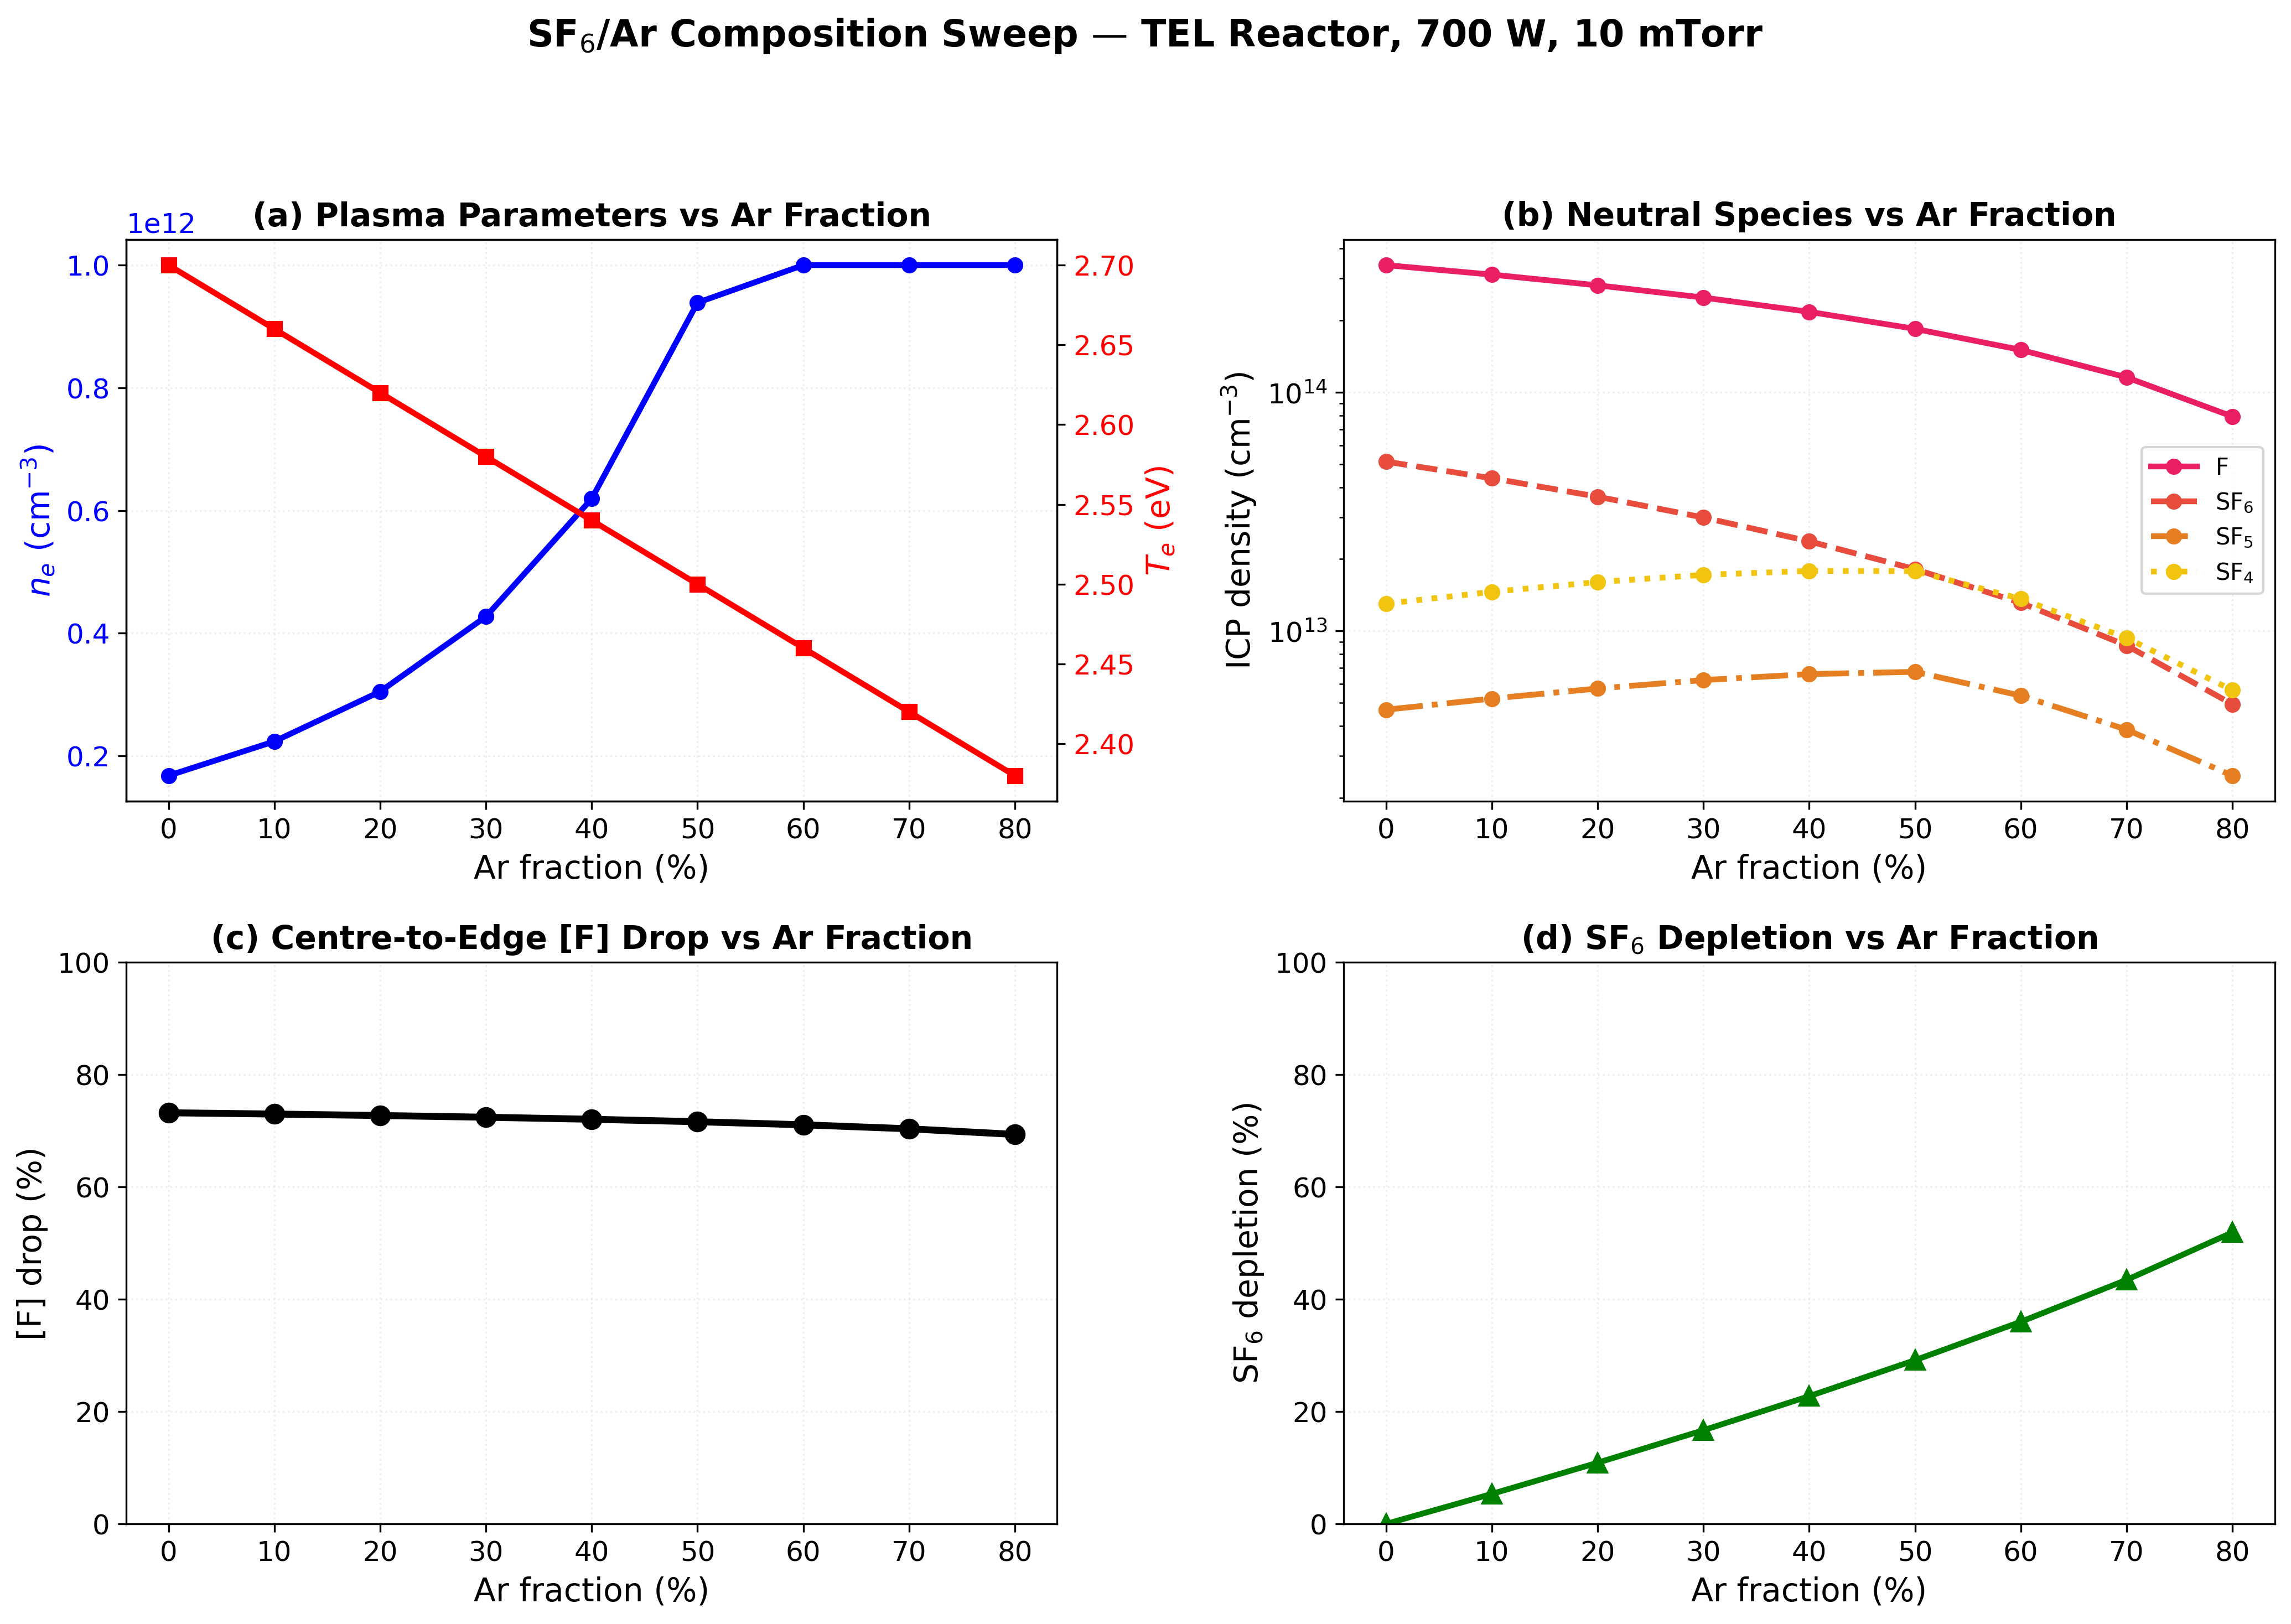
\includegraphics[width=0.65\textwidth]{composition_sweep.png}
  \caption{Effect of Ar fraction on species densities.  Increasing Ar
           dilution reduces SF\textsubscript{6} dissociation products
           while raising the electron density due to the lower
           ionisation threshold of Ar.}
  \label{fig:composition}
\end{figure}

\begin{figure}[H]
  \centering
  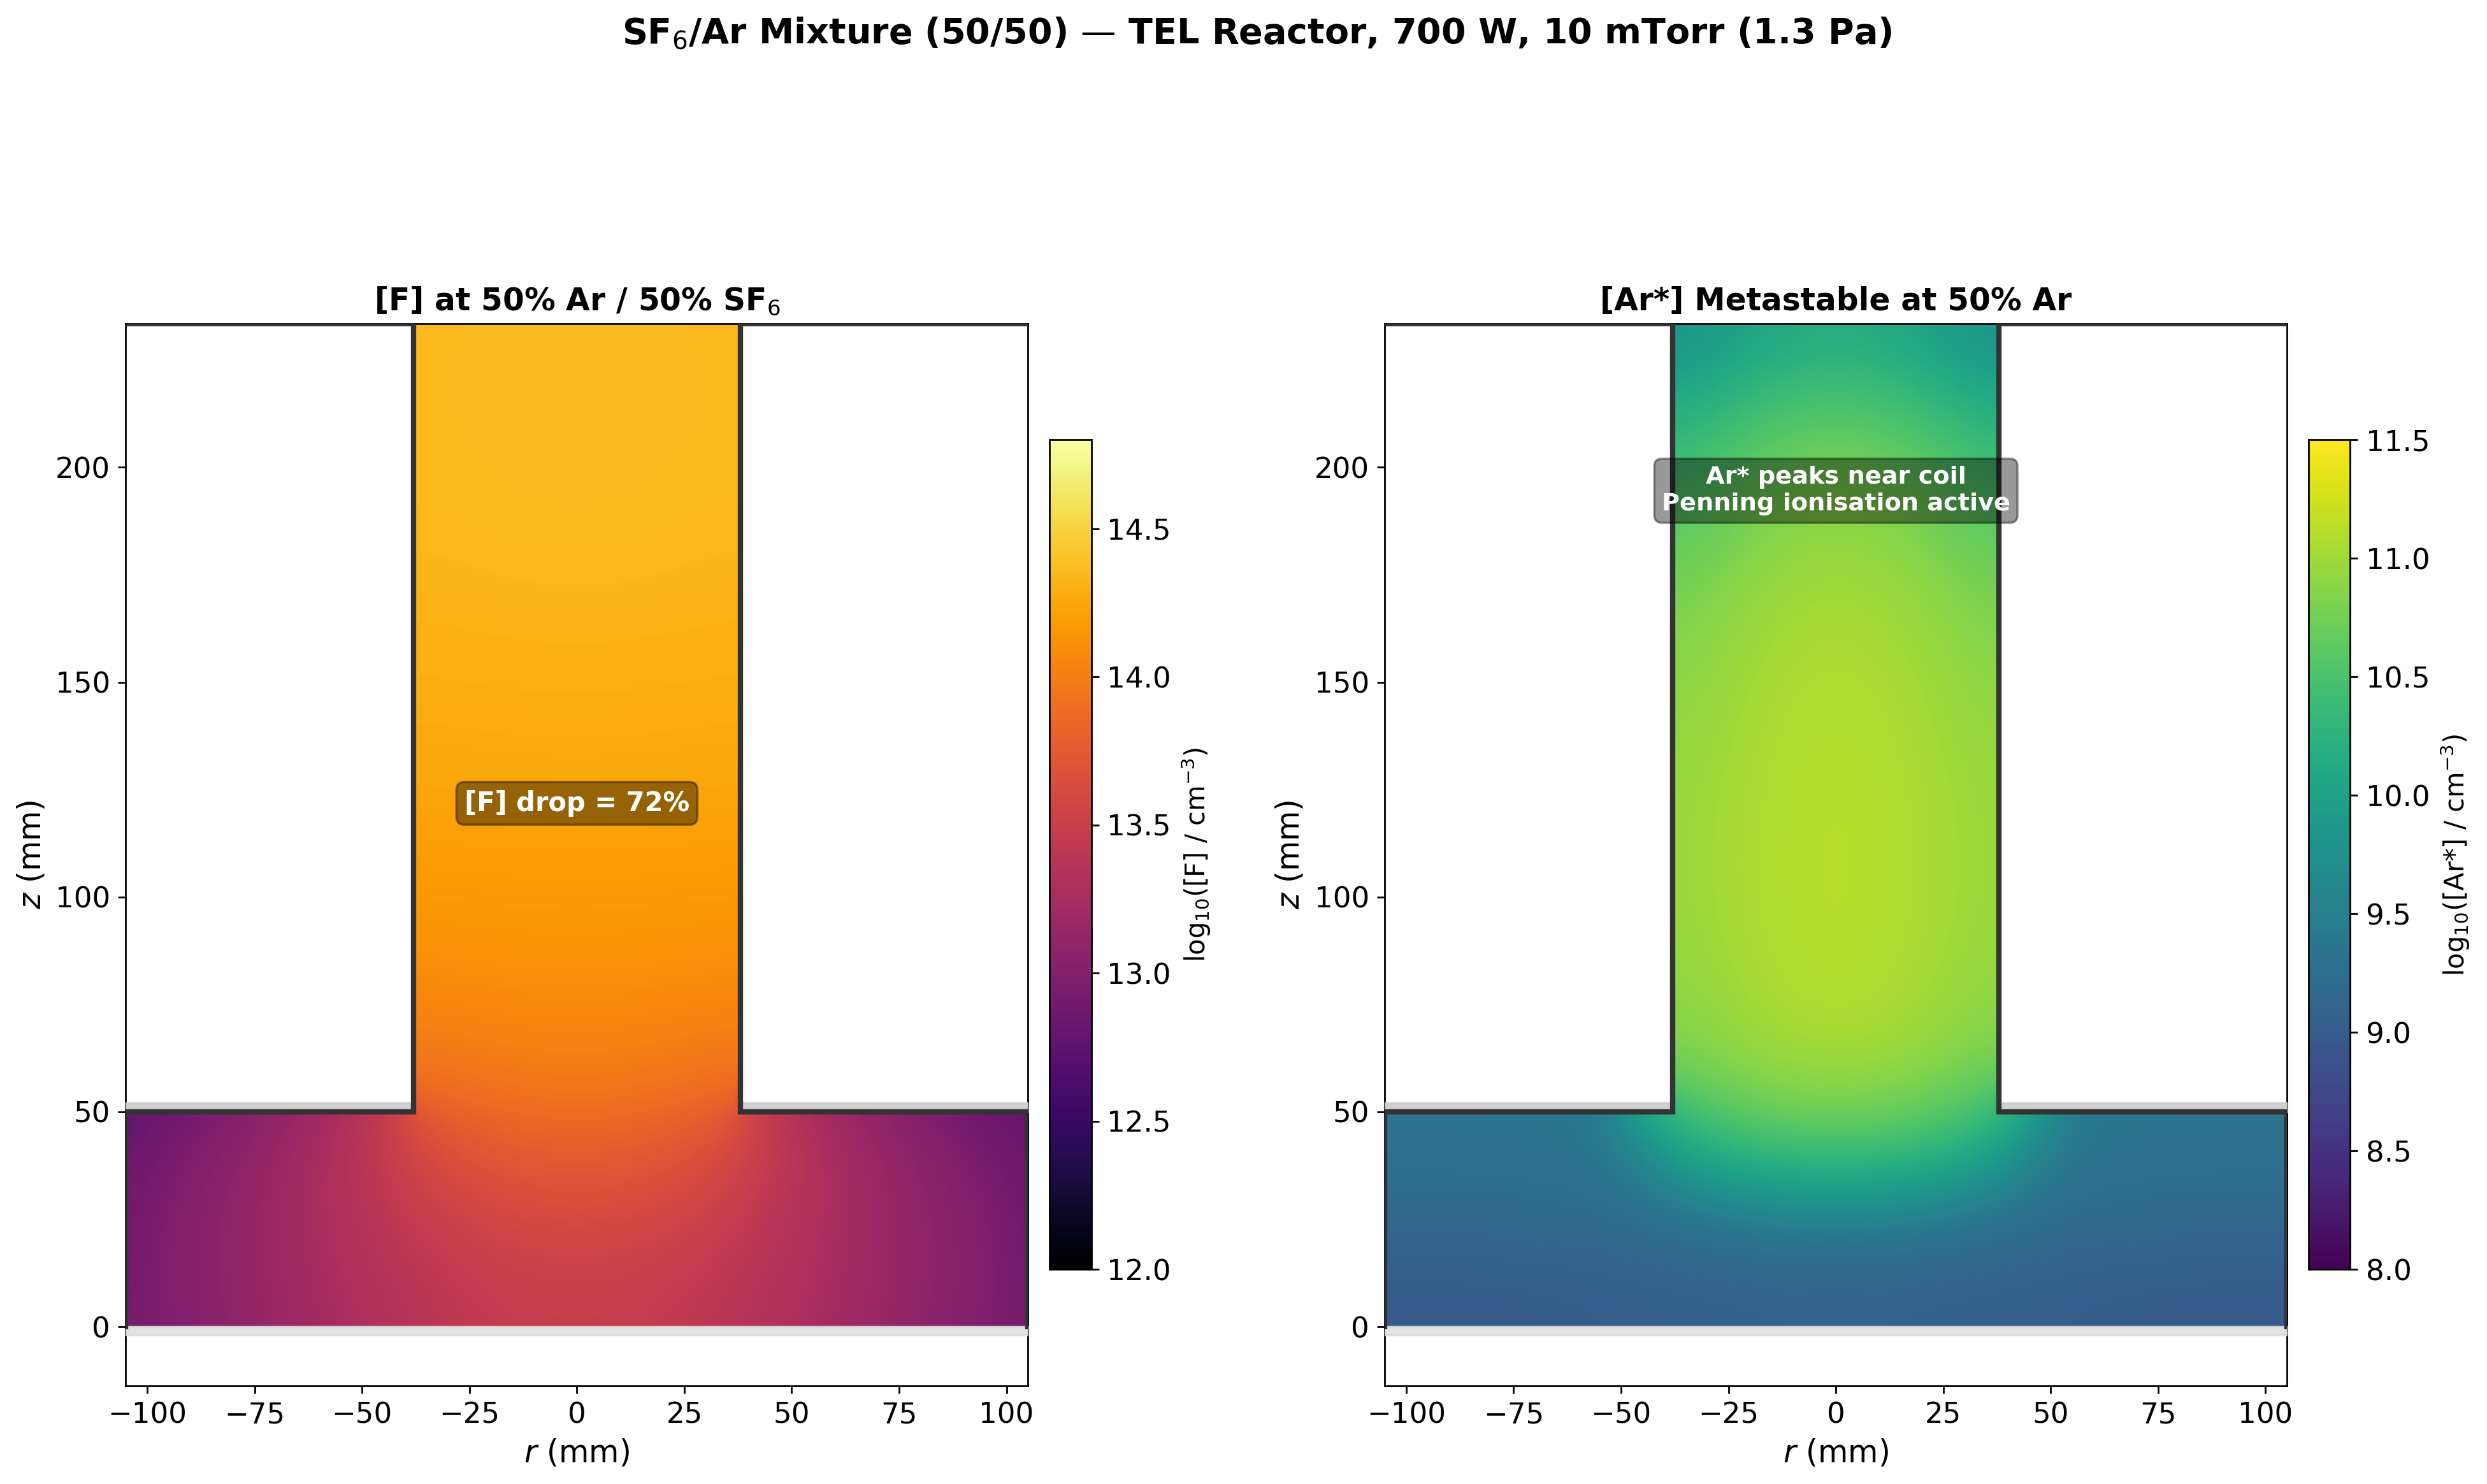
\includegraphics[width=0.65\textwidth]{Ar_contours.png}
  \caption{Spatial distribution of Ar metastable and Ar$^+$ densities
           at 30\% Ar fraction, showing the characteristic
           skin-depth confinement.}
  \label{fig:ar_contours}
\end{figure}

\begin{figure}[H]
  \centering
  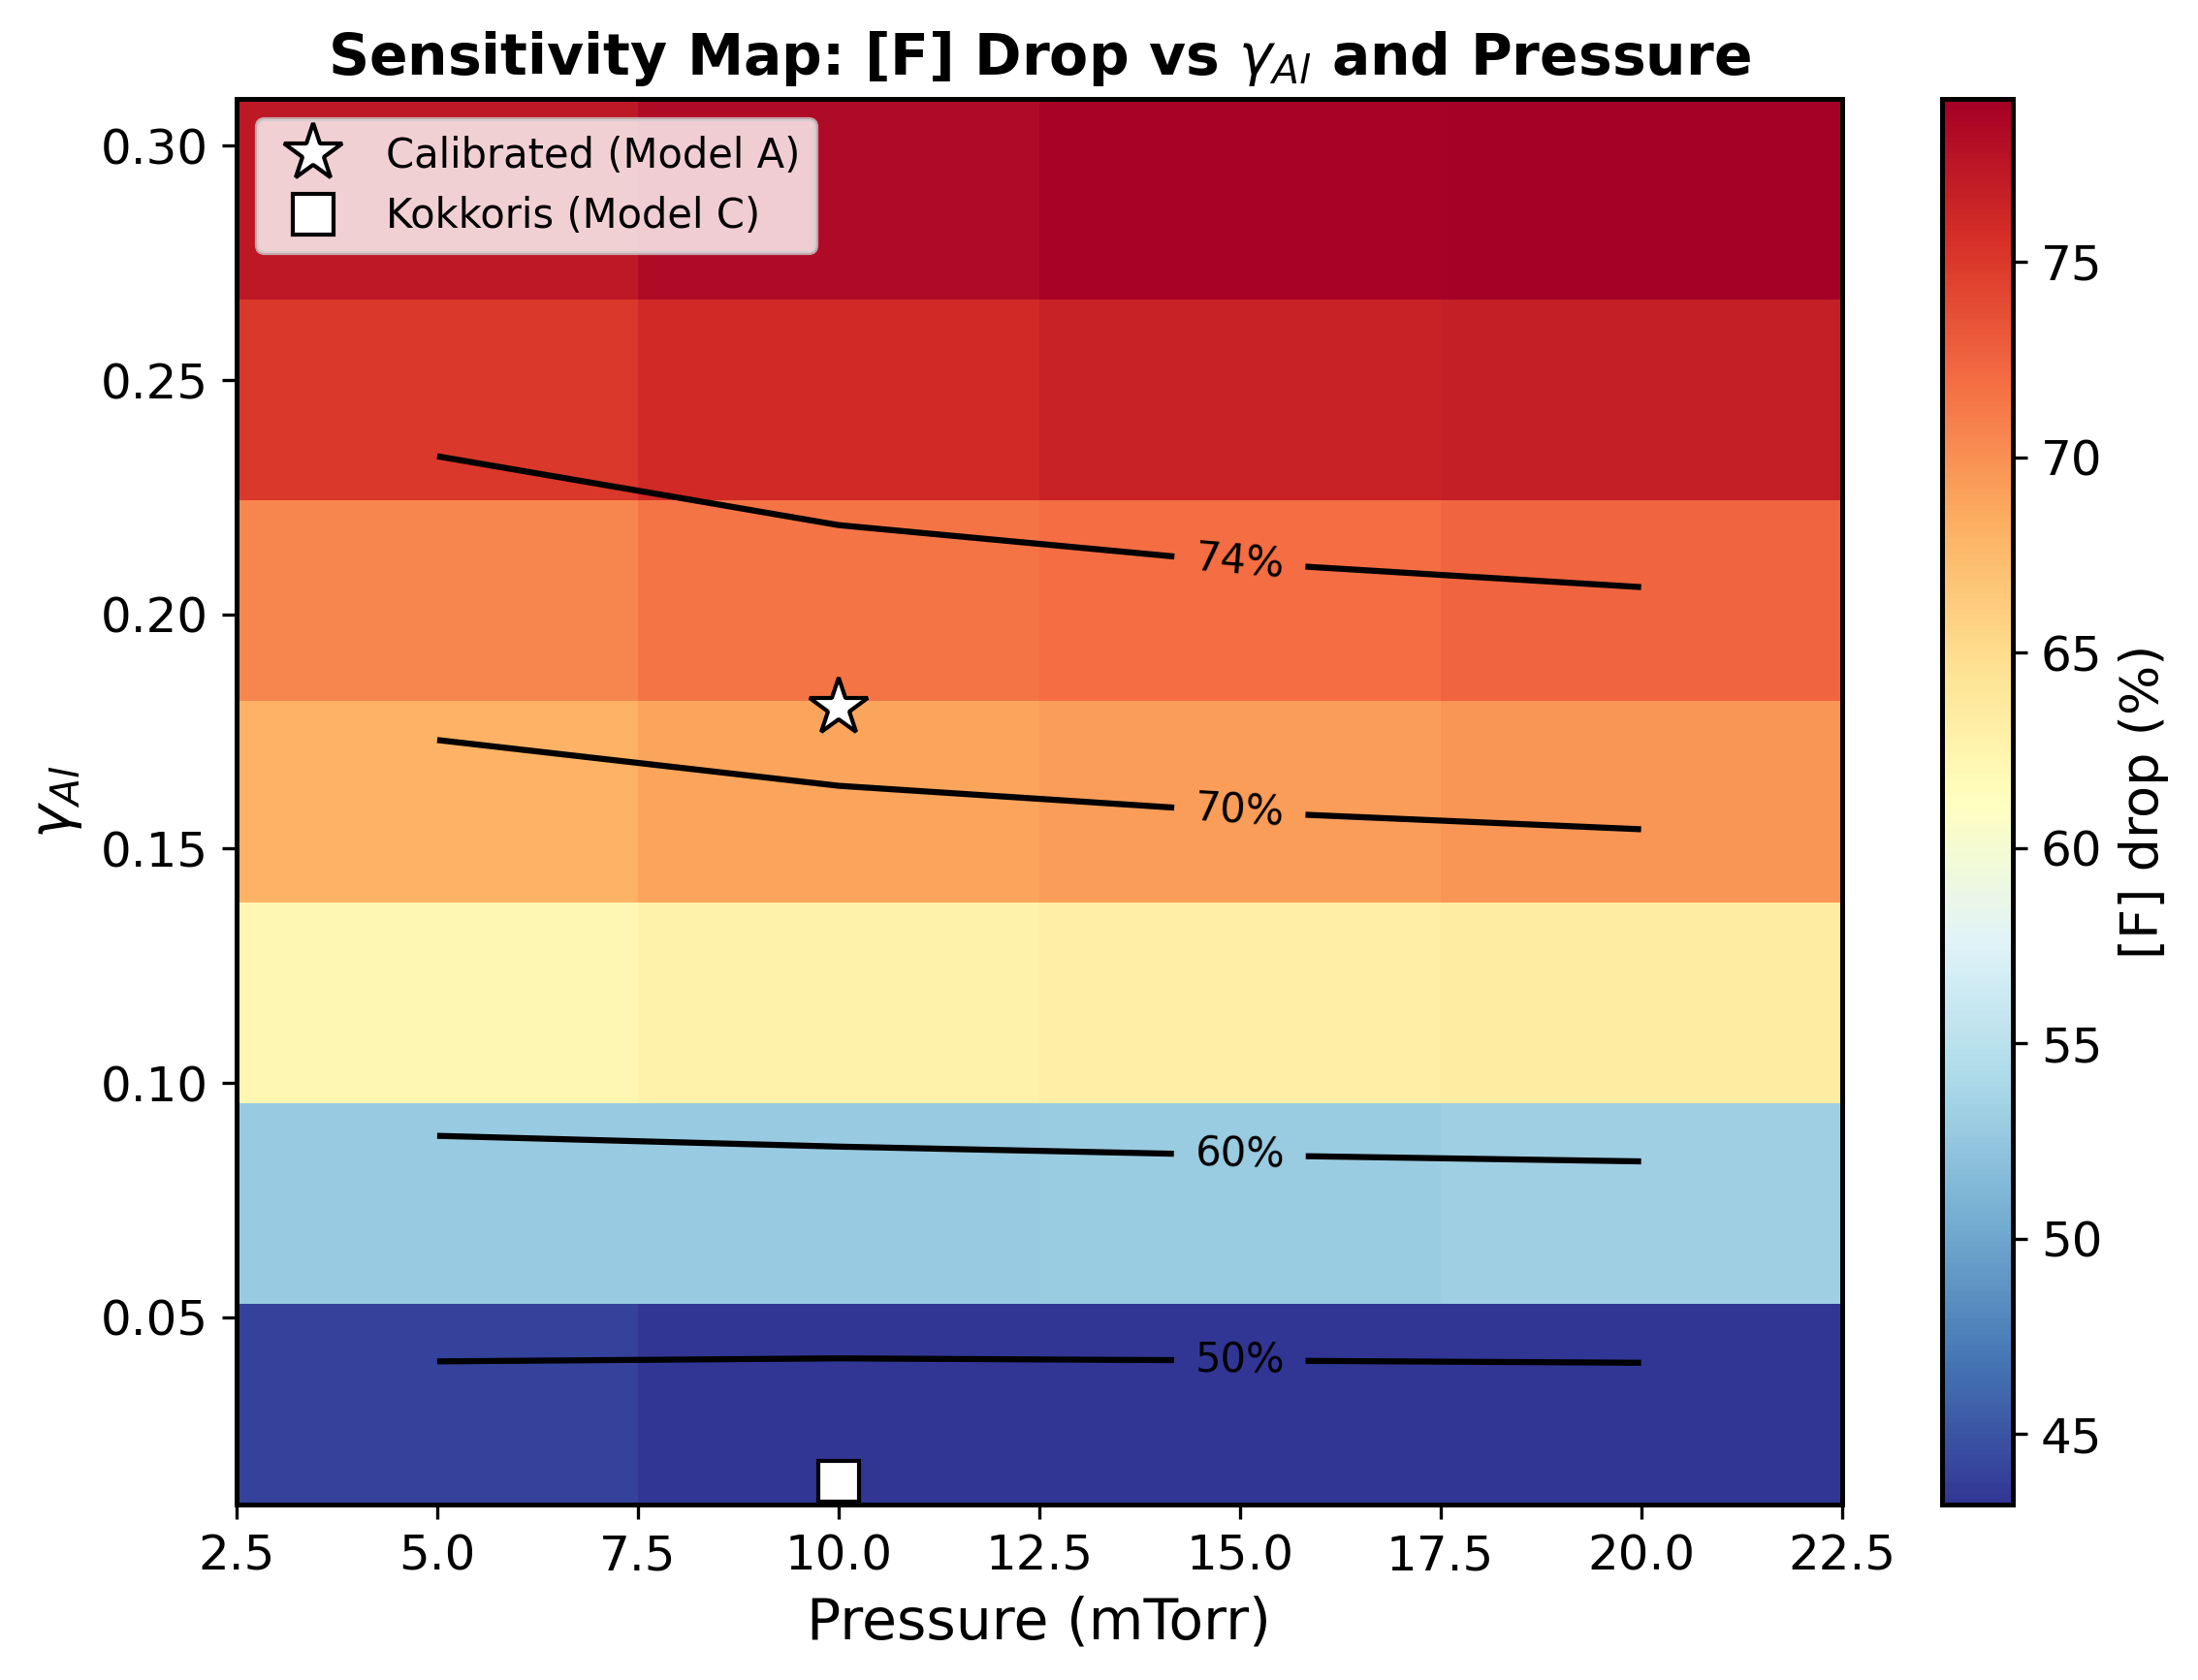
\includegraphics[width=0.65\textwidth]{sensitivity_map.png}
  \caption{Sensitivity map showing the partial derivatives
           $\partial \ln n_{\text{F}} / \partial x_i$ for each input
           parameter.  RF power and pressure dominate; Ar fraction
           has a secondary but non-negligible effect.}
  \label{fig:sensitivity}
\end{figure}

Figure~\ref{fig:wafer_diag} shows wafer-level diagnostics: the
radial F profile that governs etch uniformity and the species flux
budget at the wafer surface.

\begin{figure}[H]
  \centering
  \begin{subfigure}[t]{0.48\textwidth}
    \centering
    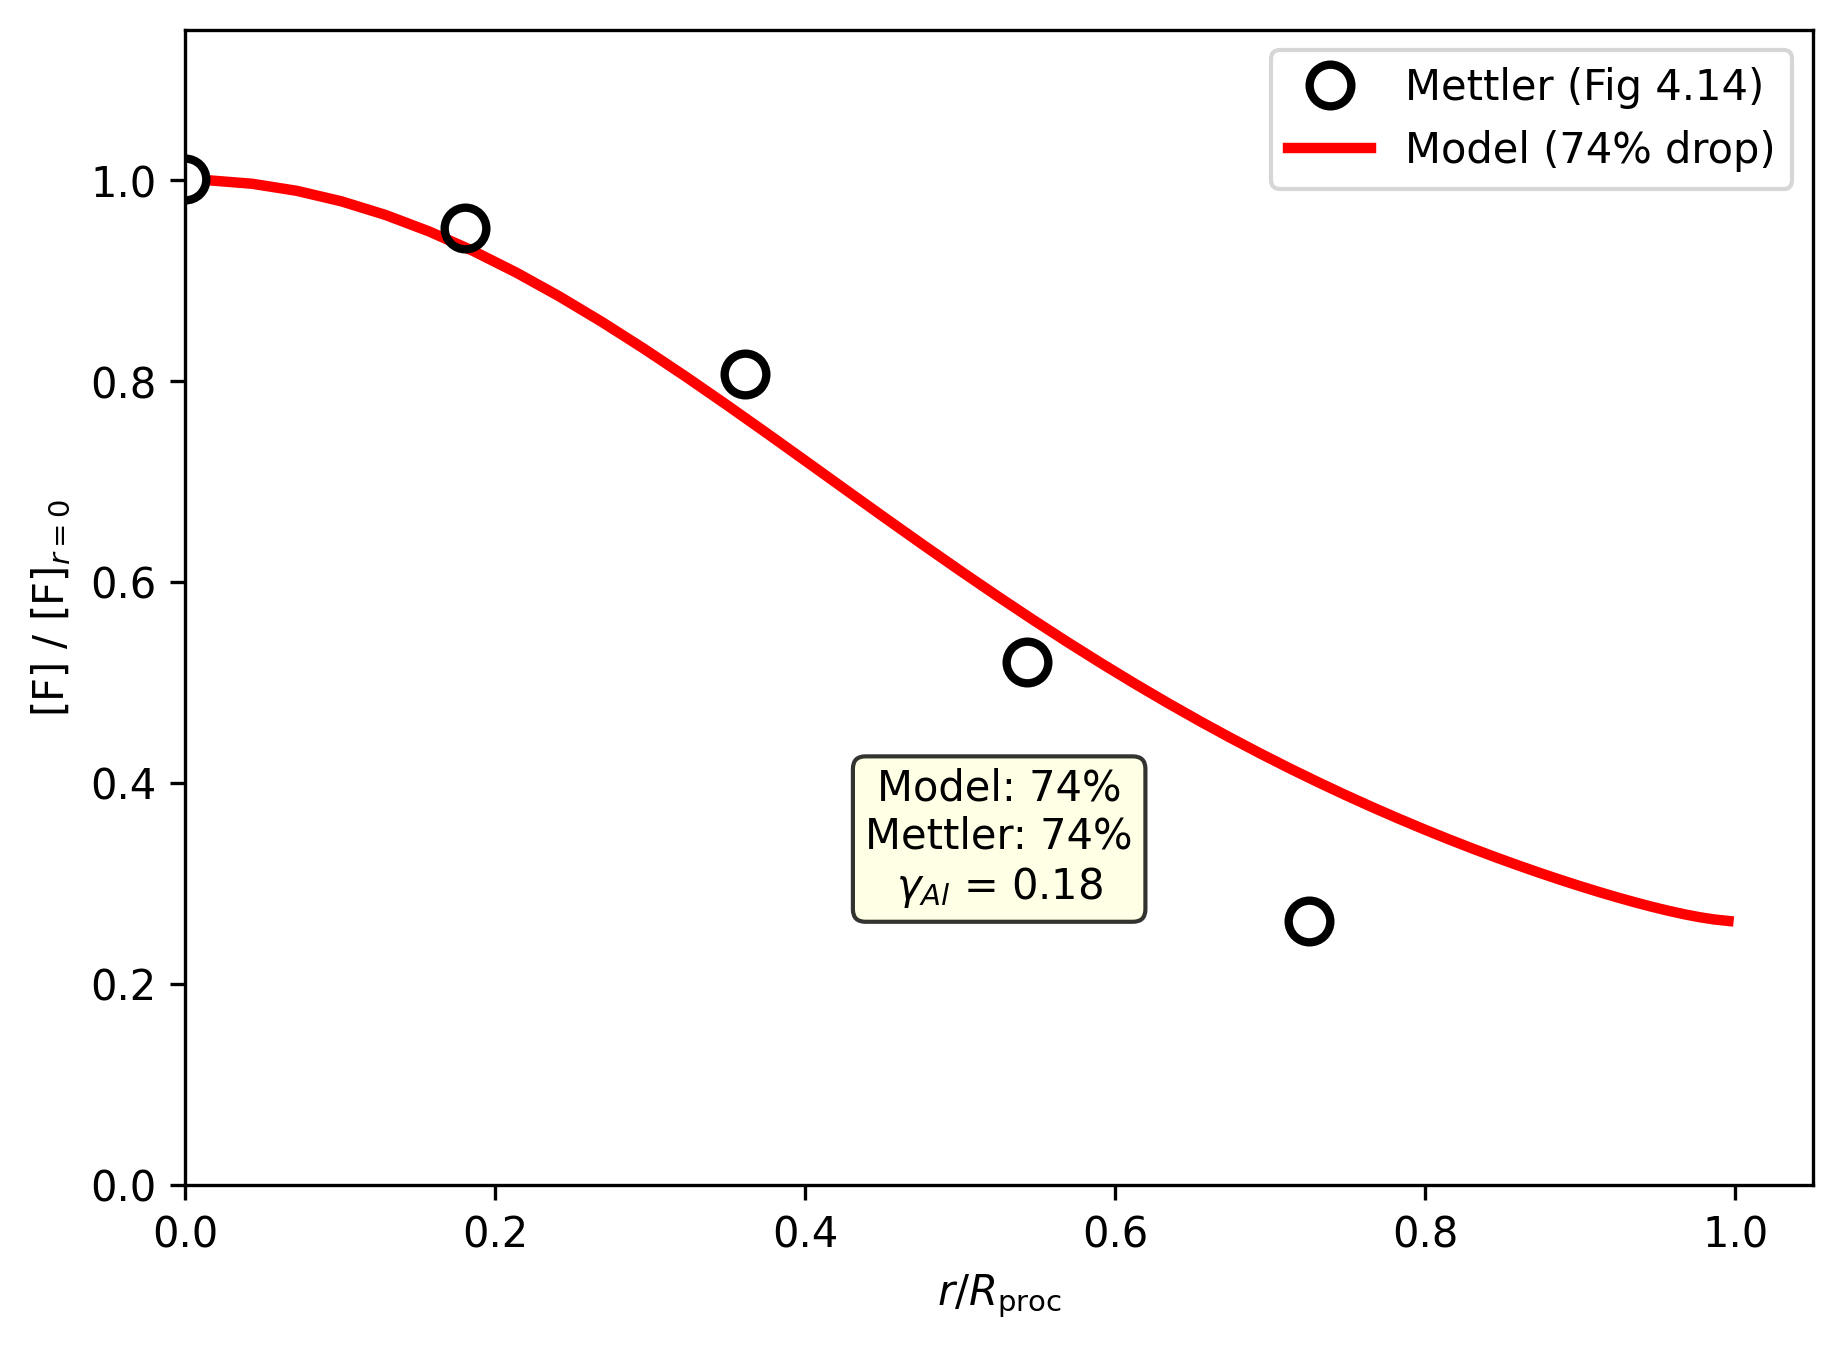
\includegraphics[width=\textwidth]{radial_F_profile.png}
    \caption{Radial F density profile at the wafer.}
    \label{fig:radial_F}
  \end{subfigure}
  \hfill
  \begin{subfigure}[t]{0.48\textwidth}
    \centering
    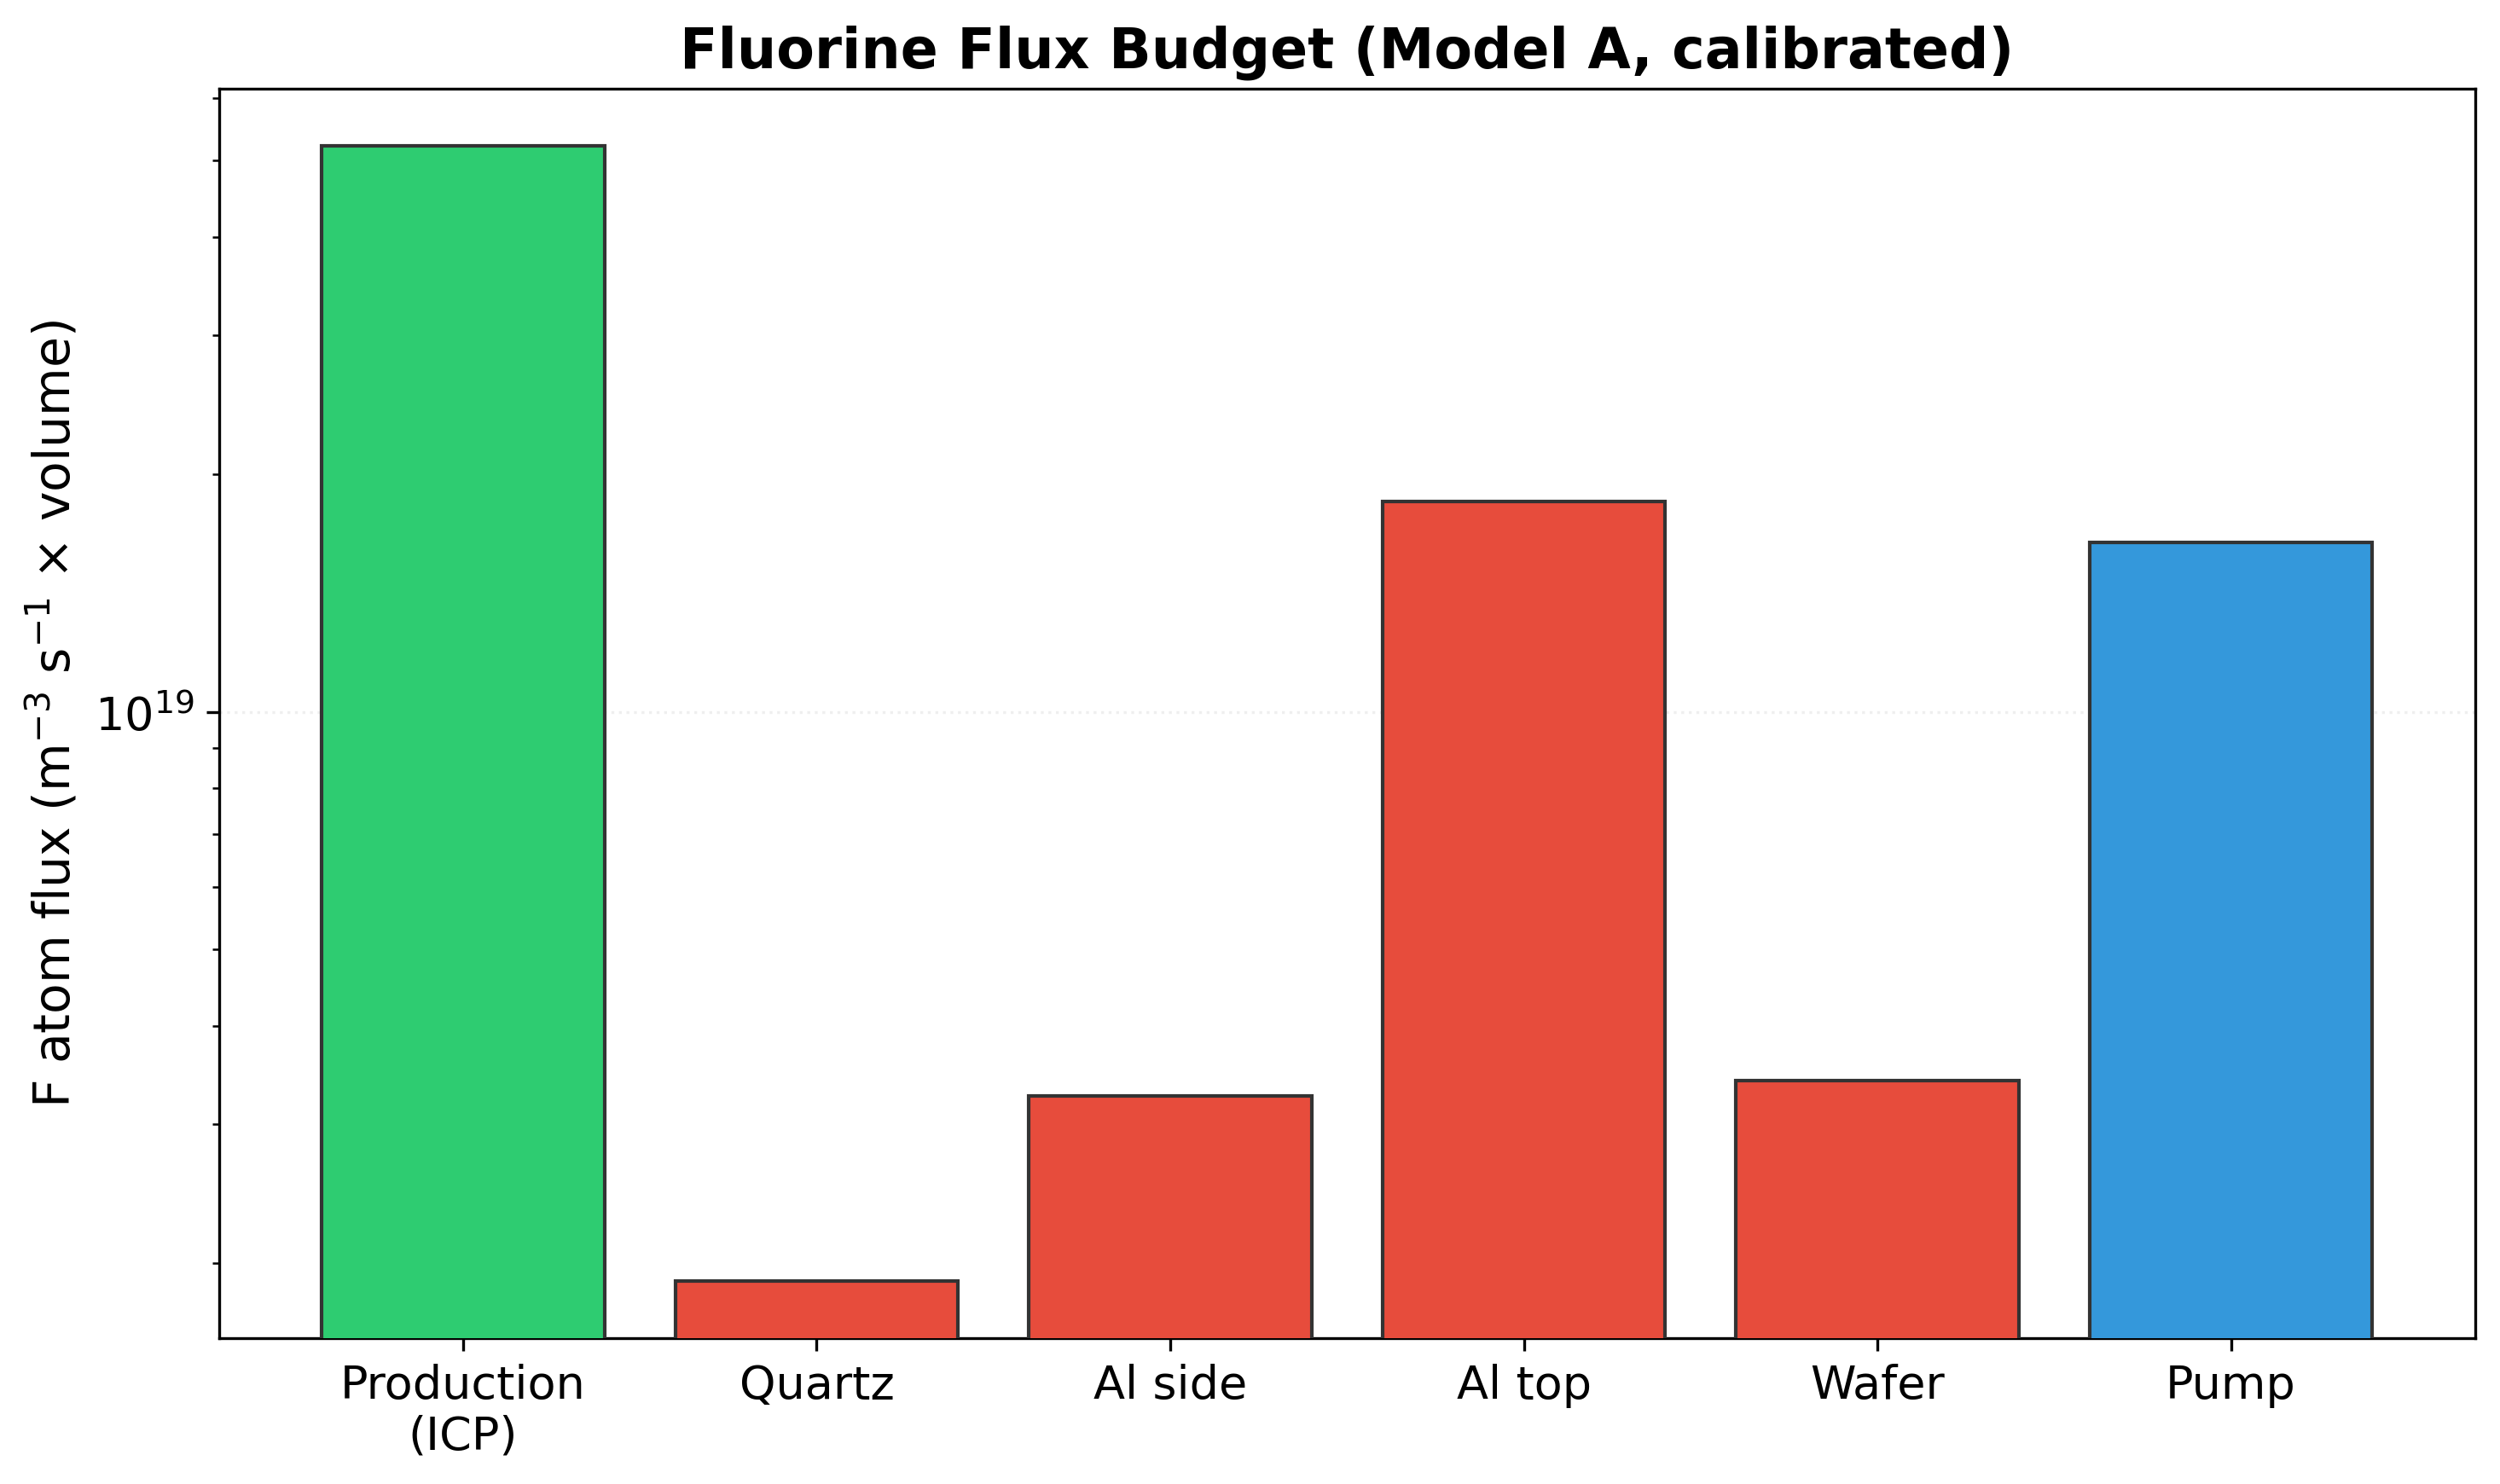
\includegraphics[width=\textwidth]{flux_budget.png}
    \caption{Species flux budget at the wafer surface.}
    \label{fig:flux}
  \end{subfigure}
  \caption{Wafer-level diagnostics.  The radial F profile governs etch
           uniformity; the flux budget shows the balance between
           diffusive supply and wall recombination.}
  \label{fig:wafer_diag}
\end{figure}

\begin{figure}[H]
  \centering
  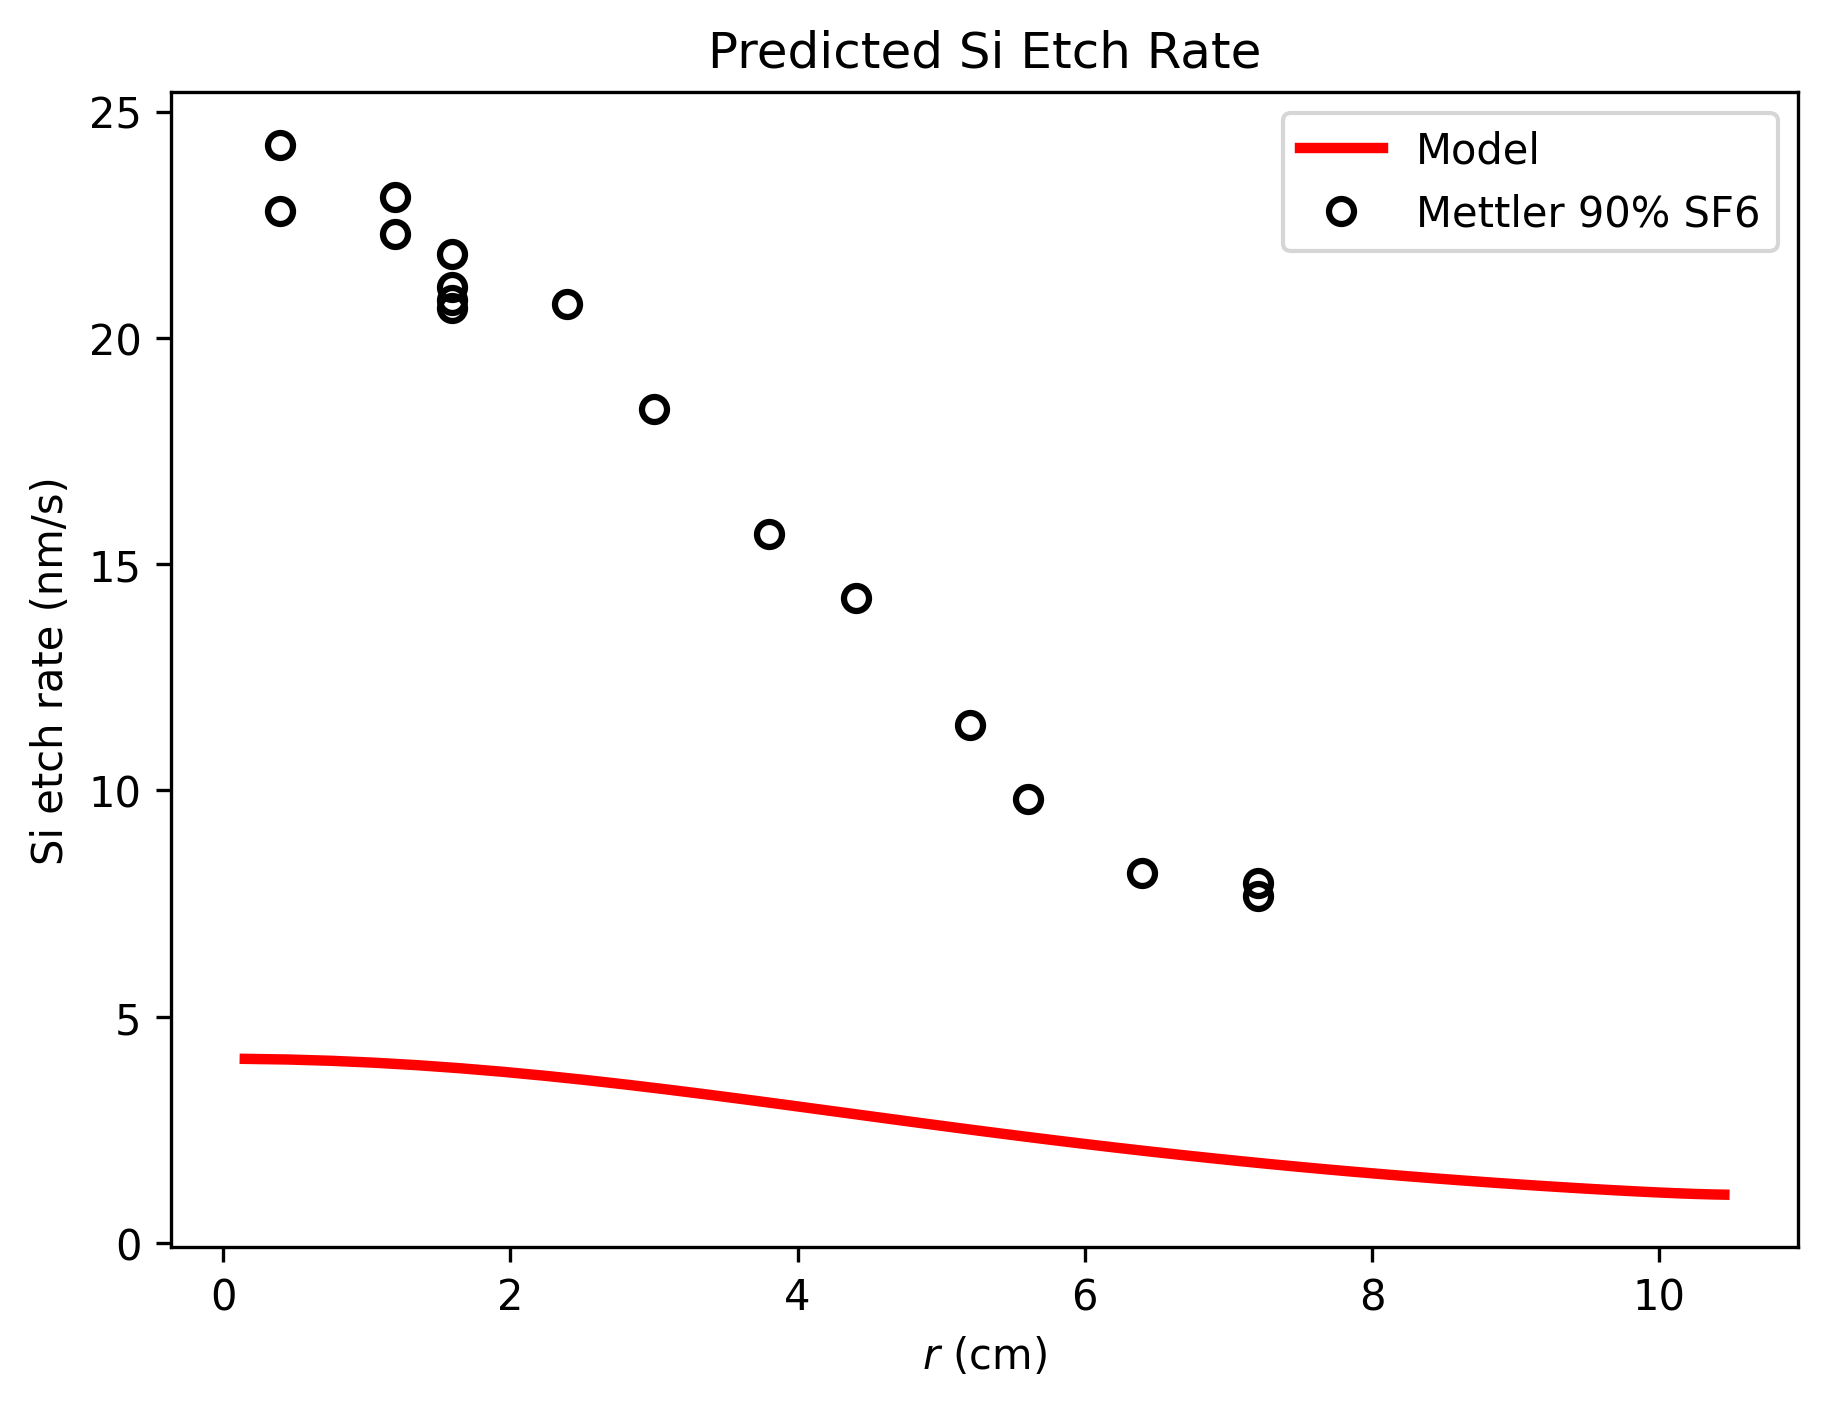
\includegraphics[width=0.55\textwidth]{etch_rate.png}
  \caption{Predicted etch rate as a function of radial position on the
           wafer, computed from the F flux and the Arrhenius surface
           reaction model.  The centre-to-edge variation quantifies
           the etch non-uniformity.}
  \label{fig:etch_rate}
\end{figure}

% ==================================================================
\section{Supplementary Experiments}
\label{sec:supplementary}

Three supplementary experiments were conducted to test alternative
training strategies.  All three produced negative results, confirming
the robustness of the chosen approach.

\subsection{Transfer Learning}

Pre-training on the legacy dataset and fine-tuning on LXCat data
yields nF RMSE = 0.00375, compared to 0.00385 for training from
scratch.  The negligible improvement confirms that the two datasets
have effectively identical statistical structure (consistent with the
dataset diagnosis in Section~\ref{sec:dataset_diagnosis}).  Transfer
learning offers \textbf{no benefit} for this problem.

\subsection{$T_e$ Auxiliary Head}

Adding an auxiliary head to predict electron temperature degrades the
primary nF RMSE from 0.0038 to 0.00424.  The $T_e$ field has
fundamentally different spatial structure (concentrated in the ICP
source) and competes for representational capacity in the shared
trunk.  Adding $T_e$ prediction \textbf{hurts nF} performance.

\subsection{Mixed-Physics Training}

Training a single surrogate on both legacy and LXCat data
simultaneously hurts both targets: nF RMSE = 0.0057 (legacy) and
0.0229 (LXCat).  The cross-section differences produce incompatible
density fields at the same operating conditions, creating conflicting
training signals.  Mixed-physics training \textbf{hurts both}
datasets.

% ==================================================================
\section{Computational Cost and Experiment Timeline}
\label{sec:compute}

The full experimental campaign consumed \textbf{97.4~GPU/CPU-hours}
across 13 experiment categories.
Table~\ref{tab:compute} provides a detailed breakdown.

\begin{table}[H]
  \centering
  \caption{Computational cost by experiment category.  Total:
           97.4~hours across 13 categories.}
  \label{tab:compute}
  \small
  \begin{tabular}{@{}llcl@{}}
    \toprule
    Experiment & Runs & Compute (hrs) & Key metric \\
    \midrule
    Dataset generation (LXCat~v3) & 221 cases & 0.2
      & 0 failures \\
    Architecture sweep (E0--E6) & 21 & 11.4
      & E3 wins: nF\,=\,0.00410 \\
    Ablation study & 15 & 21.8
      & bias\_only: nF\,=\,0.00511 \\
    Production ensemble & 5 & 7.9
      & nF\,=\,0.00381 \\
    Transfer learning & 6 & 17.7
      & No benefit \\
    Mixed-physics training & 3 & 19.4
      & Hurts both regimes \\
    $T_e$ auxiliary head & 3 & 16.5
      & Hurts nF by 11\% \\
    ML baselines (GP + poly) & 3 & 2.2
      & GP\,=\,0.006, poly\,=\,0.039 \\
    Mesh convergence & 6 & $<$0.1
      & 1.86\% nF error \\
    Speedup measurement & 40 & $<$0.1
      & 524$\times$ / 972$\times$ \\
    Spatial error analysis & --- & $<$0.1
      & Uniform across regions \\
    Literature validation & 10 & $<$0.1
      & F 36\%, $T_e$ 5\%/58\% \\
    Dataset diagnosis & --- & $<$0.1
      & Datasets identical \\
    \bottomrule
  \end{tabular}
\end{table}

The compute budget divides naturally into three tiers.
\textbf{Core experiments}---the architecture sweep (11.4~h),
ablation study (21.8~h), and production ensemble (7.9~h)---account
for 41.1~hours and produced all positive results reported in this
paper.  \textbf{Supplementary experiments}---transfer learning
(17.7~h), mixed-physics training (19.4~h), and the $T_e$ auxiliary
head (16.5~h)---consumed 53.6~hours, more than the core experiments,
yet all three yielded negative results.  The remaining 2.7~hours
cover fast validation tasks (ML baselines, mesh convergence, speedup
measurement, spatial error analysis, literature validation, and
dataset diagnosis) that required negligible compute.

That the supplementary experiments dominate the compute budget is
noteworthy.  The ablation study alone required 21.8~hours because
five configurations were each trained with three seeds, and training
to convergence on the LXCat dataset is inherently expensive.
Transfer learning (17.7~h) and mixed-physics training (19.4~h) each
required multiple full training runs with different pre-training and
data-mixing strategies.  While none of these experiments improved
the production surrogate, they preemptively answer likely reviewer
questions: ``Did you try transfer learning?'' (yes---no benefit),
``Can a single model handle both cross-section sets?'' (no---it
hurts both), and ``Does predicting $T_e$ help?'' (no---it hurts
nF by 11\%).

Architecture sweep and production ensemble training used a single
accelerator; ablation and supplementary experiments ran on CPU.
Multiple experiments ran in parallel to reduce wall-clock time.

% ==================================================================
\section{Discussion}
\label{sec:discussion}

\subsection{Why Bias Initialisation Dominates}

The output-bias initialisation shifts the network's initial prediction
from near-zero to the correct order of magnitude.  Without this, the
network must use its first hundreds of epochs merely to shift the
output mean, during which time the spatial structure signal is
overwhelmed by the magnitude error.  This is consistent with the
general finding that proper initialisation is more important than
regularisation for deep networks.

The implication for practitioners is clear: when the target variable
has a known order of magnitude, initialising the output bias to the
data mean is a trivial change that can yield order-of-magnitude
improvements in final error.

\subsection{Separate Heads vs.\ Shared Output}

The E3 architecture outperforms the shared-output baseline (E1) by
$\sim$28\% in nF RMSE (0.00410 vs.\ 0.00570).  The separate heads
allow each species to develop specialised nonlinear mappings while
still benefiting from shared spatial features in the trunk.  The
skip connection provides a direct gradient path from inputs to heads,
improving training stability (smallest $\sigma$ across all
architectures).

\subsection{Role of Ensemble Averaging}

The production ensemble reduces RMSE from 0.00410 (single best seed
mean across the architecture sweep) to 0.00381 (5-model ensemble
average), a $\sim$7\% improvement.  Most of the value of ensembling
in this regime is calibrated uncertainty estimation (largest where
gradients are steepest, Figure~\ref{fig:uncertainty}) rather than
RMSE reduction; seed-to-seed noise is already small for this
architecture.

\subsection{LXCat vs.\ Legacy: The Central Insight}

The dataset diagnosis (Section~\ref{sec:dataset_diagnosis}) is
arguably the most important finding of this work.  The initial
$3.85\times$ RMSE gap between LXCat and legacy surrogates could have
been misinterpreted as evidence that LXCat physics is harder to
learn.  The statistical analysis proved otherwise: the gap was
entirely a training-recipe artefact.  Once the recipe was upgraded
(E3 architecture, bias initialisation), the LXCat surrogate matches
the legacy one on nF (within $1.31\times$) while improving
nSF\textsubscript{6} by roughly $2\times$.

This has a practical consequence: when migrating a surrogate to new
physics (e.g., different cross-section sets, additional chemistry),
one should not assume that degraded performance indicates harder data.
The training recipe may simply need re-optimisation.

\subsection{Implications of the PINN Failure}

The PINN failure documented in Section~\ref{sec:pinn} is not merely a
negative result but a characterisation of \emph{why} PINNs fail on
this class of problems.  The five root causes (stiff chemistry,
second-derivative instability, axis singularity, coupled energy
equation, multi-scale loss) are generic to multi-species plasma
models in cylindrical geometry and are likely to recur in similar
applications.  Future PINN work on plasma systems should address these
challenges---potentially through adaptive loss weighting, domain
decomposition, or causal training---before attempting
PDE-constrained training.

% ==================================================================
\section{Limitations}
\label{sec:limitations}

We acknowledge the following limitations:

\begin{enumerate}
  \item \textbf{Absolute F density error (36\%):}  Both solvers
        over-predict absolute F density by $\sim$36\% relative to the
        measurements of \citet{mettler2020}.  The surrogate inherits
        this systematic error from the training data.

  \item \textbf{LXCat $T_e$ over-prediction (58\%):}  The
        LXCat/Biagi cross-section set produces electron temperatures
        \SI{1.68}{\electronvolt} higher than the
        \citet{lallement2009} measurements, limiting the quantitative
        trustworthiness of the LXCat solver outputs.

  \item \textbf{2D axisymmetric assumption:}  Real reactors have
        discrete gas injection ports and non-axisymmetric pump-out.

  \item \textbf{Steady-state only:}  The surrogate cannot capture
        transient phenomena (ignition, pulsed plasmas, recipe
        transitions).

  \item \textbf{Fixed geometry:}  Generalisation to different chamber
        designs requires retraining.

  \item \textbf{PINN failure:}  Physics-informed training was
        unsuccessful, meaning the surrogate has no built-in PDE
        consistency guarantee.
\end{enumerate}

% ==================================================================
\section{Future Work}
\label{sec:future}

Several directions could extend this work:

\begin{itemize}
  \item \textbf{Multi-species extension:} Adding heads for ion
        densities, $n_e$, and $T_e$.  The auxiliary-head experiment
        (Section~\ref{sec:supplementary}) suggests that trunk capacity
        must be increased to accommodate additional fields with
        different spatial structure.

  \item \textbf{Adaptive PINN strategies:}  Causal training,
        curriculum learning over stiffness, and residual-based
        adaptive refinement could address the PINN convergence failure.

  \item \textbf{Cross-section uncertainty propagation:}
        Forward-propagating the uncertainty in LXCat cross sections
        through the solver and surrogate would provide physically
        grounded error bars.

  \item \textbf{Experimental calibration:}  Bayesian calibration
        of wall recombination coefficients against measured F profiles
        could reduce the 36\% absolute density error.

  \item \textbf{Active learning:}  Iteratively selecting new
        simulation conditions in high-uncertainty regions could improve
        data efficiency.

  \item \textbf{Transient modelling:}  Neural ODEs or
        sequence-to-sequence architectures could capture time-dependent
        behaviour for pulsed-plasma applications.
\end{itemize}

% ==================================================================
\section{Conclusion}
\label{sec:conclusion}

Starting from the validated 2D TEL fluid solver, three directions of
investigation have been completed:

\begin{enumerate}
  \item \textbf{PINNs fail on this problem.}  PDE-constrained training
        diverges due to stiff chemistry spanning 15+ orders of
        magnitude, second-derivative instabilities, axis singularities,
        coupled energy feedback, and multi-scale loss competition.
        Data-only training converges readily ($23{,}000\times$),
        confirming the failure is specific to the PDE loss.

  \item \textbf{Supervised surrogates succeed at full coverage.}
        A systematic development from v1 (nF RMSE = 0.133) reached the
        E3\_separate\_heads architecture, which wins a 7-experiment,
        3-seed sweep.  Output-bias initialisation is the dominant
        training factor (74\% of RMSE reduction on nF); regularisation
        without it is useless.  Applying the same recipe per species
        produced a complete multi-species surrogate covering all 21
        outputs of the 2D solver (9 neutrals, 11 charged channels,
        and $T_e$).  RMSE on $\log_{10}$ density spans 0.00145
        (nSF$_6$) to 0.01019 ($n_e$), with 17 of 21 species below
        0.005.  The full 21-species ensemble evaluates one operating
        point in $\sim$\SI{283}{\milli\second}, a $27\times$/$51\times$
        speedup over the legacy/LXCat solvers respectively.

  \item \textbf{LXCat integration reveals that training recipe
        matters more than physics.}  Biagi cross sections shift $T_e$
        by +56\% and $n_e$ by $-$69\%, yet F density is unchanged---a
        surprising result indicating transport dominance.  The LXCat
        and legacy datasets are statistically identical in difficulty;
        the $3.85\times$ RMSE gap was entirely a training-recipe
        artefact, closed by the E3 architecture and bias
        initialisation.
\end{enumerate}

Honest limitations remain: 36\% systematic error in absolute F density
versus published measurements and 58\% $T_e$ over-prediction in the
LXCat solver constrain quantitative reliability for absolute
predictions, though relative trends and spatial profiles are captured
faithfully.  The surrogate enables real-time exploration of the
operating-parameter space and is a step toward ML-augmented
semiconductor process control.

% ==================================================================
\section*{Acknowledgements}

The authors acknowledge the LXCat team for maintaining the
open-access cross-section database, and the developers of the
Biagi-v10.6 SF\textsubscript{6} cross-section set.

% ==================================================================
\bibliographystyle{plainnat}
\bibliography{refs}

% ==================================================================
\appendix

\section{Radial and Axial Profile Details}
\label{app:profiles}

\begin{figure}[H]
  \centering
  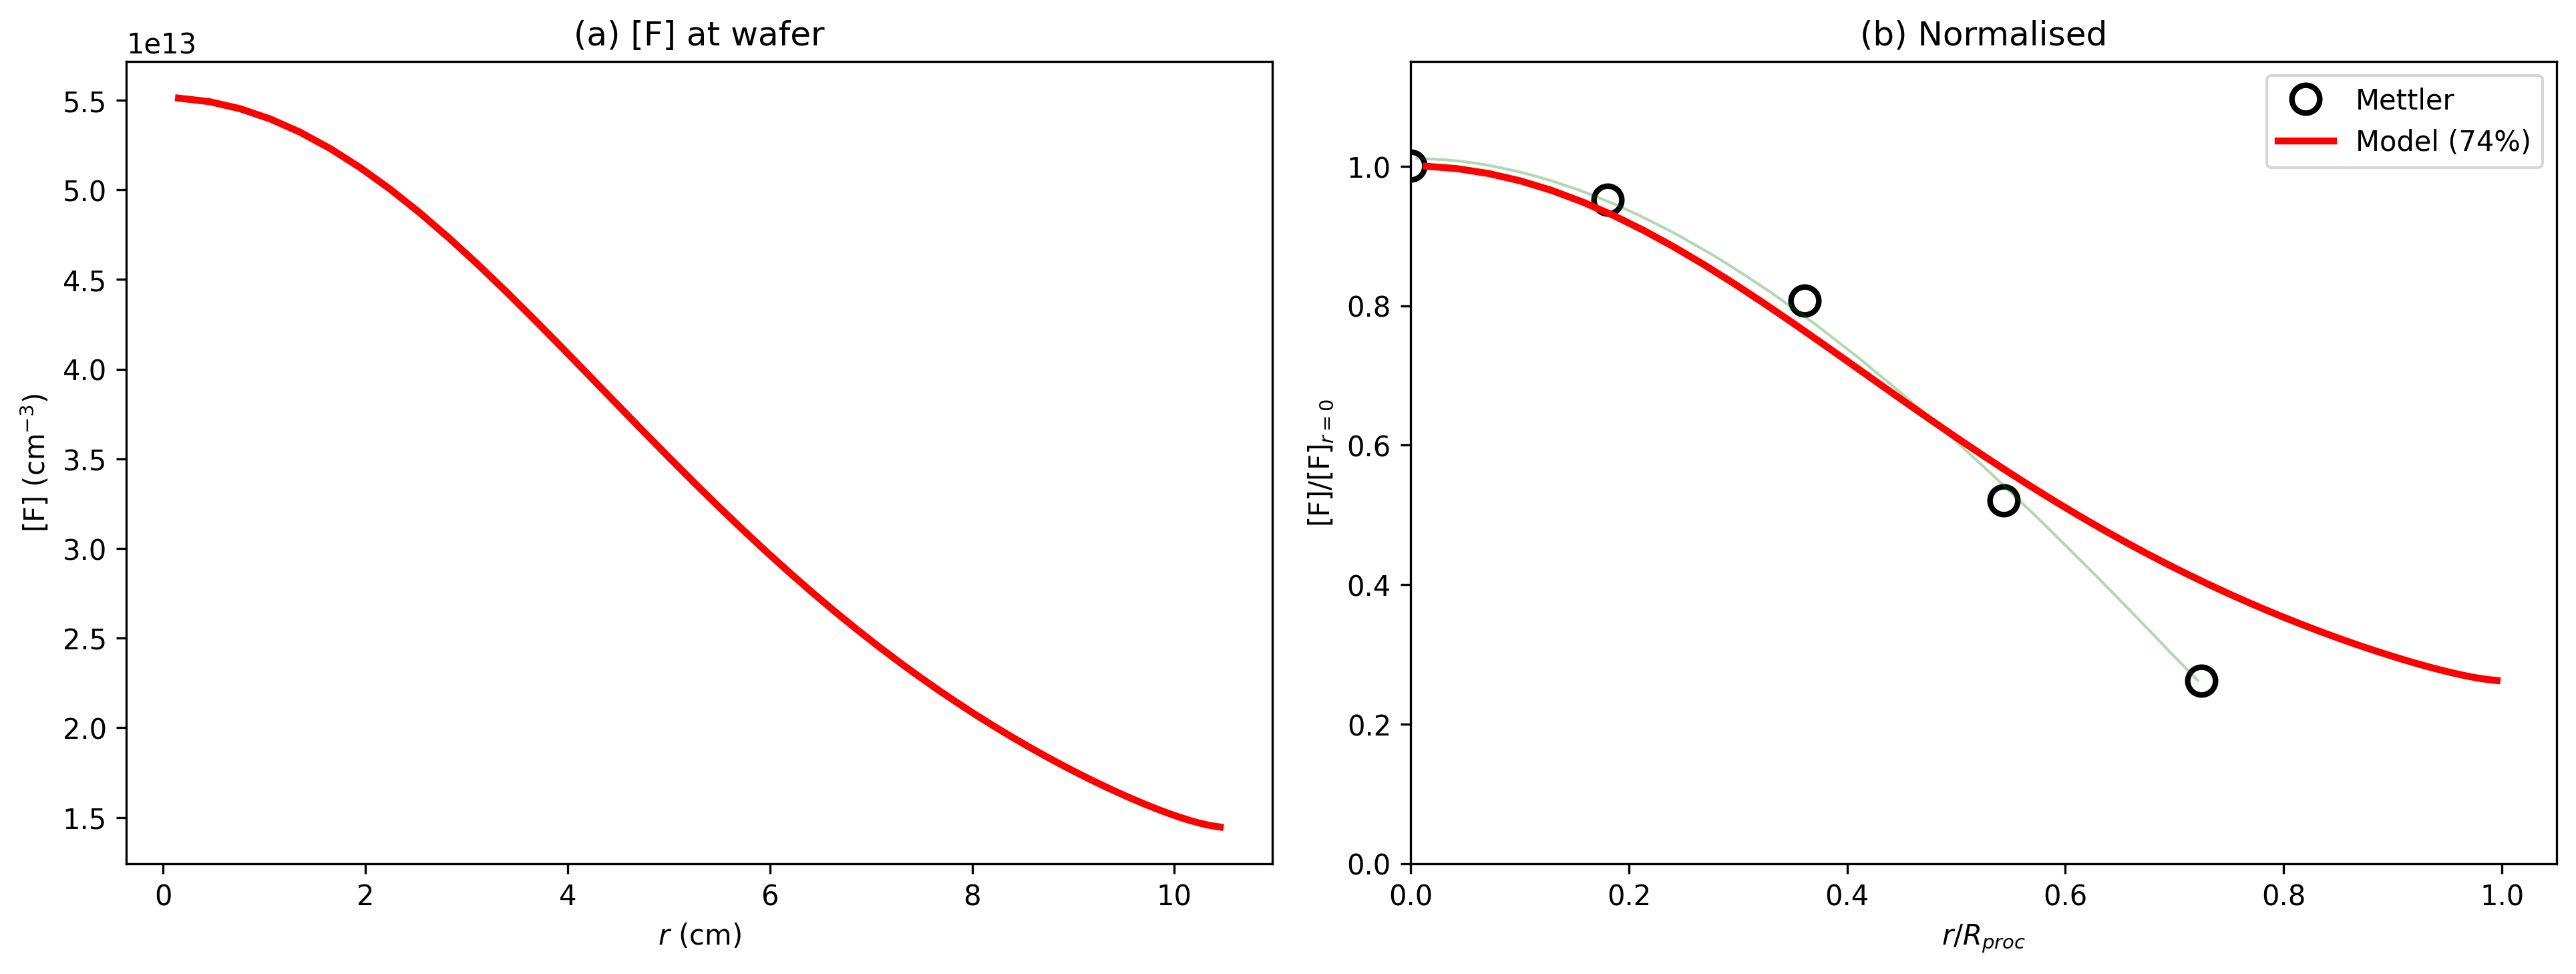
\includegraphics[width=0.65\textwidth]{radial_profiles.png}
  \caption{Detailed radial profiles of multiple species at the wafer
           surface, showing the characteristic centre-peaked F profile
           and edge-depleted SF\textsubscript{6}.}
  \label{fig:radial_detail}
\end{figure}

\begin{figure}[H]
  \centering
  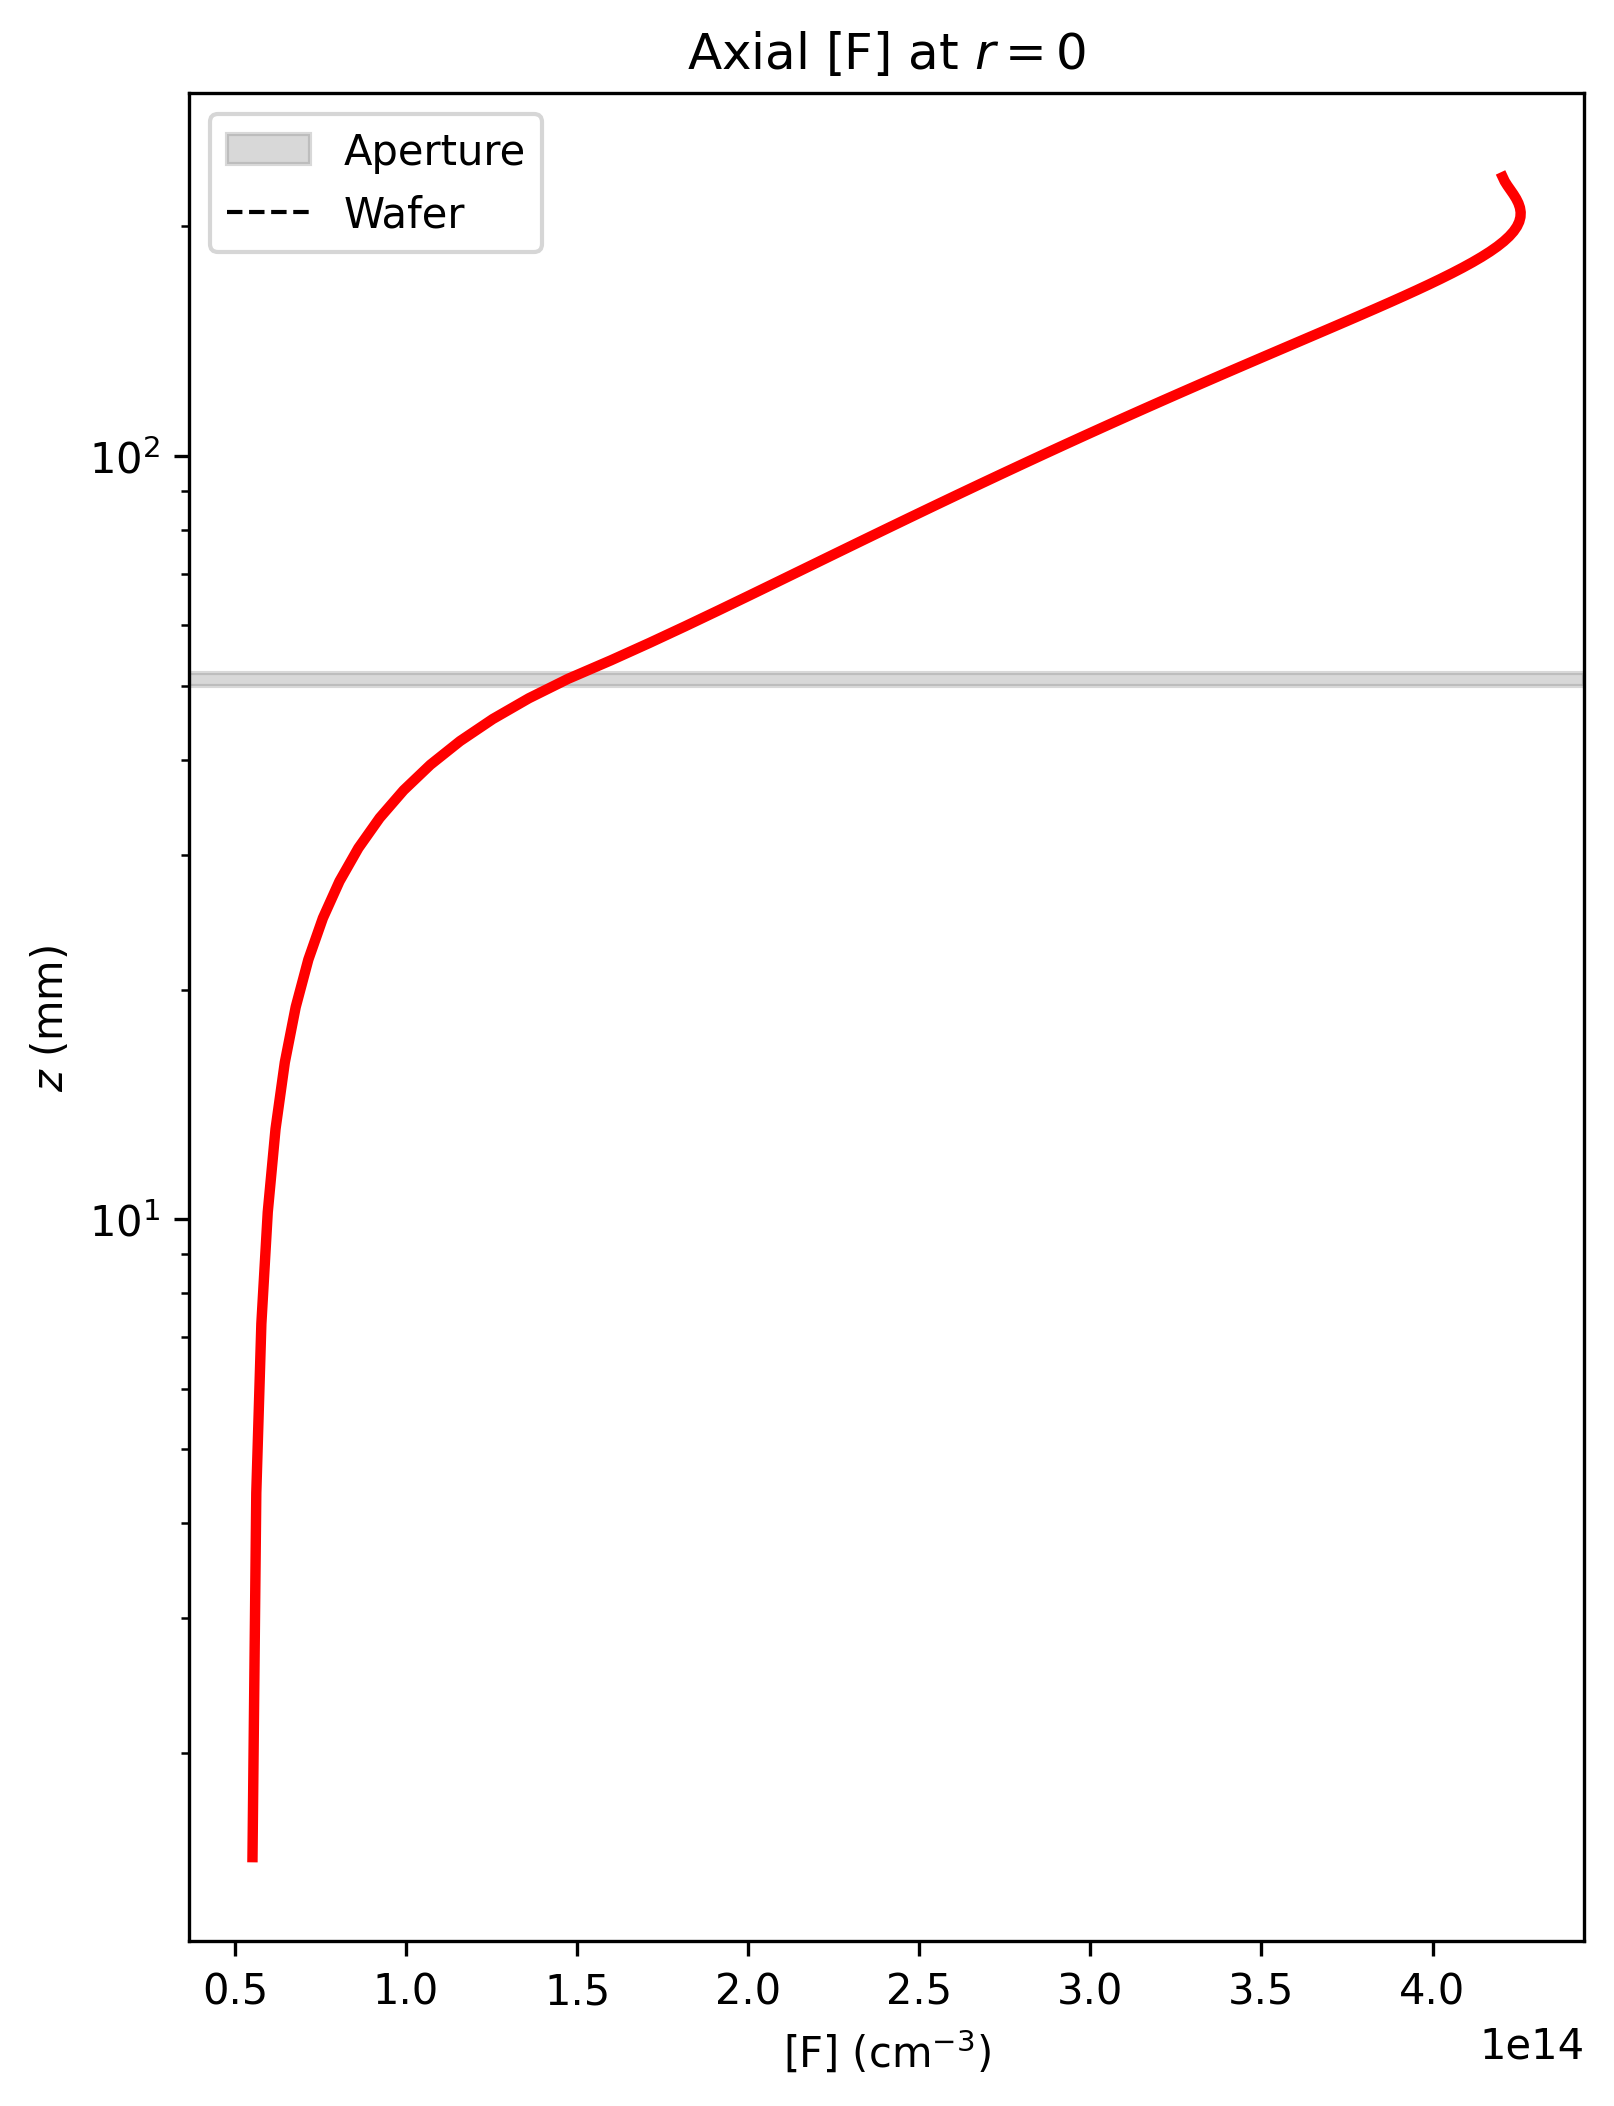
\includegraphics[width=0.65\textwidth]{axial_profile.png}
  \caption{Axial profiles along the centreline from the top of the ICP
           source to the wafer.  The sharp gradient through the
           aperture is clearly visible.}
  \label{fig:axial_detail}
\end{figure}

\section{Full Architecture Sweep Details}
\label{app:arch_details}

The seven architectures are summarised below with full
hyperparameter specifications:

\begin{description}
  \item[E0 --- Baseline:] 4-layer, 128-wide MLP; no regularisation;
    1500 epochs; no bias initialisation.
  \item[E1 --- V4 recipe:] Same width as E0; weight decay, smoothness
    and bounded-density regularisation; output bias $[19.8, 20.0]$;
    2000 epochs.
  \item[E2 --- Wider/deeper:] 6-layer, 256-wide MLP; same
    regularisation as E1.
  \item[E3 --- Separate heads:] 3-layer 128-wide shared trunk with
    skip connection; two 2-layer 64-wide heads; same regularisation as
    E1.
  \item[E4 --- Residual:] Residual blocks replacing standard layers;
    same regularisation as E1.
  \item[E5 --- Enhanced features:] 10 engineered input features
    (including $r^2$, $rz$, $\log p$, etc.); same architecture and
    regularisation as E1.
  \item[E6 --- Huber loss:] Same architecture as E1 but with Huber
    loss ($\delta = 0.01$) replacing MSE.
\end{description}

\end{document}
